\documentclass[cjk]{beamer}
\mode<presentation>{
%  \usetheme{Warsaw}
  \usetheme{CambridgeUS}
  \usecolortheme{beaver}
  %% \setbeamercovered{transparent} 
}
%% \usepackage[T1]{fontenc} % Needed for Type1 Concrete
%% %% \usepackage{concrete} % Loads Concrete + Euler VM
%% %% \usepackage{pxfonts} % Or palatino or mathpazo
%% \usepackage{eulervm} %
%% %% \usepackage{kerkis} % Kerkis roman and sans
%% %% \usepackage{kmath} % Kerkis math
%% \usepackage{fourier}
\usepackage{pgf}
\usepackage{tikz}
\usetikzlibrary{calc}
\usetikzlibrary{arrows,snakes,backgrounds,shapes}
\usetikzlibrary{matrix,fit,positioning,decorations.pathmorphing}
\usepackage{CJK} 
\usepackage{amsmath,amssymb,amsfonts}
\usepackage{mathdots}
\usepackage{subfigure}
\usepackage{caption}
\usepackage{verbatim,color,xcolor}
\usepackage{graphicx}
\usepackage{manfnt}
\usepackage{fancybox}
\usepackage{textcomp}
\usepackage{multirow,multicol}
\usepackage{parcolumns}
\usepackage{framed}
\usepackage{threeparttable}
\usepackage{extarrows}
\usepackage{listings}
\lstset{
  keywordstyle=\color{blue!70},
  frame=lines,
  basicstyle=\ttfamily\small,
  commentstyle=\small\color{red},
  rulesepcolor=\color{red!20!green!20!blue!20},
  tabsize=4,
  numbersep=5pt,
  backgroundcolor=\color[rgb]{0.95,1.0,1.0},
  showspaces=false,
  showtabs=false,
  extendedchars=false,
  escapeinside=``
}
%% \usepackage[utf8]{inputenc}
%% \usepackage[upright]{fourier}   %

% ######### DEFINE COLOR ###############
\definecolor{blue}{rgb}{0.0,0.0,1.0}
\definecolor{red}{rgb}{1.0,0.0,0.0}
%\definecolor{purple}{rgb}{1.0,0.0,0.0}
\definecolor{electricpurple}{rgb}{0.75, 0.0, 1.0}

%%%% \renewcommand *****
\renewcommand{\lstlistingname}{}
\newcommand{\tf}{\ttfamily}
\newcommand{\ttt}{\texttt}
\newcommand{\blue}{\textcolor{blue}}
\newcommand{\red}{\textcolor{red}}
\newcommand{\purple}{\textcolor{purple}}
\newcommand{\ft}{\frametitle}
\newcommand{\bs}{\boldsymbol}
\newcommand{\disp}{\displaystyle}
\newcommand{\ds}{\displaystyle}
\newcommand{\vd}{\vdots}
\newcommand{\cd}{\cdots}
\newcommand{\dd}{\ddots}
\newcommand{\id}{\iddots}
\newcommand{\XX}{\mathbf{X}}
\newcommand{\PP}{\mathbf{P}}
\newcommand{\QQ}{\mathbf{Q}}
\newcommand{\xx}{\mathbf{x}}
\newcommand{\yy}{\mathbf{y}}
\newcommand{\bb}{\mathbf{b}}
\newcommand{\aaa}{\mathbf{a}}
\newcommand{\A}{\mathbf{A}}
\newcommand{\B}{\mathbf{B}}
\newcommand{\C}{\mathbf{C}}
\newcommand{\D}{\mathbf{D}}
\newcommand{\E}{\mathbf{E}}
\newcommand{\U}{\mathbf{U}}
\newcommand{\X}{\mathbf{X}}
\newcommand{\Y}{\mathbf{Y}}
\newcommand{\Z}{\mathbf{Z}}
\newcommand{\T}{\mathbf{T}}
\newcommand{\zero}{\mathbf{0}}
\newcommand{\II}{\mathbf{I}}
\newcommand{\ii}{\mathbf{i}}
\newcommand{\jj}{\mathbf{j}}
\newcommand{\kk}{\mathbf{k}}
\newcommand{\uu}{\mathbf{u}}
\newcommand{\vv}{\mathbf{v}}
\newcommand{\ee}{\mathbf{e}}
\newcommand{\Lambdabd}{\mathbf{\Lambda}}
\newcommand{\alphabd}{\boldsymbol{\alpha}}
\newcommand{\betabd}{\boldsymbol{\beta}}
\newcommand{\gammabd}{\boldsymbol{\gamma}}
\newcommand{\xibd}{\boldsymbol{\xi}}
\newcommand{\epsilonbd}{\boldsymbol{\epsilon}}
\newcommand{\etabd}{\boldsymbol{\eta}}
\newcommand{\rr}{\mathrm{r}}
\newcommand{\RR}{\mathrm{R}}
\newcommand{\RRR}{\mathbb{R}}
\newcommand{\CCC}{\mathbb{C}}




\begin{document}
\begin{CJK}{UTF8}{gkai} 
  \CJKtilde
  \renewcommand{\proofname}{\vspace{0.2cm}\textbf{\blue{证明: \ }}}
  \newcommand{\jiename}{\vspace{0.2cm}\textbf{\blue{解: \ }}}
  
  \renewcommand{\figurename}{图}  
  \title{线性代数}
\subtitle{总复习}
\institute[]{
  
\includegraphics[width=0.5in]{wuda_log.pdf} \\
  数学与统计学院 \\
  Email: ~~ xpzhang.math@whu.edu.cn    \\
  Homepage: ~~http://staff.whu.edu.cn/show.jsp?n=Zhang\%20Xiaoping
}

\author{张晓平}
\date{}
\subject{线性代数}
% 如果你想插入学校的徽章, 其文件名为 "university-logo-filename.xxx", 
% 其中 xxx 是 pdflatex 能接受的格式, 则可用以下命令插入
%% \pgfdeclareimage[height=0.5cm]{wuda}{wudalogo.pdf}
%% \logo{\pgfuseimage{wuda}}
%% \pgfdeclareimage[width=1.0cm]{university-logo}{university-logo-filename.jpg}
%% \logo{\pgfuseimage{university-logo}}

% 如果你想要在每一小节之前都显示一下目录, 则可把一下小段的注解号 "%" 删去
%% \AtBeginSubsection[]
%% {
%%  \begin{frame}<beamer>
%%    \frametitle{概要}
%%    \tableofcontents[currentsection,currentsubsection]
%%  \end{frame}
%% }

%除掉以下命令的注解 "%" 后, 许多环境都会自动逐段显示
% \beamerdefaultoverlayspecification{<+->}

%% 的演示文稿仅供参考, 不过可以提供一些忠告:
% - 除总结外, 最好不超过 3 节;
% - 每节至多分成 3 小节;
% - 每屏约 30 秒至 2 分钟, 因此总共 15 至 30 屏为佳.
% - 一般说来, 会议听众对你所报告的东西知之甚少, 因此尽量简单!
% - 在 20 分钟报告里只要讲清主要思想即可, 不要深入细节, 宁可牺牲一点严格性;
% - 如果你略去了证明或实现的关键细节, 只要声明一下即可, 没有人会感到不高兴.

  
  
  \begin{frame}
    \titlepage
  \end{frame}

  \begin{frame}
    \frametitle{目录}
    \tableofcontents[currentsection,sectionstyle=show]
  \end{frame}

  \AtBeginSection[]{
    \begin{frame}[allowframebreaks]
      \tableofcontents[currentsection]%,hideallsubsections]
    \end{frame}
  }
  \AtBeginSubsection[]{
    \begin{frame}[shrink]
      \tableofcontents[sectionstyle=show/shaded,subsectionstyle=show/shaded/hide]
    \end{frame}
  }

\documentclass[10pt,a4paper%,twoside,openright,titlepage,fleqn,%
% headinclude,footinclude,BCOR5mm,%
% numbers=noenddot,cleardoublepage=empty,%
tablecaptionabove]{article}

\usepackage{geometry}
\geometry{left=2.5cm,right=2.5cm,top=2.5cm,bottom=2.5cm}
%\usepackage{subfigure}
\usepackage{amsmath,amssymb,amsthm}

%% -----------------设置数学公式字体-------------------------
%% Font style 1
%% \newcommand\ibinom[2]{\genfrac\lbrace\rbrace{0pt}{}{#1}{#2}}
%% \usepackage{bm}

%% Font style 2
%% \newcommand\ibinom[2]{\genfrac\lbrace\rbrace{0pt}{}{#1}{#2}} 
%% \usepackage[boldsans]{ccfonts} 
%% \usepackage{bm} 

%% Font style 3
\newcommand\ibinom[2]{\genfrac\lbrace\rbrace{0pt}{}{#1}{#2}}
\usepackage[euler-digits]{eulervm}
\usepackage{bm}

%% Font style 4
%% \usepackage{fourier}
%% \newcommand\ibinom[2]{\genfrac\lbrace\rbrace{0pt}{}{#1}{#2}}
%% \usepackage{bm}

%% Font style 5
%% \newcommand\ibinom[2]{\genfrac\lbrace\rbrace{0pt}{}{#1}{#2}}
%% \usepackage{mathptmx}
%% \usepackage{bm} 


%% %% Font style 6
%% \newcommand\ibinom[2]{\genfrac\lbrace\rbrace{0pt}{}{#1}{#2}}
%% \usepackage{txfonts}
%% \usepackage{bm}
%% -----------------------------------------------------------

 


\usepackage{extarrows}
\usepackage{verbatim,color,xcolor}
\usepackage{pgf}
\usepackage{tikz}
\usetikzlibrary{calc}
\usetikzlibrary{arrows,snakes,backgrounds,shapes,patterns}
\usetikzlibrary{matrix,fit,positioning,decorations.pathmorphing}
%% \usepackage{classicthesis}
\usepackage{CJK}
\usepackage{mathdots}

\usepackage{listings}
\lstset{
  keywordstyle=\color{blue!70},
  frame=single,
  basicstyle=\ttfamily\small,
  commentstyle=\small\color{red},
  breakindent=0pt,
  rulesepcolor=\color{red!20!green!20!blue!20},
  rulecolor=\color{black},
  tabsize=4,
  numbersep=5pt,
  breaklines=true,
  %% backgroundcolor=\color{red!10},
  showspaces=false,
  showtabs=false,
  extendedchars=false,
  escapeinside=``,
  frame=no,
}
\renewcommand{\proofname}{\textbf{证明}}
\renewcommand{\figurename}{\textbf{图}}
\newcommand{\blue}{\textcolor{blue}}
\newcommand{\red}{\textcolor{red}}
\newcommand{\purple}{\textcolor{purple}}
\newcommand{\ds}{\displaystyle}
\newcommand{\cd}{\cdots}
\newcommand{\dd}{\ddots}
\newcommand{\vd}{\vdots}
\newcommand{\id}{\iddots}

\newcommand{\R}{\mathbb R}
\def\nn{{\boldsymbol{n}}}
\def\xx{{\boldsymbol{x}}}
\def\F{{\boldsymbol{F}}}
\def\tf{\ttfamily}


\begin{document}

\begin{CJK}{UTF8}{gkai}
  \renewcommand{\proofname}{\textbf{证明}}
  \renewcommand{\figurename}{\textbf{图}}


  \newtheorem{li}{例}
  \newtheorem{jielun}{结论}
  \newtheorem{dingli}{定理}
  \newtheorem{mingti}{{命题}} 
  \newtheorem{yinli}{{引理}} 
  \newtheorem{tuilun}{{推论}}
  \newtheorem{dingyi}{{定义}} 
  \newtheorem{example}{{例}}
  \newtheorem*{example*}{{例}}
  \newtheorem*{jie}{{解}}
  \newtheorem*{zhengming}{{证明}}
  \newtheorem{zhu}{{注}}
  \newtheorem*{zhu*}{{注}}
  \newtheorem{xingzhi}{{性质}}
  \newtheorem{wenti}{{问题}}
  \newtheorem{rem}{{Remark}}
  \newtheorem{lem}{{Lemma}}
  \pagenumbering{roman}
  \pagestyle{plain}

  \pagenumbering{arabic}

  \title{第一讲、行列式}
  % \author{张晓平}
  % \date{}                                           % Activate to display a given date or no date
  \maketitle

  \section{行列式的定义}
  \subsection{二阶行列式}
  %%%%% 
  \begin{li}
    用消元法求解
    $$
    \left \lbrace
      \begin{array}{l}
        a_{11} x_1 + a_{12} x_2 = b_1, \\[0.2cm]
        a_{21} x_1 + a_{22} x_2 = b_2.
      \end{array}
    \right.
    $$
  \end{li}  
  消去$x_2$得
  $$
  (a_{11}a_{22}-a_{12}a_{21})x_1 = b_1 a_{22} - b_2 a_{12},
  $$
  消去$x_1$得
  $$
  (a_{11}a_{22}-a_{12}a_{21})x_2 = b_2 a_{11} - b_1 a_{11}.
  $$
  若$\boxed{\red{a_{11}a_{22}-a_{12}a_{21}\ne0}}$,则
  $$
  x_1 = \frac{b_1 a_{22} - b_2 a_{12}}{a_{11}a_{22}-a_{12}a_{21}}, \ \
  x_2 = \frac{b_2 a_{11} - b_1 a_{11}}{a_{11}a_{22}-a_{12}a_{21}}.
  $$

  %%%% 
  \begin{dingyi}[二阶行列式]
    由$2^2=4$个数,按下列形式排成2行2列的方形
    $$
    \left|
      \begin{array}{cc}
        a_{11} & a_{12} \\[0.2cm]
        a_{21} & a_{22} 
      \end{array}
    \right|,
    $$
    其被定义成一个数
    $$
    \left|
      \begin{array}{cc}
        a_{11} & a_{12} \\[0.2cm]
        a_{21} & a_{22} 
      \end{array}
    \right| = a_{11}a_{22} - a_{12}a_{21} \equiv D,
    $$
    该数称为由这四个数构成的二阶行列式。
  \end{dingyi}
  %%%% 
  $\red{a_{ij}}$表示行列式的元素。
  $i$为行标,表明该元素位于第$i$行;
  $j$为列标,表明该元素位于第$j$列。
  \begin{figure}[htbp]
    \centering      
    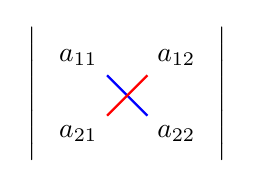
\begin{tikzpicture}
      \matrix (A) [matrix of nodes,ampersand replacement=\&,row sep=15pt,column sep=15pt,left delimiter=|,
      right delimiter=|] {
        $a_{11}$ \& $a_{12}$  \\
        $a_{21}$ \& $a_{22}$  \\
      };
      \draw[blue, thick] (A-1-1.south east) -- (A-2-2.north west);
      \draw[red,  thick] (A-1-2.south west) -- (A-2-1.north east);
    \end{tikzpicture}
    \caption{对角线法则}
  \end{figure}

  %%%%%% 
  
  类似地,
  $$
  \begin{array}{l}
    b_1 a_{22} - b_2 a_{12} = \left|
    \begin{array}{cc}
      b_1 & a_{12} \\
      b_2 & a_{22} 
    \end{array}
            \right|  \equiv D_1\\[0.4cm]
    b_2 a_{11} - b_1 a_{21} = \left|
    \begin{array}{cc}
      a_{11} & b_1 \\
      a_{21} & b_2
    \end{array}
               \right|  \equiv D_2\\
  \end{array}
  $$      
  则上述方程组的解可表示为
  $$
  x_1 = \frac{D_1}{D},\ \
  x_2 = \frac{D_2}{D}.
  $$

  \begin{li}
    求解二元线性方程组
    $$
    \left\{
      \begin{array}{l}
        3x_1 - 2x_2 = 12, \\[0.2cm]
        2x_1 + x_2  = 1.
      \end{array}
    \right.
    $$
  \end{li}
  解:因为
  $$
  \begin{array}{l}
    D = \left|
    \begin{array}{cc}
      3 & -2 \\
      2 & 1 
    \end{array}
          \right| = 7 \ne 0,\\[0.4cm]
    D_1 = \left|
    \begin{array}{cc}
      12 & -2 \\
      1 & 1 
    \end{array}
          \right| = 14 , \\[0.4cm]
    D_2 = \left|
    \begin{array}{cc}
      3 & 12 \\
      2 & 1 
    \end{array}
          \right| = -21,
  \end{array}
  $$
  因此,
  $$
  x_1=\frac{D_1}{D}=2, \ \ x_2 = \frac{D_2}{D} = -3.
  $$

  \subsection{三阶行列式}
  \begin{dingyi}[三阶行列式]
    由$3^2=9$个数组成的3行3列的三阶行列式,则按如下形式定义一个数
    $$
    \begin{aligned}
      D_3 &= 
      \left|
        \begin{array}{ccc}
          a_{11} & a_{12} & a_{13} \\[0.2cm]
          a_{21} & a_{22} & a_{23} \\[0.2cm]
          a_{31} & a_{32} & a_{33} 
        \end{array}
      \right|
      \\
      &=  a_{11}a_{22}a_{33} + a_{12}a_{23}a_{31} + a_{13}a_{21}a_{32}
      - a_{13}a_{22}a_{31} - a_{11}a_{23}a_{32} - a_{12}a_{21}a_{33}
    \end{aligned}
    $$
  \end{dingyi}

  \begin{figure}[htbp]
    \centering
    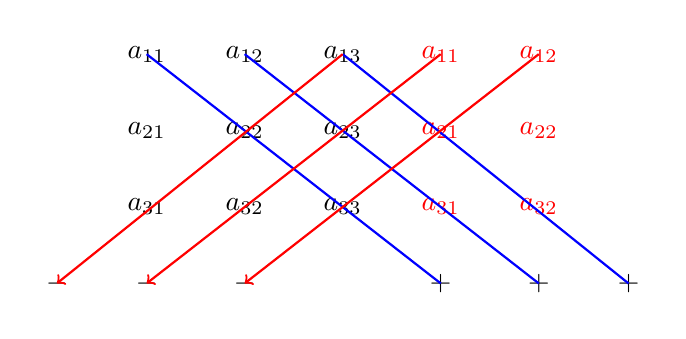
\begin{tikzpicture}               
      \matrix(A) [matrix of math nodes,nodes in empty cells,ampersand replacement=\&,row sep=15pt,column sep=15pt] {
        \&  a_{11} \& a_{12} \& a_{13}  \& \red{a_{11}} \& \red{a_{12}} \&\\
        \&  a_{21} \& a_{22} \& a_{23}  \& \red{a_{21}} \& \red{a_{22}} \&\\
        \&  a_{31} \& a_{32} \& a_{33}  \& \red{a_{31}} \& \red{a_{32}} \&\\
        -   \&    -        \&   -        \&               \&   +         \&   +        \& +\\
      };
      \draw[blue,thick] (A-1-2.center) -- (A-4-5.center);
      \draw[blue,thick] (A-1-3.center)  -- (A-4-6.center);
      \draw[blue,thick] (A-1-4.center) -- (A-4-7.center); 
      \draw[red,thick,->] (A-1-6.center) -- (A-4-3.center);
      \draw[red,thick,->] (A-1-5.center) -- (A-4-2.center);
      \draw[red,thick,->] (A-1-4.center) -- (A-4-1.center); 
    \end{tikzpicture}
    \caption{沙路法}
  \end{figure}

  \begin{li}
    计算
    $$
    D_3 = 
    \left |
      \begin{array}{rrr}
        1  & 2 & -4 \\ 
        -2 & 2 & 1  \\
        -3 & 4 & -2
      \end{array}
    \right|
    $$
  \end{li}
  \begin{jie}
    由沙路法可知,
    $$
    \begin{array}{ll}
      D_3 &=   1\times   2  \times (-2) +   2  \times 1 \times (-3) + (-2) \times 4 \times (-4)\\[0.2cm]
          & - 2\times (-2) \times (-2) - (-4) \times 2 \times (-3) +   1  \times 1 \times   4\\[0.2cm]
          & = -14.
    \end{array}
    $$
  \end{jie}

  \begin{li}
    求方程
    $$
    \left |
      \begin{array}{ccc}
        1  & 1 & 1 \\
        2  & 3 & x  \\
        4  & 9 & x^2
      \end{array}
    \right| = 0
    $$        
  \end{li}
  \begin{jie}
    行列式
    $$ 
    D = 3x^2 + 18 + 4x - 2x^2 - 12 - 9x 
    = x^2 - 5x + 6
    $$
    由此可知$x=2$或$3$。
  \end{jie}


  如果三元一次方程组
  $$
  \begin{array}{c}  
    a_{11}x_1 + a_{12}x_2 + a_{13}x_3 = b_1, \\
    a_{21}x_1 + a_{22}x_2 + a_{23}x_3 = b_2, \\
    a_{31}x_1 + a_{32}x_2 + a_{33}x_3 = b_3,
  \end{array}
  $$
  的系数行列式
  $$
  D = \left|
    \begin{array}{ccc}
      a_{11} & a_{12} & a_{13}\\
      a_{21} & a_{22} & a_{23}\\
      a_{31} & a_{32} & a_{33}
    \end{array}
  \right| \ne 0
  $$
  则用消元法求解可得
  $$
  x_1 = \frac{D_1}{D}, \quad
  x_2 = \frac{D_2}{D}, \quad
  x_3 = \frac{D_3}{D}, \quad
  $$
  其中
  $$
  D_1 = \left|
    \begin{array}{ccc}
      b_1 & a_{12} & a_{13}\\
      b_2 & a_{22} & a_{23}\\
      b_3 & a_{32} & a_{33}
    \end{array}
  \right|, \
  D_2 = \left|
    \begin{array}{ccc}
      a_{11} & b_1 & a_{13}\\
      a_{21} & b_2 & a_{23}\\
      a_{31} & b_3 & a_{33}
    \end{array}
  \right|, \
  D_3= \left|
    \begin{array}{ccc}
      a_{11} & a_{12} & b_1 \\
      a_{21} & a_{22} & b_2 \\
      a_{31} & a_{32} & b_3 
    \end{array}
  \right|.
  $$

  从二、三阶行列式的展开式中可发现:
  $$
  \begin{array}{l}
    D  =  \left|
    \begin{array}{ccc}
      a_{11} & a_{12} & a_{13}\\
      a_{21} & a_{22} & a_{23}\\
      a_{31} & a_{32} & a_{33}
    \end{array}
                        \right| \\[0.6cm]
    = 
    a_{11}a_{22}a_{33}+a_{12}a_{23}a_{31}+a_{13}a_{21}a_{32}
    -a_{13}a_{22}a_{31}-a_{12}a_{21}a_{33}-a_{11}a_{23}a_{32} \\[0.3cm] 
    = 
    a_{11}(a_{22}a_{33}-a_{23}a_{32})-
    a_{12}(a_{21}a_{33}-a_{23}a_{31})+
    a_{13}(a_{21}a_{32}-a_{22}a_{31}) \\[0.3cm] 
    = 
    a_{11} \underbrace{\left| \begin{array}{ccc} a_{22} & a_{33} \\ a_{23} & a_{32} \end{array} \right|}_{M_{11}} -
                                                                             a_{12} \underbrace{\left| \begin{array}{ccc} a_{21} & a_{23} \\ a_{31} & a_{33} \end{array} \right|}_{M_{12}} +
                                                                                                                                                      a_{13} \underbrace{\left| \begin{array}{ccc} a_{21} & a_{22} \\ a_{31} & a_{32} \end{array} \right|}_{M_{13}}
  \end{array}
  $$
  这里,$M_{11},M_{12},M_{13}$分别称为$a_{11},a_{12},a_{13}$的\red{余子式},并称
  $$
  A_{11} = (-1)^{1+1} M_{11}, \quad
  A_{12} = (-1)^{1+2} M_{12}, \quad
  A_{13} = (-1)^{1+3} M_{13}
  $$
  分别称为$a_{11},a_{12},a_{13}$的\red{代数余子式}。 这样,$D$可表示为
  $$
  D= a_{11}A_{11} + a_{11}A_{13} + a_{13}A_{13}.
  $$

  同样地,
  $$
  D = \left| \begin{array}{ccc} a_{11} & a_{12} \\ a_{21} & a_{22} \end{array} \right|
  = a_{11} A_{11} + a_{12} A_{12},
  $$
  其中
  $$
  A_{11} = (-1)^{1+1}|a_{22}| =  a_{22},\quad
  A_{11} = (-1)^{1+2}|a_{21}| = -a_{21}.
  $$
  注意这里的$|a_{22}|,~|a_{21}|$是一阶行列式,而不是绝对值。
  我们把一阶行列式$|a|$定义为$a$。


  \subsection{$n$阶行列式的定义}
  \begin{dingyi}[$n$阶行列式]
    由$n^2$个数$a_{ij}(i,j=1,2,\cdots,n)$组成的$n$阶行列式
    \begin{equation}\label{Dn}
      D = \left|
        \begin{array}{cccc}
          a_{11}  &  a_{12} & \cdots & a_{1n} \\
          a_{21}  &  a_{22} & \cdots & a_{2n} \\
          \vdots & \vdots & \ddots & \vdots\\  
          a_{n1}  &  a_{n2} & \cdots & a_{nn} 
        \end{array}
      \right|
    \end{equation}
    是一个数。
    \begin{itemize}
    \item 当$n=1$时,定义$D=|a_{11}|=a_{11}$; 
    \item 当$n\ge2$时,定义
      \begin{equation}
        D = a_{11} A_{11} + a_{12} A_{12} + \cdots + a_{1n} A_{1n},
      \end{equation}
      其中
      $$A_{1j} = (-1)^{1+j} M_{1j}$$
      而$M_{1j}$是$D$中划去第$1$行第$j$列后,按原顺序排成的$n-1$阶行列式,即
      $$
      M_{1j} =   \left|
        \begin{array}{cccccc}
          a_{21}  & \cdots&  a_{2,j-1}  &  a_{2,j+1}  & \cdots & a_{2n} \\
          a_{31}  & \cdots&  a_{3,j-1}  &  a_{3,j+1}  & \cdots & a_{3n} \\
          \vdots &       &  \vdots &  \vdots &  & \vdots\\  
          a_{n1}  & \cdots&  a_{n,j-1}  &  a_{n,j+1}  & \cdots & a_{nn} 
        \end{array}
      \right| \quad (j = 1,2,\cdots, n),
      $$
      并称$M_{1j}$为$a_{1j}$的余子式,$A_{1j}$为$a_{1j}$的代数余子式.
    \end{itemize}
  \end{dingyi}

  \begin{zhu}
    需注意以下两点:
    \begin{enumerate}
    \item[1]
      在$D$中,$a_{11},a_{22},\cdots,a_{nn}$所在的对角线称为行列式的\red{主对角线},$a_{11},a_{22},\cdots,a_{nn}$称为\red{主对角元}。
    \item[2]
      行列式$D$是由$n^2$个元素构成的$n$次齐次多项式:
      \begin{itemize}
      \item 二阶行列式的展开式有$2!$项;
      \item 三阶行列式的展开式有$3!$项;
      \item $n$阶行列式的展开式有$n!$项,其中每一项都是不同行不同列的$n$个元素的乘积,带正号的项与带负号的项各占一半。
      \end{itemize}      
    \end{enumerate}    
  \end{zhu}
  由行列式的定义可知,一个$n$阶行列式可以展开成$n$个$n$阶行列式之和,即
  $$
  \begin{aligned}
    \left|
      \begin{array}{cccc}
        a_{11}  &  a_{12} & \cdots & a_{1n} \\
        a_{21}  &  a_{22} & \cdots & a_{2n} \\
        \vdots & \vdots & \ddots & \vdots\\  
        a_{n1}  &  a_{n2} & \cdots & a_{nn} 
      \end{array}
    \right| &= 
    \left|
      \begin{array}{cccc}
        a_{11}  &  0 & \cdots & 0 \\
        0  &  a_{22} & \cdots & a_{2n} \\
        \vdots & \vdots & \ddots & \vdots\\  
        0  &  a_{n2} & \cdots & a_{nn} 
      \end{array}
    \right|  + \left|
      \begin{array}{ccccc}
        0  &  a_{12} & 0 & \cdots & 0 \\
        a_{21} & 0  &  a_{23} & \cdots & a_{2n} \\
        \vdots & \vdots & \vdots & \ddots & \vdots\\  
        a_{n1}  & 0&  a_{n3} & \cdots & a_{nn} 
      \end{array}
    \right| \\[0.1in]
    & \quad + \cdots  
    + 
    \left|
      \begin{array}{cccc}
        0 & \cdots & 0 & a_{1n} \\
        a_{21}  &   \cdots & a_{2,n-1} & 0 \\
        \vdots &  \ddots & \vdots & \vdots\\  
        a_{n1}  &   \cdots & a_{n,n-1} & 0
      \end{array}
    \right| 
  \end{aligned}
  $$

  
  \begin{li}
    证明:$n$阶下三角行列式
    $$
    D_n = \left|
      \begin{array}{cccc}
        a_{11}  &  0 & \cdots & 0 \\
        a_{21}  &  a_{22} & \cdots & 0 \\
        \vdots & \vdots & \ddots & \vdots\\  
        a_{n1}  &  a_{n2} & \cdots & a_{nn} 
      \end{array}
    \right| = a_{11} a_{22} \cdots a_{nn}.
    $$  
  \end{li}
  \begin{proof}
    用数学归纳法证明。
    \begin{enumerate}
    \item 当$n=2$时,结论成立。 
    \item 假设结论对$n-1$阶下三角阵成立,则由定义
      $$
      \begin{array}{rcl}
        \left|
        \begin{array}{cccc}
          a_{11}  &  0 & \cdots & 0 \\
          a_{21}  &  a_{22} & \cdots & 0 \\
          \vdots & \vdots & \ddots & \vdots\\  
          a_{n1}  &  a_{n2} & \cdots & a_{nn} 
        \end{array}
                                       \right| &=&  a_{11} \cdot (-1)^{1+1} \left|
                                                   \begin{array}{cccc}
                                                     a_{22}  &  0 & \cdots & 0 \\
                                                     a_{31}  &  a_{33} & \cdots & 0 \\
                                                     \vdots & \vdots & \ddots & \vdots\\  
                                                     a_{n1}  &  a_{n2} & \cdots & a_{nn} 
                                                   \end{array}
                                                                                  \right| \\[0.1in]
                  &=&  a_{11} (a_{22} a_{33} \cdots a_{nn}). \quad \qed        
      \end{array}
      $$    
    \end{enumerate}
    综上所述,结论成立。
  \end{proof}

  同理可证
  $$
  \left|
    \begin{array}{cccc}
      a_{11}  &  0 & \cdots & 0 \\
      0  &  a_{22} & \cdots & 0 \\
      \vdots & \vdots & \ddots & \vdots\\  
      0  &  0 & \cdots & a_{nn} 
    \end{array}
  \right| = a_{11}a_{22}\cdots a_{nn}
  $$

  \begin{li}
    计算$n$阶行列式
    $$
    \left|
      \begin{array}{ccccc}
        0  &  0 & \cdots & 0 & a_n \\
        0  &  0 & \cdots & a_{n-1} & * \\
        \vdots & \vdots & & \vdots & \vdots\\  
        0  &  a_2 & \cdots & * & * \\
        a_1 & * & \cdots & * & *
      \end{array}
    \right| 
    $$
  \end{li}
  \begin{jie}
    由行列式定义,
    $$
    \begin{array}{rcl}
      D_n &=& \left|
              \begin{array}{ccccc}
                0  &  0 & \cdots & 0 & a_n \\
                0  &  0 & \cdots & a_{n-1} & * \\
                \vdots & \vdots & & \vdots & \vdots\\  
                0  &  a_2 & \cdots & * & * \\
                a_1 & * & \cdots & * & *
              \end{array}
                                       \right| =   (-1)^{1+n} a_n \left|
                                       \begin{array}{cccc}
                                         0  &  0 & \cdots &   a_{n-1} \\
                                         \vdots & \vdots &  & \vdots\\  
                                         0  &  a_2 & \cdots  & * \\
                                         a_1 & * & \cdots  & *
                                       \end{array} 
                                                             \right| \\
          &=&  (-1)^{n-1} a_n D_{n-1}.      
    \end{array}
    $$
    同理递推,
    $$
    \begin{array}{rcl}
      D_n & =& (-1)^{n-1} a_n D_{n-1}  = (-1)^{n-1} a_n (-1)^{n-2} a_{n-1} D_{n-2} \\[0.1in]
          && \cdots\cdots \\[0.2cm]
          &=&   (-1)^{(n-1)+(n-2)+\cdots+2+1} a_n a_{n-1} \cdots a_2 a_1 \\[0.1in]
          &=&  (-1)^{\frac{n(n-1)}{2}} a_n a_{n-1} \cdots a_2 a_1.
    \end{array}
    $$
    例如,
    $$
    D_2 = -a_1a_2, \quad
    D_3 = -a_1a_2a_3, \quad
    D_4 = a_1a_2a_3a_4, \quad
    D_5 = a_1a_2a_3a_4a_5.
    $$
  \end{jie}



  \section{行列式的性质}

  \begin{xingzhi}
    互换行列式的行与列,值不变,即
    \begin{equation}
      \left|
        \begin{array}{cccc}
          a_{11}  &  a_{12} & \cdots & a_{1n} \\
          a_{21}  &  a_{22} & \cdots & a_{2n} \\
          \vdots & \vdots & \ddots & \vdots\\  
          a_{n1}  &  a_{n2} & \cdots & a_{nn} 
        \end{array}
      \right|
      =
      \left|
        \begin{array}{cccc}
          a_{11}  &  a_{21} & \cdots & a_{n1} \\
          a_{12}  &  a_{22} & \cdots & a_{n2} \\
          \vdots & \vdots & \ddots & \vdots\\  
          a_{1n}  &  a_{2n} & \cdots & a_{nn} 
        \end{array}
      \right|
    \end{equation}
  \end{xingzhi}
  \begin{proof}
    将等式两端的行列式分别记为$D$和$D^\prime$,对阶数$n$用归纳法。
    \begin{enumerate}
    \item 当$n=2$时,$D=D^\prime$显然成立。 
    \item 假设结论对于阶数小于$n$的行列式都成立,以下考虑阶数为$n$的情况。由定义可知,
      $$
      \begin{array}{c}
        D = a_{11} A_{11}+a_{12}A_{12}+\cdots+a_{1n}A_{1n}, \\[0.1in]
        D^\prime = a_{11} A^\prime_{11}+a_{21}A^\prime_{21}+\cdots+a_{n1}A^\prime_{n1}
      \end{array}
      $$
      显然,$A_{11}=A^\prime_{11}$。
      于是
      $$
      \begin{aligned}
        D^\prime =&
        a_{11} A_{11}+(-1)^{1+2}a_{21}
        \left|
          \begin{array}{cccc}
            a_{12} & a_{32} & \cdots & a_{n2} \\
            a_{13} & a_{33} & \cdots & a_{n3} \\
            \vdots & \vdots & & \vdots \\
            a_{1n} & a_{3n} & \cdots & a_{nn} \\
          \end{array}
        \right|  + (-1)^{1+3}a_{31}
        \left|
          \begin{array}{ccccc}
            a_{12} & a_{22} & a_{42} & \cdots & a_{n2} \\
            a_{13} & a_{23} & a_{43} & \cdots & a_{n3} \\
            \vdots & \vdots & \vdots & & \vdots \\
            a_{1n} & a_{2n} & a_{4n} & \cdots & a_{nn} \\
          \end{array}
        \right|  \\
        & + \cdots + (-1)^{1+n} a_{n1} \left|
          \begin{array}{cccc}
            a_{12} & a_{22} & \cdots & a_{n-1,2} \\
            a_{13} & a_{23} & \cdots & a_{n-1,3} \\
            \vdots & \vdots & & \vdots \\
            a_{1n} & a_{2n} & \cdots & a_{n-1,n} \\
          \end{array}
        \right|
      \end{aligned}
      $$
      对上式中的$n-1$个行列式按第一行展开,并将含$a_{12}$的项进行合并,可得
      $$
      \begin{aligned}
        & (-1)^{1+2}a_{21} a_{12}
        \left|
          \begin{array}{ccc}       
            a_{33} & \cdots & a_{n3} \\
            \vdots  & & \vdots \\
            a_{3n} & \cdots & a_{nn} \\
          \end{array}
        \right| 
        + (-1)^{1+3}a_{31} a_{12}
        \left|
          \begin{array}{cccc}
            a_{23}  & a_{43} & \cdots & a_{n3} \\
            \vdots & \vdots & & \vdots \\
            a_{2n}  & a_{4n} & \cdots & a_{nn} \\
          \end{array}
        \right|  \\
        & \hspace{2in} + \cdots +(-1)^{1+n} a_{n1} a_{12}
        \left|
          \begin{array}{ccc}
            a_{23} & \cdots & a_{n-1,3} \\
            \vdots & & \vdots \\
            a_{2n} & \cdots & a_{n-1,n} \\
          \end{array}
        \right|\\
        = &   (-1)^{1+2} a_{12} \left(
          (-1)^{1+1} a_{21} 
          \left|
            \begin{array}{ccc}       
              a_{33} & \cdots & a_{n3} \\
              \vdots  & & \vdots \\
              a_{3n} & \cdots & a_{nn} \\
            \end{array}
          \right|    
          + (-1)^{1+2}a_{31} 
          \left|
            \begin{array}{cccc}
              a_{23}  & a_{43} & \cdots & a_{n3} \\
              \vdots & \vdots & & \vdots \\
              a_{2n}  & a_{4n} & \cdots & a_{nn} \\
            \end{array}
          \right|\right.\\
        &  \hspace{2in} \left. + \cdots + (-1)^{1+n-1} a_{n1}
          \left|
            \begin{array}{ccc}
              a_{23} & \cdots & a_{n-1,3} \\
              \vdots & & \vdots \\
              a_{2,n} & \cdots & a_{n-1,n} \\
            \end{array}
          \right|
        \right)\\
        % =  (-1)^{1+2} a_{12} \left(      
        %   \left|
        %     \begin{array}{cccc}       
        %       a_{21} & 0 & \cdots & 0 \\
        %       0 & a_{33} & \cdots & a_{n3} \\
        %       0 & \vdots  & & \vdots \\
        %       0 & a_{3n} & \cdots & a_{nn} \\
        %     \end{array}
        %   \right|  
        %   + 
        %   \left|
        %     \begin{array}{ccccc}
        %       0 & a_{31} & 0 & \cdots & 0 \\
        %       a_{23}  & 0 & a_{43} & \cdots & a_{n3} \\
        %       \vdots & 0 & \vdots & & \vdots \\
        %       a_{2n}  & 0 & a_{4n} & \cdots & a_{nn} \\
        %     \end{array}
        %   \right|  \right.\\
        % + \cdots + \left. 
        %   \left|
        %     \begin{array}{cccc}
        %       0 & \cdots & 0 & a_{n-1} \\
        %       a_{23} & \cdots & a_{n-1,3} & 0 \\
        %       \vdots & & \vdots & 0\\
        %       a_{2,n3} & \cdots & a_{n-1,n} & 0 \\
        %     \end{array}
        %   \right|
        % \right)\\
        = &(-1)^{1+2} a_{12}
        \left|
          \begin{array}{cccc}
            a_{21} & a_{31} & \cdots & a_{n1} \\
            a_{23} & a_{33} & \cdots & a_{n3} \\
            \vdots & \vdots & & \vdots \\
            a_{2n} & a_{3n} & \cdots & a_{nn}        
          \end{array}
        \right| (-1)^{1+2}a_{12} M_{12}^\prime  = a_{12} A_{12}^\prime = a_{12} A_{12}. 
      \end{aligned}
      $$
      同理,含$a_{13}$的项合并后其值等于$a_{13}A_{13}$,$\cdots$,
      含$a_{1n}$的项合并后其值等于$a_{1n}A_{1n}$. 因此,$D=D^\prime$.
    \end{enumerate}

  \end{proof}
  \begin{zhu}
    有了这个性质,行列式对行成立的性质都适用于列。
  \end{zhu}
  
  \begin{xingzhi}
    行列式对任一行按下式展开,其值相等,即
    $$
    D = a_{i1} A_{i1} + a_{i2} A_{i2} + \cdots + a_{in}A_{in} = \sum_{j=1}^n a_{ij} A_{ij}, \quad
    i = 1, 2, \cdots, n,
    $$
    其中
    $$
    A_{ij} = (-1)^{i+j} M_{ij}
    $$
    而$M_{ij}$为$a_{ij}$的余子式,$A_{ij}$为$a_{ij}$的代数余子式.
  \end{xingzhi}
  \begin{proof}
    对$n$用归纳法证明。
    \begin{enumerate}
    \item 当$n=2$时,结论显然成立。
    \item 假设结论对阶数$\le n-1$的行列式成立,以下考虑阶数为$n$的情况。
      $$
      \begin{aligned}
        D = &  (-1)^{1+1} a_{11} \left|
          \begin{array}{cccc}
            a_{22}  & a_{23}   & \cdots & a_{2n}\\
            \vdots  & \vdots & & \vdots \\
            a_{i2}  & a_{i3}   & \cdots & a_{in}\\
            \vdots & \vdots  & & \vdots \\
            a_{n2}  & a_{n3}   & \cdots & a_{nn}\\
          \end{array}
        \right| + (-1)^{1+2} a_{12} \left|
          \begin{array}{cccc}
            a_{21}  & a_{23}  & \cdots & a_{2n}\\
            \vdots & \vdots & & \vdots \\
            a_{i1}  & a_{i3}  & \cdots & a_{in}\\
            \vdots & \vdots & & \vdots \\
            a_{n1}  & a_{n3}  & \cdots & a_{nn}\\
          \end{array}
        \right|\\
        & + (-1)^{1+3} a_{13} \left|
          \begin{array}{ccccc}
            a_{21}  & a_{22} & a_{24}  & \cdots & a_{2n}\\
            \vdots & \vdots & \vdots & & \vdots \\
            a_{i1}  & a_{i2} & a_{24}  & \cdots & a_{in}\\
            \vdots & \vdots & \vdots & & \vdots \\
            a_{n1}  & a_{n2}  & a_{n4} & \cdots & a_{nn}\\
          \end{array}
        \right|
        + \cdots  
        + (-1)^{1+n} a_{1n} \left|
          \begin{array}{cccc}
            a_{21}  & a_{22}   & \cdots & a_{2,n-1}\\
            \vdots  & \vdots & & \vdots \\
            a_{i1}  & a_{i2}   & \cdots & a_{i,n-1}\\
            \vdots & \vdots  & & \vdots \\
            a_{n1}  & a_{n2}   & \cdots & a_{n,n-1}\\
          \end{array}
        \right|
      \end{aligned}
      $$
      由归纳假设,按第$i$行展开后合并含$a_{i1}$的项得,
      $$
      \begin{aligned}
        (-1)^{(i-1)+1}a_{i1} \left ( (-1)^{1+2} a_{12}  \left|
            \begin{array}{cccc}
              a_{23}  & a_{24}  & \cdots & a_{2n}\\
              \vdots & \vdots & & \vdots \\
              a_{i-1,3}  & a_{i-1,4}  & \cdots & a_{i-1,n}\\
              a_{i+1,3}  & a_{i+1,4}  & \cdots & a_{i+1,n}\\
              \vdots & \vdots & & \vdots \\
              a_{n,3}  & a_{n,4}  & \cdots & a_{nn}
            \end{array}
          \right| + (-1)^{1+3} a_{13}   \left|
            \begin{array}{cccc}
              a_{22} & a_{24}  & \cdots & a_{2n}\\
              \vdots & \vdots & & \vdots \\
              a_{i-1,2} & a_{i-1,4}  & \cdots & a_{i-1,n}\\
              a_{i+1,2} & a_{i+1,4}  & \cdots & a_{i+1,n}\\
              \vdots & \vdots & & \vdots \\
              a_{n2}  & a_{n4} & \cdots & a_{nn}
            \end{array}
          \right|
        \right.\\
        \hspace{2in} \left. + \cdots  +  (-1)^{1+n} a_{1n}  \left|
            \begin{array}{ccc}
              a_{22}   & \cdots & a_{2,n-1}\\
              \vdots & & \vdots \\
              a_{i-1,2}   & \cdots & a_{i-1,n-1}\\
              a_{i+1,2}   & \cdots & a_{i+1,n-1}\\
              \vdots  & & \vdots \\
              a_{n2}   & \cdots & a_{n,n-1}
            \end{array}
          \right| \right) 
      \end{aligned}
      $$
      即
      $$
      (-1)^{i+1}a_{i1} \left|
        \begin{array}{cccc}
          a_{12} & a_{13} & \cdots & a_{1n} \\
          a_{22} & a_{23} & \cdots & a_{2n}\\
          \vdots & \vdots & & \vdots \\
          a_{i-1,2} & a_{i-1,3}   & \cdots & a_{i-1,n}\\    
          a_{i-1,2} & a_{i-1,3}   & \cdots & a_{i-1,n}\\
          \vdots & \vdots & & \vdots \\
          a_{n2}  & a_{n3} & \cdots & a_{nn}
        \end{array}
      \right| = (-1)^{i+1}a_{i1} M_{i1} = a_{i1} A_{i1}.
      $$
      同理可证,含$a_{i2}$的项合并后其值为$a_{i2}A_{i2}$,$\cdots$,含$a_{in}$的项合并后其值为$a_{in}A_{in}$.  
    \end{enumerate}

  \end{proof}


  \begin{xingzhi}[线性性质]
    \begin{itemize}
    \item[1] 行列式的某一行(列)中所有的元素都乘以同一个数$k$,等于用数$k$乘以此行列式,即
      \begin{equation}\label{xz3-1}
        \left|
          \begin{array}{ccccc}
            a_{11}  & a_{12} & \cdots & a_{1n} \\
            \vdots & \vdots     &        & \vdots \\
            ka_{i1}  & ka_{i2} & \cdots & ka_{in} \\
            \vdots & \vdots     &        & \vdots \\
            a_{n1}  & a_{n2} & \cdots & a_{nn}
          \end{array}
        \right| = k
        \left|
          \begin{array}{ccccc}
            a_{11}  & a_{12} & \cdots & a_{1n} \\
            \vdots & \vdots     &        & \vdots \\
            a_{i1}  & a_{i2} & \cdots & a_{in} \\
            \vdots & \vdots     &        & \vdots \\
            a_{n1}  & a_{n2} & \cdots & a_{nn}
          \end{array}
        \right|
      \end{equation}
    \item[2] 若行列式的某一行(列)的元素都是两数之和,如       \begin{equation}\label{xz3-2}
        \begin{array}{rcl}
          \left|
          \begin{array}{ccccc}
            a_{11} & \cdots & a_{1j}+b_{1j} & \cdots & a_{1n} \\
            a_{21} & \cdots & a_{2j}+b_{2j} & \cdots & a_{2n} \\
            \vdots&        & \vdots      &        & \vdots \\
            a_{n1} & \cdots & a_{nj}+b_{nj} & \cdots & a_{nn}
          \end{array}
                                                       \right| & = & \left|
                                                                     \begin{array}{ccccc}
                                                                       a_{11} & \cdots & a_{1j} & \cdots & a_{1n} \\
                                                                       a_{21} & \cdots & a_{2j} & \cdots & a_{2n} \\
                                                                       \vdots&        & \vdots      &        & \vdots \\
                                                                       a_{n1} & \cdots & a_{nj} & \cdots & a_{nn}
                                                                     \end{array}
                                                                                                           \right| +
                                                                                                           \left|
                                                                                                           \begin{array}{ccccc}
                                                                                                             a_{11} & \cdots & b_{1j} & \cdots & a_{1n} \\
                                                                                                             a_{21} & \cdots & b_{2j} & \cdots & a_{2n} \\
                                                                                                             \vdots&        & \vdots      &        & \vdots \\
                                                                                                             a_{n1} & \cdots & b_{nj} & \cdots & a_{nn}
                                                                                                           \end{array}
                                                                                                                                                 \right|          
        \end{array}
      \end{equation}
    \end{itemize}
  \end{xingzhi}
  \begin{zhu}一些记号:
    \begin{itemize}
    \item $r_i\times k$($c_i\times k$):第$i$行(列)乘以$k$
    \item $r_i\div k$($c_i\div k$):第$i$行(列)提取公因子$k$
    \end{itemize}
  \end{zhu}
  \begin{dingyi}[反对称行列式]
    如果行列式$D=|a_{ij}|_{n}$的元素$a_{ij}=-a_{ji}(i,j=1,2,\cdots,n)$,就称$D$是反对称行列式(其中$a_{ii}=-a_{ii}\Rightarrow a_{ii}=0,i=1,2,\cdots,n$).
  \end{dingyi}
  \begin{li}
    证明:奇数阶反对称行列式的值为$0$.
  \end{li}
  \begin{proof}
    $$
    \begin{aligned}
      D &= \left|
        \begin{array}{cccc}
          0 & a_{12} & \cd & a_{1n} \\
          -a_{12} & 0 & \cd & a_{2n} \\
          \vd & \vd & \dd & \vd \\
          -a_{1n} & -a_{2n} & \cd & 0
        \end{array}
      \right|
      \xlongequal[]{\text{性质1}}   \left|
        \begin{array}{cccc}
          0 & -a_{12} & \cd & -a_{1n} \\
          a_{12} & 0 & \cd & -a_{2n} \\
          \vd & \vd & \dd & \vd \\
          a_{1n} & a_{2n} & \cd & 0
        \end{array}
      \right| \\
      &  \xlongequal[\text{将每行提取公因子$-1$}]{\text{性质3-1}} 
      (-1)^n \left|
        \begin{array}{cccc}
          0 & a_{12} & \cd & a_{1n} \\
          -a_{12} & 0 & \cd & a_{2n} \\
          \vd & \vd & \dd & \vd \\
          -a_{1n} & -a_{2n} & \cd & 0
        \end{array}
      \right| = (-1)^n D.
    \end{aligned}  
    $$
    由于$n$为奇数,故$D=-D$,从而$D=0$.
  \end{proof}

  \begin{tuilun}
    若行列式的某行元素全为0,其值为0.
  \end{tuilun}

  \begin{li}
    $$
    \left|
      \begin{array}{ccc}
        1 & 2 & 3\\
        0 & 0 & 0\\
        2 & 5 & 1
      \end{array}
    \right| = 0.
    $$
  \end{li}
  
  \begin{xingzhi}
    若行列式有两行(列)完全相同,其值为$0$.
  \end{xingzhi}
  \begin{proof}
    不妨设$D$的第$i$和$j$行元素全部相等,即对
    $$
    D = \left|
      \begin{array}{cccc}
        a_{11}  &  a_{12} & \cdots & a_{1n} \\
        \vdots & \vdots &  & \vdots\\  
        a_{i1}  &  a_{i2} & \cdots & a_{in} \\
        \vdots & \vdots &  & \vdots\\  
        a_{j1}  &  a_{j2} & \cdots & a_{jn} \\
        \vdots & \vdots &  & \vdots\\  
        a_{n1}  &  a_{n2} & \cdots & a_{nn} 
      \end{array}
    \right|,
    $$
    有$a_{il}=a_{jl}(i\ne j, l=1,2,\cdots,n)$.
    对阶数$n$用数学归纳法。
    \begin{itemize}
    \item 当$n=2$时,结论显然成立。
    \item 假设结论对阶数为$n-1$的行列式成立,在$n$阶的情况下,对第$k(k\ne i, j)$行展开,有
      $$
      D = a_{k1} A_{k1} + a_{k2} A_{k2} + \cdots + a_{kn} A_{kn}. 
      $$ 
      注意到余子式$M_{kl}(l=1,2,\cdots,n)$是$n-1$阶行列式,且其中有两行元素相同,故
      $$
      A_{kl} = (-1)^{k+l} M_{kl} = 0\quad (l=1,2,\cdots,n),
      $$
      从而$D=0$.
    \end{itemize}
  \end{proof}
  \begin{li}
    $$
    \left|
      \begin{array}{ccc}
        1 & 2 & 3\\
        1 & 2 & 3\\
        2 & 3 & 4
      \end{array}
    \right| = 0.
    $$
  \end{li}

  \begin{tuilun}
    若行列式中有两行(列)元素成比例,则行列式的值为$0$.
  \end{tuilun}
  \begin{li}
    $$
    \left|
      \begin{array}{ccc}
        2 & 0 & -2\\
        1 & 0 & -1\\
        2 & 3 & 4
      \end{array}
    \right| =2 \left|
      \begin{array}{ccc}
        1 & 0 & -1\\
        1 & 0 & -1\\
        2 & 3 & 4
      \end{array}
    \right| = 0.
    $$
  \end{li}

  
  \begin{xingzhi}
    把行列式的某一行(列)的各元素乘以同一个数然后加到另一行(列)对应的元素上去,行列式的值不变。
  \end{xingzhi}
  \begin{proof}
    将数$k$乘以第$j$行加到第$i$行,有
    $$
    \begin{array}{ll}
      & \left|
        \begin{array}{cccc}
          a_{11} & a_{12} & \cdots & a_{1n}\\
          \vdots & \vdots &  & \vdots \\
          a_{i1}+k a_{j1} & a_{i2}+k a_{j2} & \cdots & a_{in}+k a_{jn}\\
          \vdots & \vdots &  & \vdots \\
          a_{j1} & a_{j2} & \cdots & a_{jn}\\
          \vdots & \vdots &  & \vdots \\
          a_{n1} & a_{n2} & \cdots & a_{nn}
        \end{array}
                                     \right|
    \end{array}
    $$
    $$
    \begin{array}{ll}
      \xlongequal[]{\text{性质3-2}} & 
                                      \left|
                                      \begin{array}{cccc}
                                        a_{11} & a_{12} & \cdots & a_{1n}\\
                                        \vdots & \vdots &  & \vdots \\
                                        a_{i1} & a_{i2} & \cdots & a_{in}\\
                                        \vdots & \vdots &  & \vdots \\
                                        a_{j1} & a_{j2} & \cdots & a_{jn}\\
                                        \vdots & \vdots &  & \vdots \\
                                        a_{n1} & a_{n2} & \cdots & a_{nn}
                                      \end{array}
                                                                   \right| +
                                                                   \left|
                                                                   \begin{array}{cccc}
                                                                     a_{11} & a_{12} & \cdots & a_{1n}\\
                                                                     \vdots & \vdots &  & \vdots \\
                                                                     k a_{j1} & k a_{j2} & \cdots & k a_{jn}\\
                                                                     \vdots & \vdots &  & \vdots \\
                                                                     a_{j1} & a_{j2} & \cdots & a_{jn}\\
                                                                     \vdots & \vdots &  & \vdots \\
                                                                     a_{n1} & a_{n2} & \cdots & a_{nn}
                                                                   \end{array}
                                                                                                \right|\\[0.2in]
      \xlongequal[]{\text{推论2}}  & 
                                     \left|
                                     \begin{array}{cccc}
                                       a_{11} & a_{12} & \cdots & a_{1n}\\
                                       \vdots & \vdots &  & \vdots \\
                                       a_{i1} & a_{i2} & \cdots & a_{in}\\
                                       \vdots & \vdots &  & \vdots \\
                                       a_{j1} & a_{j2} & \cdots & a_{jn}\\
                                       \vdots & \vdots &  & \vdots \\
                                       a_{n1} & a_{n2} & \cdots & a_{nn}
                                     \end{array}
                                                                  \right|
    \end{array}
    $$
  \end{proof}
  \begin{zhu}一些记号:
    \begin{itemize}
    \item $r_i + r_j\times k$:将第$j$行乘以$k$加到第$i$行;
    \item $c_i + c_j\times k$:将第$j$列乘以$k$加到第$i$列。 
    \end{itemize}

  \end{zhu}


  \begin{xingzhi}
    互换行列式的两行(列),行列式变号。
  \end{xingzhi}
  \begin{proof}
    $$
    \begin{aligned}
      D &= \left|
        \begin{array}{cccc}
          a_{11} & a_{12} & \cdots & a_{1n}\\
          \vdots & \vdots &  & \vdots \\
          a_{i1} & a_{i2} & \cdots & a_{in}\\
          \vdots & \vdots &  & \vdots \\
          a_{j1} & a_{j2} & \cdots & a_{jn}\\
          \vdots & \vdots &  & \vdots \\
          a_{n1} & a_{n2} & \cdots & a_{nn}
        \end{array}
      \right| \xlongequal[r_i+r_j]{\text{性质5}} 
      \left|
        \begin{array}{cccc}
          a_{11} & a_{12} & \cdots & a_{1n}\\
          \vdots & \vdots &  & \vdots \\
          a_{i1}+a_{j1} & a_{i2}+a_{j2} & \cdots & a_{in}+a_{jn}\\
          \vdots & \vdots &  & \vdots \\
          a_{j1} & a_{j2} & \cdots & a_{jn}\\
          \vdots & \vdots &  & \vdots \\
          a_{n1} & a_{n2} & \cdots & a_{nn}
        \end{array}
      \right|\\
      &\xlongequal[r_j-r_i]{\text{性质5}} 
      \left|
        \begin{array}{cccc}
          a_{11} & a_{12} & \cdots & a_{1n}\\
          \vdots & \vdots &  & \vdots \\
          a_{i1}+a_{j1} & a_{i2}+a_{j2} & \cdots & a_{in}+a_{jn}\\
          \vdots & \vdots &  & \vdots \\
          -a_{i1} & -a_{i2} & \cdots & -a_{in}\\
          \vdots & \vdots &  & \vdots \\
          a_{n1} & a_{n2} & \cdots & a_{nn}
        \end{array}
      \right|
      \xlongequal[r_i+r_j]{\text{性质5}} 
      \left|
        \begin{array}{cccc}
          a_{11} & a_{12} & \cdots & a_{1n}\\
          \vdots & \vdots &  & \vdots \\
          a_{j1} & a_{j2} & \cdots & a_{jn}\\
          \vdots & \vdots &  & \vdots \\
          -a_{i1} & -a_{i2} & \cdots & -a_{in}\\
          \vdots & \vdots &  & \vdots \\
          a_{n1} & a_{n2} & \cdots & a_{nn}
        \end{array}
      \right| \xlongequal[]{\text{性质3-1}} - D.
    \end{aligned}
    $$
  \end{proof}

  \begin{zhu}一些记号:
    \begin{itemize}
    \item $r_i \leftrightarrow r_j $:互换第$i,j$行 \\[0.1in]
    \item $c_i \leftrightarrow c_j $:互换第$i,j$列
    \end{itemize}
  \end{zhu}
  \begin{li}
    $$
    \begin{array}{rcl}
      \left|
      \begin{array}{ccc}
        1 & 2  \\
        3 & 4  \\
      \end{array}
      \right|
          &\xlongequal[]{r_1\leftrightarrow r_2}&
                                                  -\left|
                                                  \begin{array}{ccc}
                                                    3 & 4 \\
                                                    1 & 2 
                                                  \end{array}
                                                        \right|    \\[0.2in]
      \left|
      \begin{array}{ccc}
        1 & 2  \\
        3 & 4  
      \end{array}
            \right|
          &\xlongequal[]{c_1\leftrightarrow c_2}&
                                                  -\left|
                                                  \begin{array}{ccc}
                                                    2 & 1  \\
                                                    4 & 3  
                                                  \end{array}
                                                        \right|    
    \end{array}
    $$    
  \end{li}

  \begin{xingzhi}
    行列式某一行的元素乘以另一行对应元素的代数余子式之和等于$0$,即
    $$
    \sum_{k=1}^n a_{ik} A_{jk}  = 0 \quad (i\ne j).
    $$
  \end{xingzhi}
  \begin{proof}
    由性质2,对$D$的第$j$行展开得
    $$
    \left|
      \begin{array}{cccc}
        a_{11} & a_{12} & \cdots & a_{1n}\\
        \vdots & \vdots &  & \vdots \\
        a_{i1} & a_{i2} & \cdots & a_{in}\\
        \vdots & \vdots &  & \vdots \\
        a_{j1} & a_{j2} & \cdots & a_{jn}\\
        \vdots & \vdots &  & \vdots \\
        a_{n1} & a_{n2} & \cdots & a_{nn}
      \end{array}
    \right|   =  a_{j1} A_{j1} + a_{j2} A_{j2} + \cdots + a_{jn} A_{jn}
    $$
    因此,将$D$中第$j$行的元素$a_{j1},a_{j2},\cdots,a_{jn}$换成$a_{i1},a_{i2},\cdots,a_{in}$后所得的行列式,
    其展开式就是$\sum_{k=1}^na_{ik}A_{jk}$,即
    $$
    \left|
      \begin{array}{cccc}
        a_{11}  &  a_{12} & \cdots & a_{1n} \\
        \vdots & \vdots &  & \vdots\\  
        a_{i1}  &  a_{i2} & \cdots & a_{in} \\
        \vdots & \vdots &  & \vdots\\  
        a_{i1}  &  a_{i2} & \cdots & a_{in} \\
        \vdots & \vdots &  & \vdots\\  
        a_{n1}  &  a_{n2} & \cdots & a_{nn} 
      \end{array}
    \right|
    \xlongequal[]{\text{性质4}}  0.
    $$  
  \end{proof}

  \begin{jielun}
    \begin{itemize}
    \item 对行列式$D$按行展开,有
      $$
      \sum_{k=1} a_{ik} A_{jk} = \delta_{ij} D,
      $$
      其中$\delta_{ij}$为克罗内克(Kronecker)记号,表示为
      $$
      \delta_{ij} = \left\{
        \begin{array}{ll}
          1 & i=j,\\
          0 & i\ne j.
        \end{array}
      \right.
      $$
    \item 对行列式$D$按列展开,有
      $$
      \sum_{k=1} a_{ki} A_{kj} = \delta_{ij} D,
      $$
    \end{itemize}
  \end{jielun}

  \section{行列式的计算}
  \begin{li}
    计算
    $$
    D = \left|
      \begin{array}{rrrr}
        3   &  1  &  -1  &  2 \\
        -5  &  1  &   3  & -4 \\
        2   &  0  &   1  & -1 \\
        1   & -5  &   3  &  -3 
      \end{array}
    \right|
    $$
  \end{li}
  \begin{jie}
    $$
    \begin{array}{ll}
      D&  \xlongequal[c_4+c_3]{c_1-2c_3}  \left|
         \begin{array}{rrrr}
           5  & 1 & -1 & 1  \\
           -11 & 1 &  3 & -1 \\
           0 & 0 &  1 & 0 \\
           -5 & -5 & 3 & 0 
         \end{array}
                         \right|\\[0.8cm]
       & = (-1)^{3+3} \left| 
         \begin{array}{rrr}
           5 & 1 & 1\\
           -11 & 1 & -1 \\
           -5 & -5 & 0
         \end{array}
                     \right| 
                     \xlongequal{r_2+r_1}
                     \left|
                     \begin{array}{rrr}
                       5 & 1 & 1\\
                       -6 & 2 & 0 \\
                       -5 & -5 & 0
                     \end{array}
                                 \right|\\[0.8cm]
       &  = (-1)^{1+3} \left|
         \begin{array}{rr}
           -6 &  2\\
           -5 & -5
         \end{array}
                \right| = 40.
    \end{array}
    $$    
  \end{jie}

  \begin{li}
    计算
    $$
    D = \left |
      \begin{array}{cccc}
        a &    b &       c &           d  \\
        a &  a+b &   a+b+c &     a+b+c+d  \\
        a & 2a+b & 3a+2b+c &  4a+3b+2c+d  \\
        a & 3a+b & 6a+3b+c & 10a+6b+3c+d   
      \end{array}
    \right|
    $$
  \end{li}
  \begin{jie}
    $$
    \begin{array}{ll}
      D &  \ds \xlongequal[r_2-r_1]{r_4-r_3\atop r_3-r_2}
          \left |
          \begin{array}{cccc}
            a &    b &     c &         d  \\
            0 &    a &   a+b &     a+b+c  \\
            0 &    a &  2a+b &   3a+2b+c  \\
            0 &    a &  3a+b &   6a+3b+c   
          \end{array}\right| \xlongequal[r_3-r_2]{r_4-r_3}\left |
                               \begin{array}{cccc}
                                 a &    b &     c &         d  \\
                                 0 &    a &   a+b &     a+b+c  \\
                                 0 &    0 &     a &      2a+b  \\
                                 0 &    0 &     a &      3a+b   
                               \end{array}
                                                    \right|
      \\[1.0cm]
        &  \ds \xlongequal{r_4-r_3} \left |
          \begin{array}{cccc}
            a &    b &     c &         d  \\
            0 &    a &   a+b &     a+b+c  \\
            0 &    0 &     a &      2a+b  \\
            0 &    0 &     0 &         a   
          \end{array}
                               \right| = a^4.      
    \end{array}
    $$
  \end{jie}

  \begin{li}
    计算
    $$
    D = \left |
      \begin{array}{cccccc}
        1 &  2 &  3 & \cd &  n-1 & n\\
        2 &  3 &  4 & \cd &   n  & 1\\
        3 &  4 &  5 & \cd &   1  & 2\\
        \vd& \vd& \vd&     & \vd  & \vd \\
        n &  1 &  2 & \cd & n-2  & n-1
      \end{array}
    \right|
    $$
  \end{li}
  \begin{jie}
    $$
    \begin{aligned}
      D_n &   
      \xlongequal[i=n,\cdots,2]{r_i-r_{i-1}} 
      \left|
        \begin{array}{cccccc}
          1   &  2 &  3 & \cd &  n-1 & n\\
          1   &  1 &  1 & \cd &   1  & 1-n \\
          1   &  1 &  1 & \cd &  1-n  & 1\\
          \vd & \vd & \vd&     & \vd  & \vd \\
          1   & 1-n &  1 & \cd &   1   & 1
        \end{array}
      \right|\\
      &  
      \xlongequal[i=2,\cdots,n]{c_i-c_1} 
      \left|
        \begin{array}{cccccc}
          1   &  1 &  2 & \cd &  n-2 & n-1\\
          1   &  0 &  0 & \cd &   0  & -n \\
          1   &  0 &  0 & \cd &  -n  & 0\\
          \vd & \vd & \vd&     & \vd  & \vd \\
          1   & -n &  0 & \cd &   0   & 0
        \end{array}
      \right|\\
      &   \xlongequal[i=2,\cd,n]{c_i\div n} n^{n-1} 
      \left|
        \begin{array}{cccccc}
          1   &  \frac 1n & \frac 2n & \cd &  \frac{n-2}n & \frac{n-1}n\\
          1   &  0 &  0 & \cd &   0  & -1 \\
          1   &  0 &  0 & \cd &  -1  & 0\\
          \vd & \vd & \vd&     & \vd  & \vd \\
          1   & -1 &  0 & \cd &   0   & 0
        \end{array}
      \right|\\
      &  \xlongequal{c_1+c_2+\cd+c_n} 
      n^{n-1} \left|
        \begin{array}{cccccc}
          1+\sum_{i-1}^{n-1}\frac in   &  \frac 1n & \frac 2n & \cd &  \frac{n-2}n & \frac{n-1}n\\
          0   &  0 &  0 & \cd &   0  & -1 \\
          0   &  0 &  0 & \cd &  -1  & 0\\
          \vd & \vd & \vd&     & \vd  & \vd \\
          0   & -1 &  0 & \cd &   0   & 0
        \end{array}       
      \right|\\
      &  = n^{n-1} \left[ 1 + \frac 1n \frac {n(n-1)}2\right] 
      (-1)^{\frac{(n-1)(n-2)}2}(-1)^{n-1} = (-1)^{\frac{(n-1)n}2} \frac{n+1}2 n^{n-1}.
    \end{aligned}
    $$
  \end{jie}


  \begin{li}
    计算行列式
    $$
    D_{20} = \left|
      \begin{array}{rrrrrrr}
        1   & 2    & 3    & \cd  & 18    & 19    &  20 \\ 
        2   & 1    & 2    & \cd  & 17    & 18    &  19 \\
        3   & 2    & 1    & \cd  & 16    & 17    &  18 \\
        \vd & \vd  & \vd  & \cd  & \vd   & \vd   &  \vd \\
        20  & 19   & 18   & \cd  & 3     & 2     &  1
      \end{array}
    \right|
    $$    
  \end{li}
  \begin{jie}
    $$
    \begin{array}{ll}
      D_{20} &   \xlongequal[i=19,\cd,1]{c_{i+1}-c_i} 
               \left|
               \begin{array}{rrrrrrr}
                 1   & 1    & 1    & \cd  & 1    & 1    &  1 \\ 
                 2   & -1   & 1    & \cd  & 1    & 1    &  1 \\
                 3   & -1   & -1   & \cd  & 1    & 1    &  1 \\
                 \vd & \vd  & \vd  & \cd  & \vd  & \vd  &  \vd \\
                 % 19  & -1   & -1   & \cd  & -1   & -1   &  1 \\
                 20  & -1   & -1   & \cd  & -1   & -1   &  -1
               \end{array}
                                                          \right| \\[0.5cm]
             & \xlongequal[i=2,\cd,20]{r_i+r_1} 
               \left|
               \begin{array}{rrrrrrr}
                 1   & 1    & 1    & \cd  & 1    & 1    &  1 \\ 
                 3   & 0    & 2    & \cd  & 2    & 2    &  2 \\
                 4   & 0    & 0    & \cd  & 2    & 2    &  2 \\
                 \vd & \vd  & \vd  & \cd  & \vd  & \vd  &  \vd \\
                 % 20  & 0    & 0    & \cd  & 0    & 0    &  2\\
                 21  & 0    & 0    & \cd  & 0    & 0    &  0
               \end{array}
                                                          \right|
                                                          = 21 \times (-1)^{20+1} \times 2^{18} = -21 \times 2^{18}.
    \end{array}
    $$

  \end{jie}


  \begin{li}
    计算元素为$a_{ij}=|i-j|$的$n$阶行列式。
  \end{li}
  \begin{jie}
    $$
    \begin{aligned}
      D_{n} &  =   \left|
        \begin{array}{rrrrrrr}
          0   & 1   & 2    & \cd & n-2  & n-1 \\ 
          1   & 0   & 1    & \cd & n-3  & n-2 \\
          %% 2   & 1   & 0    & \cd & n-4  & n-3 \\
          \vd & \vd & \vd  &     & \vd  & \vd \\
          n-2 & n-3 & n-4  & \cd & 0     & 1 \\
          n-1 & n-2 & n-3  & \cd & 1  & 0 
        \end{array}
      \right| \\
      &   \xlongequal[i=n-1,\cd,1]{c_{i+1}-c_i}   
      \left|
        \begin{array}{rrrrrrr}
          0   & 1   & 1    & \cd & 1  & 1 \\ 
          1   & -1  & 1    & \cd & 1  & 1 \\
          %% 2   & -1  & -1   & \cd & 1  & 1 \\
          \vd & \vd & \vd  &     & \vd & \vd \\
          n-2 & -1  & -1   & \cd & -1 & 1 \\
          n-1 & -1  & -1   & \cd & -1 & -1 
        \end{array}
      \right| \\
      & \xlongequal[i=2,\cd,n]{r_{i}+r_1}  
      \left|
        \begin{array}{rrrrrrr}
          0   & 1   & 1   & \cd & 1   & 1   \\ 
          1   & 0   & 2   & \cd & 2   & 2   \\
          \vd & \vd & \vd &     & \vd & \vd \\
          n-2 & 0   & 0  & \cd  & 0   & 2 \\
          n-1 & 0   & 0  & \cd  & 0   & 0 
        \end{array}
      \right| = (-1)^{n-1}(n-1)2^{n-2}.
    \end{aligned}
    $$
  \end{jie}


  \begin{li}
    计算
    $$
    D= \left|
      \begin{array}{ccccc}
        1 &  2  & 3   &\cd & n   \\
        2 &  2  & 0   &\cd & 0  \\
        3 &  0  & 3   &\cd & 0  \\
        \vd & \vd  \vd  &    & \\
        n &  0  & 0   &\cd & n
      \end{array}
    \right|
    $$
  \end{li}
  \begin{jie}
    $$
    \begin{aligned}
      D & \xlongequal[i=2,\cd,n]{r_1-r_i} & 
      \left|
        \begin{array}{ccccc}
          1-\sum_{i=2}^n i &  0  & 0   &\cd & 0   \\
          2 &  2  & 0   &\cd & 0  \\
          3 &  0  & 3   &\cd & 0  \\
          \vd & \vd & \vd  &    &\vd  \\
          n &  0  & 0   &\cd & n
        \end{array}
      \right|
      =  (1-\sum_{i=2}^n i) \cdot 2 \cdot 3 \cdot \cd \cdot n
      =  \left[2-\frac{(n+1)n}2\right] n!
    \end{aligned}
    $$
  \end{jie}

  如何计算“爪形”行列式
%  \begin{center}
%    \begin{tikzpicture}
%      \matrix(A) [matrix of math nodes,nodes in empty cells,ampersand replacement=\&,left delimiter=|,right delimiter=|] {
%        a_{11} \& a_{12} \& a_{13} \& \cd \& a_{1n} \\
%        a_{21} \& a_{22} \& 0     \& \cd \&  0    \\
%        a_{31} \&  0    \& a_{33} \& \cd \&  0    \\
%        \vd  \&  \vd  \&  \vd  \&     \&  \vd  \\
%        a_{n1} \&  0    \& 0 \& \cd \& a_{nn} \\
%      };
%      \draw[red] (A-1-1.center) -- (A-1-5.center) (A-1-1.center) -- (A-5-1.center) (A-1-1.center) -- (A-5-}5.center);
%  \end{tikzpicture}
%\end{center}
其解法固定,即从第二行开始,每行依次乘一个系数然后加到第一行,使得第一行除第一个元素外都为零,从而得到一个下三角行列式。请自行验证以下行列式(假定$a_i \ne 0$)
$$
D_{n+1} = 
\left|
  \begin{array}{ccccc}
    a_0 &  1  & 1   &\cd & 1   \\
    1   & a_1 & 0   &\cd & 0  \\
    1   & 0   & a_2 &\cd & 0  \\
    \vd & \vd  \vd  &    & \\
    1   & 0   & 0   &\cd & a_n
  \end{array}
\right|  = (a_0 - \sum_{i=1}^n \frac1{a_i}) a_1 a_2 \cd a_n.
$$

类似的方式还可用于求解如下形式的“爪型行列式”
%\begin{figure}[htbp]
%  \centering
%  \subfigure[]{
%    \begin{tikzpicture}[scale=2]
%      \matrix(B) [matrix of math nodes,nodes in empty cells,ampersand replacement=\&,left delimiter=|,right delimiter=|] {
%        \&  \& \\
%        \&  \& \\
%        \&  \& \\ 
%      };
%      \draw[red] (B-1-3.north east) -- (B-1-1.north west) 
%      (B-1-3.north east) -- (B-3-1.south west) 
%      (B-1-3.north east) -- (B-3-3.south east);
%    \end{tikzpicture}
%  }
%  \subfigure[]{
%    \begin{tikzpicture}[scale=2]
%      \matrix(B) [matrix of math nodes,nodes in empty cells,ampersand replacement=\&,left delimiter=|,right delimiter=|] {
%        \&  \& \\
%        \&  \& \\
%        \&  \& \\
%      };
%      \draw[red]
%      (B-3-1.south west) -- (B-1-1.north west) 
%      (B-3-1.south west) -- (B-1-3.north east) 
%      (B-3-1.south west) -- (B-3-3.south east);
%    \end{tikzpicture}
%  }
%  \subfigure[]{
%    \begin{tikzpicture}[scale=2]
%      \matrix(B) [matrix of math nodes,nodes in empty cells,ampersand replacement=\&,left delimiter=|,right delimiter=|] {
%        \&  \& \\
%        \&  \& \\
%        \&  \& \\
%      };
%      \draw[red]
%      (B-3-3.south east) -- (B-1-1.north west) 
%      (B-3-3.south east) -- (B-1-3.north east) 
%      (B-3-3.south east) -- (B-3-1.south west);
%    \end{tikzpicture}
%  }      
%\end{figure}

\begin{li}
  $$
  \left|
    \begin{array}{ccccc}
      1 & 1 & \cd & 1 & 1 \\
      0 & 0 & \cd & 2 & 1 \\
      \vd & \vd & & \vd & \vd \\
      0 & n-1 & \cd & 0 & 1 \\
      n & 0 & \cd & 0 & 1
    \end{array}
  \right|  = (-1)^{\frac{n(n-1)}2} n! \left(1-\sum_{i=2}^n\frac1i\right)
  $$
\end{li}

\begin{li}
  计算$n$阶行列式
  $$
  D_n = \left|
    \begin{array}{cccc}
      x & a & \cd & a \\
      a & x & \cd & a \\
      \vd & \vd & & \vd \\
      a & a &  \cd & x 
    \end{array}
  \right|
  $$
\end{li}
\begin{jie}
  解法1:
  $$
  \begin{aligned}
    D_n  
    &  \xlongequal{c_1+c_2+\cd +c_n}
    \left|
      \begin{array}{cccc}
        x+(n-1)a & a     & \cd & a \\
        x+(n-1)a & x     & \cd & a \\
        \vd &      \vd &  & \vd \\
        x+(n-1)a & a     & \cd & x 
      \end{array}
    \right|  \\
    &  \xlongequal{c_1\div [x+(n-1)a] } 
    \left[x+(n-1)a\right]\left|
      \begin{array}{cccc}
        1 & a     & \cd & a \\
        1 & x     & \cd & a \\
        \vd   & \vd &  & \vd \\
        1 & a     & \cd & x 
      \end{array}
    \right|  \\
    &  \xlongequal[i = 2, \cd, n]{r_i - r_1} 
    \left[x+(n-1)a\right]\left|
      \begin{array}{cccc}
        1 & a   & \cd & 0 \\
        0 & x-a & \cd & 0 \\
        \vd  & \vd &  & \vd \\
        0 & 0   & \cd & x-a 
      \end{array}
    \right| \\
    & =  \left[x+(n-1)a\right](x-a)^{n-1}.
  \end{aligned}
  $$
  解法2:
  $$
  \begin{aligned}
    D_n 
    &  \xlongequal[i=2,\cd, n]{r_i - r_1} 
    \left|
      \begin{array}{ccccc}
        x   & a   & a    & \cd & a \\
        a-x & x-a & 0    & \cd & 0 \\
        a-x & 0   & x-a  & \cd & 0 \\
        \vd & \vd  & \vd &  & \vd \\
        a-x & 0   & 0    & \cd & x-a 
      \end{array}
    \right| \\
    & \xlongequal[i=2,\cd,n]{c_1+c_i} 
    \left|
      \begin{array}{ccccc}
        x+(n-1)a & a   & a    & \cd & a \\
        0    & x-a & 0    & \cd & 0 \\
        0    & 0   & x-a  & \cd & 0 \\
        \vd & \vd  & \vd &  & \vd \\
        0    & 0   & 0    & \cd & x-a 
      \end{array}
    \right|   \\
    &  =   \left[x+(n-1)a\right](x-a)^{n-1}.
  \end{aligned}
  $$
  解法3:
  $$
  D_n = \left|
    \begin{array}{ccccc}
      \red{1}   & \red{a}  & \red{a}  & \red{\cd} & \red{a}   \\
      \red{0}   & x  & a  & \cd & a   \\
      \red{0}   & a  & x  & \cd & a   \\
      \red{\vd} &\vd &\vd &     & \vd \\
      \red{0}   & a  & a  & \cd & x 
    \end{array}
  \right|_{n+1} 
  \xlongequal[i=2,\cdots,n+1]{r_i-r_1} 
  \left|
    \begin{array}{ccccc}
      \red{1}    & \red{a}  & \red{a} & \red{\cd} & \red{a}   \\
      \red{-1}   & x-a      &  0      & \cd & 0   \\
      \red{-1}   & 0        &  x-a    & \cd & 0   \\
      \red{\vd}  &\vd       & \vd     &     & \vd \\
      \red{-1}   & 0        &   0     & \cd & x-a 
    \end{array}
  \right|_{n+1}
  $$
  \begin{itemize}
  \item
    若$x=a$,则$D_n=0$。 
  \item 
    若$x\ne a$,则
    $$
    \begin{array}{rcl}
      D_n &  \xlongequal[j=2,\cd,n+1]{c_1+ \frac1{x-a}c_j} & 
                                                             \left|
                                                             \begin{array}{ccccc}
                                                               \red{1+\frac{a}{x-a}n}   & \red{a}  & \red{a}  & \red{\cd} & \red{a}   \\
                                                               \red{0}   & x-a  & 0  & \cd & 0   \\
                                                               \red{0}   & 0  & x-a  & \cd & 0   \\
                                                               \red{\vd} &\vd &\vd &     & \vd \\
                                                               \red{0}   & 0  & 0  & \cd & x-a
                                                             \end{array}
                                                                                           \right|_{n+1} \\[0.5in]
          &  = &   \left[x+(n-1)a\right](x-a)^{n-1}.
    \end{array}
    $$
  \end{itemize}
  解法4:
  $$
  \begin{array}{ll}
    D_n &  = \left|
          \begin{array}{cccc}
            x-a  & a  & \cd & a   \\
            0    & x  & \cd & a   \\
            \vd  &\vd &     & \vd \\
            0    & a  & \cd & x 
          \end{array}
                              \right|
                              +\left|
                              \begin{array}{cccc}
                                a   & a  & \cd & a   \\
                                a   & x  & \cd & a   \\
                                \vd &\vd &     & \vd \\
                                a   & a  & \cd & x 
                              \end{array}
                                                 \right| \\[1.0cm]
        & = (x-a) D_{n-1} + a(x-a)^{n-1}.
  \end{array}
  $$ 
  于是
  $$
  \left\{
    \begin{array}{rcl}
      D_n           &=& (x-a)D_{n-1} + a(x-a)^{n-1} \\[0.2cm]
      (x-a)D_{n-1}      &=& (x-a)^2D_{n-2} + a(x-a)^{n-1} \\[0.2cm]
      \cd           && \\ [0.2cm]
      (x-a)^{n-4}D_4 &=& (x-a)^{n-3}D_{3} + a(x-a)^{n-1}\\ [0.2cm]
      (x-a)^{n-3}D_3 &=& (x-a)^{n-2}D_{2} + a(x-a)^{n-1}
    \end{array}
  \right.
  $$ 
  因此
  $$
  D_n = (x-a)^{n-2}(x^2-a^2) + (n-2)a(x-a)^{n-1} = [x+(n-1)a](x-a)^{n-1}.      
  $$
\end{jie}

\begin{zhu}
  该行列式经常以不同方式出现,如
  \begin{itemize}
  \item
    $$
    \left|
      \begin{array}{cccc}
        0  &  1  & \cd & 1   \\
        1  &  0  & \cd & 1   \\
        \vd& \vd &     & \vd \\
        1  &  1  & \cd & 0 
      \end{array}
    \right|   = (-1)^{n-1}(n-1)
    $$ 
  \item
    $$
    \left|
      \begin{array}{cccc}
        1  &  a  & \cd & a   \\
        a  &  1  & \cd & a   \\
        \vd& \vd &     & \vd \\
        a  &  a  & \cd & 1
      \end{array}
    \right| 
    = [1+(n-1)a](1-a)^{n-1}
    $$ 
  \item
    $$
    \left|
      \begin{array}{cccc}
        1+\lambda  &  1  & \cd & 1   \\
        1  &  1+\lambda  & \cd & 1   \\
        \vd& \vd &     & \vd \\
        1  &  1  & \cd & 1+\lambda 
      \end{array}
    \right| 
    = (\lambda+n)\lambda^{n-1}
    $$
  \end{itemize}

  升阶法适用于求形如
  $$
  \left|
    \begin{array}{cccc}
      x_1 &  a  & \cd & a   \\
      a   & x_2 & \cd & a   \\
      \vd & \vd &     & \vd \\
      a   &  a  & \cd & x_n
    \end{array}
  \right|
  $$
  或
  $$
  \left|
    \begin{array}{cccc}
      x_1 & a_1  & \cd & a_n   \\
      a_1 & x_2 & \cd  & a_n   \\
      \vd & \vd &     & \vd \\
      a_1 & a_2  & \cd & x_n
    \end{array}
  \right|
  $$      
  的行列式。
\end{zhu}

\begin{li}
  $$
  \begin{aligned}
    \left|
      \begin{array}{cccc}
        x_1 &  a  & \cd & a   \\
        a   & x_2 & \cd & a   \\
        \vd & \vd &     & \vd \\
        a   &  a  & \cd & x_n
      \end{array}
    \right| &=   (1+\sum_{i=1}^n \frac{a}{x_i-a})\prod_{i=1}^n(x_i-a)
    \\
    \left|
      \begin{array}{cccc}
        x_1 & a_2  & \cd & a_n   \\
        a_1 & x_2 & \cd  & a_n   \\
        \vd & \vd &     & \vd \\
        a_1 & a_2  & \cd & x_n
      \end{array}
    \right| &=  (1+\sum_{i=1}^n \frac{a_i}{x_i-a_i})\prod_{i=1}^n(x_i-a_i)
  \end{aligned}
  $$          
\end{li}
\begin{zhu}
  几种常见形式:
  $$
  \left|
    \begin{array}{cccc}
      1+a &  1  & \cd & 1   \\
      2   & 2+a & \cd & 2  \\
      \vd & \vd &     & \vd \\
      n   &  n  & \cd & n+a
    \end{array}
  \right|  = \left[a+ \frac{n(n+1)}2\right]a^{n-1}
  $$
  或
  $$
  \left|
    \begin{array}{cccc}
      a_1+b & a_1   & \cd & a_n   \\
      a_1   & a_2+b & \cd  & a_n   \\
      \vd   & \vd  &     & \vd \\
      a_1   & a_2   & \cd & a_n+b
    \end{array}
  \right|  = b^{n-1}(\sum_{i=1}^na_i+b)
  $$      

\end{zhu}

\begin{li}
  设
  $$
  \begin{aligned}
    D &= \left|
      \begin{array}{cccccc}
        a_{11} & \cd & a_{1k} &    &    &   \\
        \vd    &     &  \vd  &    &    &   \\
        a_{k1} & \cd & a_{kk} &    &    &   \\
        c_{11} & \cd & c_{1k} & b_{11}&  \cd & b_{1n}   \\
        \vd    &     & \vd   & \vd  &    & \vd \\
        c_{n1} & \cd & c_{nk} & b_{n1}&  \cd & b_{nn}
      \end{array}
    \right|, \\
    D_1 &= det(a_{ij}) = \left|
      \begin{array}{ccc}
        a_{11} & \cd & a_{1k} \\
        \vd    &     &  \vd  \\
        a_{k1} & \cd & a_{kk} \\
      \end{array}
    \right|, \\
    D_2 & = det(b_{ij}) = \left|
      \begin{array}{ccc}
        b_{11} & \cd & b_{1n} \\
        \vd    &     &  \vd  \\
        b_{n1} & \cd & b_{nn} \\
      \end{array}
    \right|.
  \end{aligned}
  $$
  证明:$D=D_1D_2$.
\end{li}
\begin{proof}
  对$D_1$做运算$r_i+\lambda r_j$将它转化成下三角行列式,设为
  $$
  D_1 =  \left|
    \begin{array}{ccc}
      p_{11} &       & \\
      \vd    & \dd  &  \\
      p_{k1} & \cd   & p_{kk} 
    \end{array}
  \right| = p_{11} \cd p_{kk}.
  $$ 
  对$D_2$做运算$c_i+\lambda c_j$将它转化成下三角行列式,设为
  $$
  D_2 =  \left|
    \begin{array}{ccc}
      q_{11} & \cd  &  q_{1n}\\
             & \dd  &  \vd \\
             &      & q_{nn} \\
    \end{array}
  \right| = q_{11}\cd q_{nn}.
  $$  
  于是,对$D$的前$k$行做运算$r_i+\lambda r_j$,对其后$n$列做运算$c_i+\lambda c_j$,把$D$转化为
  $$
  D = \left|
    \begin{array}{cccccc}
      p_{11} &      &  &    &    &   \\
      \vd    & \dd    &   &    &    &   \\
      p_{k1} & \cd & p_{kk} &    &    &   \\
      c_{11} & \cd & c_{1k} & q_{11}&  &    \\
      \vd    &     & \vd   & \vd  &  \dd  &  \\
      c_{n1} & \cd & c_{nk} & q_{n1}&  \cd & q_{nn}
    \end{array}
  \right|
  $$  
  故$D = p_{11}\cdots p_{kk} q_{11}\cdots q_{nn} = D_1 D_2$.
\end{proof}

\begin{li}
  计算$2n$阶行列式
  $$
  D_{2n} = \left|
    \begin{array}{cccccc}
      a &     & & & & b \\
        & \dd & & & \id & \\
        &   & a & b &  & \\
        &   & c & d &  &  \\
        & \id & & & \dd & \\
      c &     & & & & d
    \end{array}
  \right|
  $$
\end{li}

\begin{jie}
  把$D_{2n}$中的第$2n$行依次与第$2n-1$行、$\ldots$、第2行对调(共$2n-2$次相邻对换),
  在把第$2n$列依次与第$2n-1$列、$\ldots$、第2列对调,得
  $$
  D_{2n} = \left|
    \begin{array}{cccccccc}
      a & b & 0 &      & & & &0 \\
      c & d & 0 & & &  & &\\
      0 & 0 & a & & &  & & b \\
        &   &   & \dd &  &  & \id &   \\
        &   &   &     & a& b& & \\
        &   &   &     & c& d& & \\
        &   &   & \id &  &  & \dd &   \\
      0 & 0 & c & & &  & & d
    \end{array}
  \right|
  $$
  故
  $$
  \begin{aligned}
    D_{2n} & = D_2 D_{2(n-1)}  
    = (ad-bc)D_{2(n-1)} 
    = (ad-bc)^2 D_{2(n-2)}
    = \cdots 
    = (ad-bc)^{n-1}D_{2} 
    = (ad-bc)^n.      
  \end{aligned}
  $$
\end{jie}


\begin{li}
  证明范德蒙德(Vandermonde)行列式
  $$
  D_n = \left|
    \begin{array}{cccc}
      1        &  1        & \cd &    1     \\                    
      x_1      &  x_2      & \cd &    x_n    \\ 
      x_1^2    &  x_2^2     & \cd &   x_n^2   \\ 
      \vd      &  \vd      &     &    \vd      \\
      x_1^{n-1} & x_2^{n-1} &  \cd &  x_n^{n-1}
    \end{array}
  \right|
  = \prod_{n \ge i > j \ge 1}(x_i-x_j).
  $$
\end{li}
\begin{proof}
  用数学归纳法证明。当$n=2$时,
  $$
  D_2 = \left|
    \begin{array}{cc}
      1 & 1 \\
      x_1 & x_2
    \end{array}
  \right|
  = x_2 - x_1 = \prod_{2 \ge i > j \ge 1} (x_i - x_j),
  $$
  结论成立。
  现假设结论对$n-1$阶范德蒙德行列式成立,以下证明结论对$n$阶范德蒙德行列式也成立。 
  $$
  D_n \xlongequal[i=n,\cdots, 2]{\red{r_i - x_1 r_{i-1}}}\left|
    \begin{array}{ccccc}  
      1     & 1                    & 1                       & \cd   & 1    \\
      0     & x_2 - x_1            & x_3 - x_1               &  \cd  & x_n - x_1 \\
      0     & x_2(x_2 - x_1)       & x_3(x_3 - x_1)          &  \cd  & x_n(x_n - x_1)\\
      \vd   & \vd                  & \vd                     &      & \vd   \\
      0     & x_2^{n-2}(x_2-x_1)    & x_3^{n-2}(x_3 - x_1)    &  \cd  & x_n^{n-2}(x_n - x_1) 
    \end{array}\right|
  $$  
  按第1列展开,并把每列的公因子$(x_i-x_1)$提出,就有
  $$
  D_n = (x_2-x_1)(x_3-x_1)\cdots(x_n-x_1)\left|
    \begin{array}{cccc}  
      1            & 1          &  \cd  & 1 \\
      x_2          & x_3         &  \cd  & x_n\\
      \vd          & \vd         &      & \vd   \\
      x_2^{n-2}     & x_3^{n-2}    &  \cd  & x_n^{n-2}
    \end{array}\right|
  $$
  上式右端的行列式为$n-1$阶范德蒙德行列式,按归纳法假设,
  它等于所有$(x_i-x_j)$因子的乘积($n\ge i \ge j \ge 2$)。故
  $$
  D_n = (x_2-x_1)(x_3-x_1)\cdots(x_n-x_1) \prod_{n\ge i > j \ge 2}(x_i - x_j)
  = \prod_{n\ge i > j \ge 1}(x_i - x_j).
  $$
\end{proof}

\begin{li}
  设$a,b,c$为互不相同的实数,证明:
  $$
  \left|
    \begin{array}{ccc}
      1   &   1   &   1\\
      a   &   b   &   c\\
      a^3 &   b^3 &   c^3
    \end{array}
  \right|=0
  $$
  的充要条件是$a+b+c=0$.
\end{li}
\begin{proof}
  考察范德蒙德行列式
  $$
  \begin{array}{ll}
    D & = \left|
        \begin{array}{cccc}
          1   &   1   &   1   & 1\\
          a   &   b   &   c   & y\\
          a^2 &   b^2 &   c^2 & y^2\\
          a^3 &   b^3 &   c^3 & y^3\\
        \end{array}
    \right|
    = (a-b)(a-c)(b-c)(a-y)(b-y)(c-y) 
  \end{array}
  $$
  
  注意到行列式$D$可看成是关于$y$的多项式,比较包含$y^2$的项:
  $$
  \cd - \left|
    \begin{array}{cccc}
      1   &   1   &   1  \\ 
      a   &   b   &   c  \\
      a^3 &   b^3 &   c^3\\
    \end{array}
  \right| y^2 + \cd = 
  \cd -(a-b)(a-c)(b-c)(a+b+c)y^2 + \cd 
  $$
  于是
  $$
  (a-b)(a-c)(b-c)(a+b+c) = \left|
    \begin{array}{cccc}
      1   &   1   &   1  \\ 
      a   &   b   &   c  \\
      a^3 &   b^3 &   c^3\\
    \end{array}
  \right|
  = 0
  $$
  而$a,b,c$互不相同,故$a+b+c=0$.
\end{proof}

\begin{li}
  计算三对角行列式
  $$
  D_n = \left|
    \begin{array}{cccccc}
      a & b & &&&\\
      c&a&b&&&\\
        &c&a&b&&\\
        &&\dd&\dd&\dd&\\
        &&&c&a&b\\
        &&&&c&a
    \end{array}
  \right|
  $$
\end{li}
\begin{jie}
  对$D_n$按第一行展开
  $$
  D_n =  aD_{n-1} + (-1)^{1+2} b \left|
    \begin{array}{cccccc}
      c&b&&&&\\
      0&a&b&&&\\
      0&c&a&b&&\\
      \vd&\vd&\dd&\dd&\dd&\\
      0&0&\cd&c&a&b\\
      0&0&\cd&0&c&a
    \end{array}
  \right|  = a D_{n-1} - bc D_{n-2},
  $$
  其中$D_1=a, \quad D_2=a^2-bc$.
  将 
  $$D_n = a D_{n-1} - bc D_{n-2}$$
  改写成 
  $$
  D_n - k D_{n-1} = l(D_{n-1} - k D_{n-2})
  $$ 
  这里
  $$
  k+l=a, \quad kl = bc.
  $$    
  令$\Delta_n = D_n-kD_{n-1}$,它满足
  $$
  \left\{
    \begin{array}{l}
      \Delta_n = l\Delta_{n-1},  \\[0.05in] 
      \Delta_2 = D_2-kD_1 = a^2-bc - ka = (a-k)a-kl=la-lk=l^2.
    \end{array}    
  \right.
  $$ 
  由此可知
  $$
  \Delta_n = l^{n-2} \Delta_2 = l^2, 
  $$
  即
  $$
  \begin{array}{rl}
    D_n &  = l^n  + k D_{n-1}  = l^n  + k (l^{n-1}  + k D_{n-2}) 
          = l^n  + k l^{n-1}  + k^2 D_{n-2} \\[0.1in]
        & =  l^n  + k l^{n-1}  + k^2 (l^{n-2}  + k D_{n-3} )
          = l^n  + k l^{n-1}  + k^2 l^{n-2}  + k^3 D_{n-3} \\[0.1in]
        & = \cd  =  l^n  + k l^{n-1}  + k^2 l^{n-2}  + \cd + k^{n-2}l^2 + k^{n-1} D_1
  \end{array}
  $$ 
  而$D_1 = a = k+l$,故
  $$
  \red{
    D_n = l^n  + k l^{n-1}  + k^2 l^{n-2}  + \cd + k^{n-2}l^2 + k^{n-1}l + k^n.
  }
  $$

\end{jie}


\section{克莱姆法则}
考察$n$元一次方程组
\begin{equation}\label{ls}
  \left\{
    \begin{array}{l}
      a_{11}x_1 + a_{12}x_2 + \cdots + a_{1n}x_n = b_1, \\[0.3cm]
      a_{21}x_1 + a_{22}x_2 + \cdots + a_{2n}x_n = b_2, \\[0.3cm]
      \cd \\[0.2cm]
      a_{n1}x_1 + a_{n2}x_2 + \cdots + a_{nn}x_n = b_n.
    \end{array}
  \right.
\end{equation}
与二、三元线性方程组相类似,它的解可以用$n$阶行列式表示。

  \begin{dingli}[克莱姆法则]
      如果线性方程组(\ref{ls})的系数行列式不等于0,即
      $$
      D = \left|
      \begin{array}{ccc}
        a_{11}  & \cd  & a_{1n} \\
        \vd    &      & \vd  \\
        a_{n1}  & \cd  & a_{nn}
      \end{array}
      \right|\ne 0
      $$
      则方程组(\ref{ls})存在唯一解
      $$
      x_1 = \frac{D_1}D, \ x_2 = \frac{D_2} D, \ \cdots, \ x_n = \frac{D_n}D,
      $$
      其中
      \begin{center}
        \begin{tikzpicture}
          \matrix (M) [matrix of math nodes]  { 
            D_j = \\
          };
          \matrix(MM) [right=2pt of M, matrix of math nodes,nodes in empty cells,
            ampersand replacement=\&,left delimiter=|,right delimiter=|] {
            a_{11} \& \cd \& a_{1,j-1} \&  b_1 \& a_{1, j+1} \& \cd \& a_{1n} \\
            \vd   \&     \& \& \vd \& \vd \&  \&  \vd\\       
            a_{n1} \& \cd \&  a_{n,j-1} \&  b_n \& a_{n, j+1} \& \cd \& a_{nn} \\
          };
          \node[below=7pt  of MM-3-4, blue]  {第$j$列};
        \end{tikzpicture}
      \end{center}
    \end{dingli}
    \begin{proof}
    \red{先证存在性}: 
    将$x_i=\frac{D_i}D$代入第$i$个方程,则有
    $$
    \begin{array}{cl}
      & a_{i1}x_1 +\cd + a_{ii}x_i + \cd + a_{in}x_n \\[0.3cm]
      & =   \frac1D(a_{i1}\red{D_1} +\cd + a_{ii}\blue{D_i} + \cd + a_{in}\purple{D_n}) \\[0.3cm]
      & =   \frac1D \left[
        a_{i1}\red{(b_1 A_{11}+ \cd + b_nA_{n1})}
        +\cd+ a_{ii}\blue{(b_1 A_{1i} + \cd + b_nA_{ni})}  \right. \\[0.2cm]
      &  \left. \ \ \ \ \ \
        + \cd + a_{in}\purple{(b_1 A_{1n}+ \cd + b_nA_{nn})} \right]\\[0.3cm]
      & =   \frac1D \left[
        b_1(a_{i1} A_{11}+ a_{i2} A_{12}  \cd + a_{in}A_{1n}) 
        +\cd + b_i(a_{i1} A_{i1}+ a_{i2} A_{i2}  \cd + a_{in}A_{in})   \right. \\[0.2cm]
      &  \left. \ \ \ \ \ \ + \cd+ b_n(a_{i1} A_{n1}+ a_{i2} A_{n2}  \cd + a_{in}A_{nn}) \right] \\[0.3cm]
      & =   \frac 1D b_{i} D = b_i.
    \end{array}
    $$
    \red{再证唯一性}:设还有一组解$\purple{y_i, i = 1, 2, \cd, n}$,以下证明$\purple{y_i =D_i/D}$。
     现构造一个新行列式
    $$
    \begin{aligned}
      y_1D & =  \left|
        \begin{array}{cccc}
          a_{11}y_1 & a_{12}    &  \cd   &   a_{1n}      \\[0.1cm] 
          a_{21}y_1 & a_{22}    &  \cd   &   a_{2n}      \\[0.1cm] 
          \vd    &    \vd     &        &     \vd      \\[0.1cm] 
          a_{n1}y_1 & a_{n2}    &  \cd   &   a_{nn}      
        \end{array}
      \right| \\
      & \xlongequal{c_1 + y_2 c_2 + \cd + y_n c_n} 
      \left|
        \begin{array}{cccc}
          \sum_{k=1}^n a_{1k}y_k & a_{12}    &  \cd   &   a_{1n}      \\[0.1cm] 
          \sum_{k=1}^n a_{2k}y_k & a_{22}    &  \cd   &   a_{2n}      \\[0.1cm] 
          \vd    &    \vd     &        &     \vd      \\[0.1cm] 
          \sum_{k=1}^n a_{2k}y_k & a_{n2}    &  \cd   &   a_{nn}      
        \end{array}
      \right|  \\
      & = \left|
        \begin{array}{cccc}
          b_1 & a_{12}    &  \cd   &   a_{1n}      \\[0.1cm] 
          b_2 & a_{22}    &  \cd   &   a_{2n}      \\[0.1cm] 
          \vd    &    \vd     &        &     \vd      \\[0.1cm] 
          b_n & a_{n2}    &  \cd   &   a_{nn}      
        \end{array}
      \right|  = D_1
      \end{aligned}
      $$
      所以$y_1 = D_1/D$。同理可证$y_i=D_i/D, i = 2, \cd, n$。
    \end{proof}

    \begin{li}
        $$\left\{
        \begin{array}{rcrcrcrcr}
          2x_1 &+ & x_2 &- & 5x_3&+ & x_4 &= & 8, \\[0.2cm]
          x_1 &- & 3x_2&  &     &- & 6x_4& = & 9, \\[0.2cm]
          &  & x_2 &- & x_3 &+ & 2x_4 &= & -5, \\[0.2cm]
          x_1 &+ & 4x_2&-& 7x_3 &+& 6x_4 &= & 0.
        \end{array}
        \right.
        $$
      \end{li}

      \begin{jie}
      $$
      \begin{array}{ll}
        D &= \left|
        \begin{array}{rrrr}
          2 &  1 & -5 &  1\\
          1 & -3 &  0 & -6\\
          0 &  2 & -1 &  2\\
          1 &  4 & -7 &  6
        \end{array}
        \right|
        \xlongequal[r_4-r_2]{r_1-2r_2}
        \left|
        \begin{array}{rrrr}
          0 &  7 & -5 & 13\\
          1 & -3 &  0 & -6\\
          0 &  2 & -1 &  2\\
          0 &  7 & -7 & 12
        \end{array}
        \right|\\[0.8cm]
        & = - \left|
        \begin{array}{rrr}
          7  & -5 & 13\\
          2  & -1 &  2\\
          7  & -7 & 12
        \end{array}
        \right|
        \xlongequal[c_3+2c_2]{c_1+2c_2}
        - \left|
        \begin{array}{rrr}
          -3  & -5 &  3\\
          0  & -1 &  0\\
          -7 & -7 & -2
        \end{array}
        \right|\\[0.8cm]
        & =\left| 
        \begin{array}{rr}
          -3 &  3\\
          -7 & -2
        \end{array}
        \right| = 27.
      \end{array}
      $$
    $$
    \begin{aligned}
      D_1 = \left|
      \begin{array}{rrrr}
        \red{8}  &  1 & -5 &  1\\
        \red{9}  & -3 &  0 & -6\\
        \red{-5} &  2 & -1 &  2\\
        \red{0}  &  4 & -7 &  6
      \end{array}
      \right|= 81, & \quad
      D_2 = \left|
      \begin{array}{rrrr}
        2 & \red{8}  & -5 &  1\\
        1 & \red{9}  &  0 & -6\\
        0 & \red{-5} & -1 &  2\\
        1 & \red{0}  & -7 &  6
      \end{array}
      \right|=-108,\\
      D_3 = \left|
      \begin{array}{rrrr}
        2  &  1 & \red{8}  &  1\\
        1  & -3 & \red{9}  & -6\\
        0  &  2 & \red{-5} &  2\\
        1  &  4 & \red{0}  &  6
      \end{array}
      \right|= -27, & \quad
      D_4 = \left|
      \begin{array}{rrrr}
        2 &  1 & -5 & \red{8} \\
        1 & -3 &  0 & \red{9} \\
        0 &  2 & -1 & \red{-5}\\
        1 &  4 & -7 & \red{0} 
      \end{array}
      \right|= 27
    \end{aligned}
    $$
    于是得
    $$
    x_1 = \frac{D_1}D = 3,  \ \ 
    x_2 = \frac{D_2}D = -4, \ \ 
    x_3 = \frac{D_3}D = -1, \ \ 
    x_4 = \frac{D_4}D = 1.
    $$
  \end{jie}


  \begin{li}
    设曲线$y=a_0+a_1x + a_2 x^2 + a_3 x^3$通过四点$(1,3), (2,4), (3,3), (4,-3)$,求系数$a_0,a_1,a_2,a_3$。
  \end{li}
  \begin{jie}
依题意可得线性方程组

      $$
      \setlength{\arraycolsep}{1.0pt}
      \left\{
      \begin{array}{rcrcrcrcr}
        a_0 & + &  a_1 & + &  a_2 & + &   a_3 & = & 3, \\[0.2cm]
        a_0 & + & 2a_1 & + & 4a_2 & + &  8a_3 & = & 4, \\[0.2cm]
        a_0 & + & 3a_1 & + & 9a_3 & + & 27a_3 & = & 3, \\[0.2cm]
        a_0 & + & 4a_1 & + &16a_4 & + & 64a_3 & = & 3,
      \end{array}
      \right.
      $$
      其系数行列式为
      $$
      D = \left|
      \begin{array}{rrrr}
        1 & 1 &  1 &  1 \\
        1 & 2 &  4 &  8 \\
        1 & 3 &  9 & 27 \\
        1 & 4 & 16 & 64
      \end{array}
      \right|
      $$
      是一个范德蒙德行列式,其值为
      $$ 
      D = 1\cdot 2 \cdot 3 \cdot 1 \cdot 2 \cdot 1 = 12.
      $$
      而
      $$
    \begin{array}{ll}
      D_1 = \left|
      \begin{array}{rrrr}
        \red{3}  &  1 &  1 &  1\\
        \red{4}  &  2 &  4 &  8\\
        \red{3}  &  3 &  9 & 27\\
        \red{-3} &  4 & 16 & 64
      \end{array}
      \right|= 36, &
      D_2 = \left|
      \begin{array}{rrrr}
        1 & \red{3}  & 1  &  1\\
        1 & \red{4}  & 4  &  8\\
        1 & \red{3}  & 8  &  27\\
        1 & \red{-3} & 16 &  64
      \end{array}
      \right|=-18,\\[0.8cm]
      D_3 = \left|
      \begin{array}{rrrr}
        1 & 1 & \red{3}  &  1 \\
        1 & 2 & \red{4}  &  8 \\
        1 & 3 & \red{3}  & 27 \\
        1 & 4 & \red{-3} & 64
      \end{array}
      \right|= 24, &
      D_4 = \left|
      \begin{array}{rrrr}
        1 & 1 &  1 & \red{3} \\
        1 & 2 &  4 & \red{4} \\
        1 & 3 &  9 & \red{3} \\
        1 & 4 & 16 & \red{-3}
      \end{array}
      \right|= -6.
    \end{array}
    $$
    于是得
    $$
    a_0 = \frac{D_1}D = 3,  \ \ 
    a_1 = \frac{D_2}D = -3/2, \ \ 
    a_2 = \frac{D_3}D = 2, \ \ 
    a_3 = \frac{D_4}D = -1/2.
    $$
    即曲线方程为
    $$
    y = 3 - \frac 32 x + 2 x^2 - \frac 12 x^3.
    $$
  \end{jie}
\end{CJK}
\end{document}


\documentclass[10pt,a4paper%,twoside,openright,titlepage,fleqn,%
% headinclude,footinclude,BCOR5mm,%
% numbers=noenddot,cleardoublepage=empty,%
tablecaptionabove]{article}

\usepackage{geometry}
\geometry{left=2.5cm,right=2.5cm,top=2.5cm,bottom=2.5cm}
\usepackage{subfigure}
\usepackage{amsmath,amssymb,amsthm}

%% -----------------设置数学公式字体-------------------------
%% Font style 1
%% \newcommand\ibinom[2]{\genfrac\lbrace\rbrace{0pt}{}{#1}{#2}}
%% \usepackage{bm}

%% Font style 2
%% \newcommand\ibinom[2]{\genfrac\lbrace\rbrace{0pt}{}{#1}{#2}} 
%% \usepackage[boldsans]{ccfonts} 
%% \usepackage{bm} 

%% Font style 3
\newcommand\ibinom[2]{\genfrac\lbrace\rbrace{0pt}{}{#1}{#2}}
\usepackage[euler-digits]{eulervm}
\usepackage{bm}

%% Font style 4
%% \usepackage{fourier}
%% \newcommand\ibinom[2]{\genfrac\lbrace\rbrace{0pt}{}{#1}{#2}}
%% \usepackage{bm}

%% Font style 5
%% \newcommand\ibinom[2]{\genfrac\lbrace\rbrace{0pt}{}{#1}{#2}}
%% \usepackage{mathptmx}
%% \usepackage{bm} 


%% %% Font style 6
%% \newcommand\ibinom[2]{\genfrac\lbrace\rbrace{0pt}{}{#1}{#2}}
%% \usepackage{txfonts}
%% \usepackage{bm}
%% -----------------------------------------------------------
%% \usepackage[T1]{fontenc} % Needed for Type1 Concrete
%% %% \usepackage{concrete} % Loads Concrete + Euler VM
%% %% \usepackage{pxfonts} % Or palatino or mathpazo
%% \usepackage{eulervm} %
%% %% \usepackage{kerkis} % Kerkis roman and sans
%% %% \usepackage{kmath} % Kerkis math
%% \usepackage{fourier}
\usepackage{pgf}
\usepackage{tikz}
\usetikzlibrary{calc}
\usetikzlibrary{arrows,snakes,backgrounds,shapes}
\usetikzlibrary{matrix,fit,positioning,decorations.pathmorphing}
\usepackage{CJK} 
\usepackage{amsmath,amssymb,amsfonts}
\usepackage{mathdots}
\usepackage{subfigure}
\usepackage{caption}
\usepackage{verbatim,color,xcolor}
\usepackage{graphicx}
\usepackage{manfnt}
\usepackage{fancybox}
\usepackage{textcomp}
\usepackage{multirow,multicol}
\usepackage{parcolumns}
\usepackage{framed}
\usepackage{threeparttable}
\usepackage{extarrows}
\usepackage{listings}
\lstset{
  keywordstyle=\color{blue!70},
  frame=lines,
  basicstyle=\ttfamily\small,
  commentstyle=\small\color{red},
  rulesepcolor=\color{red!20!green!20!blue!20},
  tabsize=4,
  numbersep=5pt,
  backgroundcolor=\color[rgb]{0.95,1.0,1.0},
  showspaces=false,
  showtabs=false,
  extendedchars=false,
  escapeinside=``
}
%% \usepackage[utf8]{inputenc}
%% \usepackage[upright]{fourier}   %

%%%% \renewcommand *****
\renewcommand{\lstlistingname}{}
\newcommand{\tf}{\ttfamily}
\newcommand{\ttt}{\texttt}
\newcommand{\blue}{\textcolor{blue}}
\newcommand{\red}{\textcolor{red}}
\newcommand{\purple}{\textcolor{purple}}
\newcommand{\ft}{\frametitle}
\newcommand{\bs}{\boldsymbol}
\newcommand{\disp}{\displaystyle}
\newcommand{\ds}{\displaystyle}
\newcommand{\vd}{\vdots}
\newcommand{\cd}{\cdots}
\newcommand{\dd}{\ddots}
\newcommand{\id}{\iddots}
\newcommand{\XX}{\mathbf{X}}
\newcommand{\PP}{\mathbf{P}}
\newcommand{\QQ}{\mathbf{Q}}
\newcommand{\xx}{\mathbf{x}}
\newcommand{\yy}{\mathbf{y}}
\newcommand{\bb}{\mathbf{b}}
\newcommand{\aaa}{\mathbf{a}}
\newcommand{\A}{\mathbf{A}}
\newcommand{\B}{\mathbf{B}}
\newcommand{\C}{\mathbf{C}}
\newcommand{\D}{\mathbf{D}}
\newcommand{\E}{\mathbf{E}}
\newcommand{\U}{\mathbf{U}}
\newcommand{\X}{\mathbf{X}}
\newcommand{\Y}{\mathbf{Y}}
\newcommand{\Z}{\mathbf{Z}}
\newcommand{\T}{\mathbf{T}}
\newcommand{\zero}{\mathbf{0}}
\newcommand{\II}{\mathbf{I}}
\newcommand{\ii}{\mathbf{i}}
\newcommand{\jj}{\mathbf{j}}
\newcommand{\kk}{\mathbf{k}}
\newcommand{\uu}{\mathbf{u}}
\newcommand{\vv}{\mathbf{v}}
\newcommand{\ee}{\mathbf{e}}
\newcommand{\Lambdabd}{\mathbf{\Lambda}}
\newcommand{\alphabd}{\boldsymbol{\alpha}}
\newcommand{\betabd}{\boldsymbol{\beta}}
\newcommand{\gammabd}{\boldsymbol{\gamma}}
\newcommand{\xibd}{\boldsymbol{\xi}}
\newcommand{\epsilonbd}{\boldsymbol{\epsilon}}
\newcommand{\etabd}{\boldsymbol{\eta}}
\newcommand{\rr}{\mathrm{r}}
\newcommand{\RR}{\mathrm{R}}
\newcommand{\RRR}{\mathbb{R}}
\newcommand{\CCC}{\mathbb{C}}


\begin{document}

\begin{CJK}{UTF8}{gkai}
  \pagenumbering{roman}
  \pagestyle{plain}
  \pagenumbering{arabic}
  
  \renewcommand{\proofname}{\textbf{证明}}
  \renewcommand{\figurename}{\textbf{图}}

  \renewcommand{\proofname}{\textbf{证明}}
\newtheorem{li}{例}
\newtheorem{lianxi}{练习}
\newtheorem{jielun}{结论}
\newtheorem{dingli}{定理}
\newtheorem{mingti}{{命题}} 
\newtheorem{yinli}{{引理}} 
\newtheorem{tuilun}{{推论}}
\newtheorem{dingyi}{{定义}} 
\newtheorem{example}{{例}}
\newtheorem*{li*}{{例}}
\newtheorem*{jie}{{解}}
\newtheorem*{zhengming}{{证明}}
\newtheorem{zhu}{{注}}
\newtheorem*{zhu*}{{注}}
\newtheorem{xingzhi}{{性质}}
\newtheorem{wenti}{{问题}}
\newtheorem{rem}{{Remark}}
\newtheorem{lem}{{Lemma}}


  \title{第2讲、矩阵}
  % \author{张晓平}
  % \date{}           % Activate to display a given date or no date
  \maketitle

  \section{矩阵的定义}
\begin{dingyi}
  由$m\times n$个数$a_{ij}(i=1,2,\cd,m; \ j = 1, 2, \cd, n)$排成的$m$行$n$列的数表
  $$
  \begin{array}{cccc}
    a_{11} & a_{12} & \cd & a_{1n}\\
    a_{21} & a_{22} & \cd & a_{2n}\\
    \vd    & \vd   &     & \vd \\
    a_{m1} & a_{m2} & \cd & a_{mn}\\
  \end{array}
  $$
  称为$m$行$n$列矩阵,简称$m \times n$矩阵,记作
  $$
  {\A} = \left(
    \begin{array}{cccc}
      a_{11} & a_{12} & \cd & a_{1n}\\
      a_{21} & a_{22} & \cd & a_{2n}\\
      \vd    & \vd   &     & \vd \\
      a_{m1} & a_{m2} & \cd & a_{mn}\\
    \end{array}
  \right),
  $$
  这$m \times n$个数称为$\A$的元素
  ,数$a_{ij}$位于矩阵$\A$的第$i$行第$j$列,
  称为矩阵的$(i,j)$元。 可简记为\red{$(a_{ij})$}、\red{$(a_{ij})_{m\times n}$}或\red{$\A_{m \times n}$}。
\end{dingyi}

\begin{zhu*}
  对矩阵的定义,需做以下几点说明:
  \begin{itemize}
  \item 
    元素是实数的矩阵称为\red{实矩阵},元素为复数的矩阵称为\red{复矩阵};
  \item
    行数与列数都等于$n$的矩阵称为$n$阶矩阵或$n$阶方阵。$n$阶矩阵$\A$也记作$\A_n$;
  \item
    只有一行的矩阵
    $$
    \A = \left(
      \begin{array}{cccc}
        a_1 & a_2 & \cd & a_n
      \end{array}
    \right )
    $$
    称为\red{行矩阵},又称\red{行向量},也记为
    $$
    \A = \left(
      \begin{array}{cccc}
        a_1, & a_2, & \cd, & a_n
      \end{array}
    \right );
    $$
  \item
    只有一列的矩阵
    $$
    \A = \left(
      \begin{array}{c}
        a_1 \\
        a_2 \\
        \vd \\
        a_n
      \end{array}
    \right )
    $$
    称为\red{列矩阵},又称\red{列向量}。
  \item 
    两行矩阵的行数相等、列数也相等时,称它们为\red{同型矩阵}。
  \item
    如果$\A=(a_{ij})$和$\mathbf{B}=(b_{ij})$是同型矩阵,
    且它们的对应元素相等,即
    $$
    a_{ij} = b_{ij}(i=1,2,\cd,m; \ j =1,2,\cd,n),
    $$
    则称矩阵$\A$与$\mathbf{B}$相等,记作
    $$
    \A = \mathbf{B}.
    $$
  \item
    元素都为0的矩阵称为\blue{零矩阵},记作{$\mathbf{O}$}。
    \red{注意不同型的零矩阵是不同的。}
  \end{itemize}
\end{zhu*}
\vspace{.1in} \noindent
接下来我们举几个例子介绍矩阵的应用。
\begin{li}
  某厂向三个商店发送四种产品的数量可列成矩阵
  \begin{figure}[htbp]
    \centering
    \begin{tikzpicture}
      \matrix (M) [matrix of math nodes]  { 
        \A = \\
      };
      \matrix(MM) [right=.5in of M, matrix of math nodes,nodes in empty cells,
      column sep=3ex,row sep=1.5ex,ampersand replacement=\&,left delimiter=(,right delimiter=)] {
        a_{11} \& a_{12} \& a_{13}  \\
        a_{21} \& a_{22} \& a_{23}  \\
        a_{31} \& a_{32} \& a_{33}  \\
        a_{41} \& a_{42} \& a_{43}  \\
      };
      \node[above=7pt  of MM-1-1, blue]  {商店1};
      \node[above=7pt  of MM-1-2, blue]  {商店2};
      \node[above=7pt  of MM-1-3, blue]  {商店3};
      \node[left =12pt  of MM-1-1, blue]  {产品1};
      \node[left =12pt  of MM-2-1, blue]  {产品2};
      \node[left =12pt  of MM-3-1, blue]  {产品3};
      \node[left =12pt  of MM-4-1, blue]  {产品4};
    \end{tikzpicture}
  \end{figure}
  
  其中$a_{ij}$为工厂向第$j$店发送第$i$种产品的数量。
  这四种产品的单价及单件重量也可列成矩阵
  \begin{figure}[htbp]
    \centering
    \begin{tikzpicture}
      \matrix (M) [matrix of math nodes]  { 
        \B = \\
      };
      \matrix(MM) [right=.5in of M, matrix of math nodes,nodes in empty cells,
      column sep=3ex,row sep=1.5ex,ampersand replacement=\&,left delimiter=(,right delimiter=)] {
        b_{11} \& b_{12}   \\
        b_{21} \& b_{22}   \\
        b_{31} \& b_{32}   \\
        b_{41} \& b_{42}   \\
      };
      \node[above=7pt  of MM-1-1, blue]  {单价};
      \node[above=7pt  of MM-1-2, blue]  {单件重量};
      \node[left =12pt  of MM-1-1, blue]  {产品1};
      \node[left =12pt  of MM-2-1, blue]  {产品2};
      \node[left =12pt  of MM-3-1, blue]  {产品3};
      \node[left =12pt  of MM-4-1, blue]  {产品4};
    \end{tikzpicture}
  \end{figure}
  
  其中$b_{i1}$为第$i$种产品的单价,$b_{i2}$为第$i$种产品的单件重量。
\end{li}

\begin{li}
  四个城市间的单向航线如图所示
  \tikzstyle{place}=[circle,draw=blue!50,fill=blue!20,thick]
  \begin{figure}[htbp]
    \begin{center}
      \begin{tikzpicture}[scale=1.2]
        \node(A) at (0,0) [place] {2};
        \node(B) at (2,0) [place] {3};
        \node(C) at (2,2) [place] {4};
        \node(D) at (0,2) [place] {1};            
        \draw[red,thick,<->] (A.north) -- (D.south);
        \draw[red,thick,->]  (C.south) -- (B.north);
        \draw[red,thick,->]  (D.south east) -- (B.north west);
        \draw[red,thick,<->] (D.east) -- (C.west);
        \draw[red,thick,<-]  (A.east) -- (B.west);
      \end{tikzpicture}
    \end{center}
  \end{figure}
  
  若令
  $$
  a_{ij} = \left\{
    \begin{array}{ll}
      1, & \mbox{从$i$市到$j$市有1条单向航线},\\[0.1in]
      0, & \mbox{从$i$市到$j$市没有单向航线},
    \end{array}
  \right.
  $$  
  则该航线图可用矩阵表示为
  \begin{figure}[htbp]
    \centering
    \begin{tikzpicture}[scale=0.5]
      \matrix (M) [matrix of math nodes]  { 
        \A = \\
      };
      \matrix(MM) [right=.5in of M, matrix of math nodes,nodes in empty cells,
      column sep=4ex,row sep=.05ex,ampersand replacement=\&,left delimiter=(,right delimiter=)] {
        0 \& 1 \& 1 \& 1\\
        1 \& 0 \& 0 \& 0\\
        0 \& 1 \& 0 \& 0\\
        1 \& 0 \& 1 \& 0\\
      };
      \node[above=2pt  of MM-1-1, blue]  {城市1};
      \node[above=2pt  of MM-1-2, blue]  {城市2};
      \node[above=2pt  of MM-1-3, blue]  {城市3};
      \node[above=2pt  of MM-1-4, blue]  {城市4};
      \node[left =12pt  of MM-1-1, blue]  {城市1};
      \node[left =12pt  of MM-2-1, blue]  {城市2};
      \node[left =12pt  of MM-3-1, blue]  {城市3};
      \node[left =12pt  of MM-4-1, blue]  {城市4};
    \end{tikzpicture}
  \end{figure}
\end{li}


\begin{li}
  设变量$x_1, x_2, \cd, x_n$与变量$y_1,y_2,\cd,y_m$满足:
  \begin{equation}\label{lt}
    \left\{
      \begin{array}{c}
        y_1  = a_{11} x_1 + a_{12} x_2 + \cd + a_{1n} x_n, \\[0.2cm]
        y_2  = a_{21} x_1 + a_{22} x_2 + \cd + a_{2n} x_n, \\[0.2cm]
        \vd \\[0.2cm]
        y_m  = a_{m1} x_1 + a_{m2} x_2 + \cd + a_{mn} x_n
      \end{array}
    \right.
  \end{equation}
  它表示一个从变量$x_1, x_2, \cd, x_n$到变量$y_1,y_2,\cd,y_m$的\red{线性变换}, 其系数$a_{ij}$构成矩阵$A=(a_{ij})_{m\times n}$。
\end{li}
\begin{itemize}
\item  给定了线性变换(\ref{lt}),其\red{系数矩阵}也就确定。 
\item   反之,若给出一个矩阵作为线性变换的系数矩阵,则线性变换也就确定。 
\item   从这个意义上讲,线性变换与矩阵之间存在一一对应的关系。
\end{itemize}      

(1)、线性变换
$$
\left\{
  \begin{array}{c}
    y_1 = x_1, \\[0.2cm]
    y_2 = x_2, \\[0.2cm]
    \vd \\[0.2cm]
    y_n = x_n
  \end{array}
\right.
$$
称为\red{恒等变换}, 它对应$n$阶方阵
$$
\mathbf{I} = \left(
  \begin{array}{cccc}
    1    & 0    & \cd  & 0 \\
    0    & 1    & \cd  & 0 \\
    \vd  & \vd  &      & \vd \\
    0    & 0    & \cd  & 1
  \end{array}
\right). 
$$ 
该方阵称为$n$阶\red{单位矩阵},简称\red{单位阵}。其$(i,j)$元为
$$
\delta_{ij} = \left \{
  \begin{array}{ll}
    1, &i=j, \\
    0, &i\ne j.
  \end{array}
\right.  
$$

(2)、线性变换
$$
\left\{
  \begin{array}{c}
    y_1 = \lambda_1 x_1, \\[0.2cm]
    y_2 = \lambda_2 x_2, \\[0.2cm]
    \vd \\[0.2cm]
    y_n = \lambda_n x_n
  \end{array}
\right.
$$  
对应于$n$阶方阵
$$
\A = \left(
  \begin{array}{cccc}
    \lambda_1& 0    & \cd  & 0 \\
    0    & \lambda_2    & \cd  & 0 \\
    \vd  & \vd  &      & \vd \\
    0    & 0    & \cd  & \lambda_n
  \end{array}
\right),
$$
这种方阵称为\red{对角矩阵},简称\red{对角阵},记作
$$
\A = \mathrm{diag}(\lambda_1,\lambda_2,\cd,\lambda_n).
$$

(3)、  矩阵
$$
\left(
  \begin{array}{cc}
    1 & 0 \\
    0 & 0 
  \end{array}
\right)
$$ 
所对应的线性变换为
$$
\left\{
  \begin{array}{l}
    x_1 = x, \\[0.2cm]
    y_1 = 0
  \end{array}
\right.
$$
是一个投影变换。 
\begin{figure}[htbp]
  \centering
  \begin{tikzpicture}[scale=1.0]
    %% \draw[help lines] (0,0) grid (3,3);
    \draw[<->] (0,3) node[left] {$y$} -- (0,0) -- (3,0)node[below] {$x$};
    \node[label=-150:$O$]        (P0) at (0,0) {};
    \node[label=below:$P_1$] (P1) at (2,0) {};
    \node[label=above:$P$] (P) at (2,2.5) {};
    \draw[red, thick, ->] (P0.center) -- (P1.center);
    \draw[red, thick, ->] (P0.center) -- (P.center);
    \draw[red, thick, dashed] (P.center) -- (P1.center);
  \end{tikzpicture}
\end{figure}

(4)、    矩阵
$$
\left(
  \begin{array}{rr}
    \cos \varphi & -\sin \varphi \\
    \sin \varphi &  \cos \varphi 
  \end{array}
\right)
$$  
对应的线性变换
$$
\left \{
  \begin{array}{l}
    x_1 = x \cos \varphi - y \sin \varphi, \\[0.2cm]
    y_1 = x \sin \varphi + y \cos \varphi, \\[0.2cm]
  \end{array}
\right.
$$
设$x=r\cos \theta, y = r\sin \theta$,
则
$$
\begin{array}{l}
  x_1 = r(\cos\varphi \cos\theta - \sin\varphi \sin\theta) = r\cos(\theta+\varphi), \\[0.2cm]
  y_1 = r(\sin\varphi \cos\theta + \cos\varphi \sin\theta) = r\sin(\theta+\varphi), 
\end{array}
$$

\begin{figure}[htbp]
  \centering
  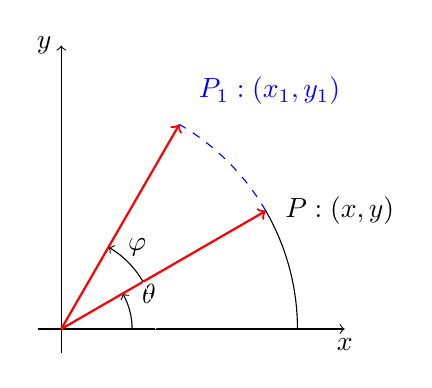
\begin{tikzpicture}[scale=3]
    % \draw[step=.5cm,gray,very thin] (-0.1,-0.1) grid (1.4,1.4);
    \draw[->] (-.1,0) -- (1.2,0)  node[below] {$x$};
    \draw[->] (0,-0.1) -- (0,1.2) node[left] {$y$};
    \draw[]   (1,0) arc (0:30:1) node(P)[label=right:$P:{(x,y)}$]{};
    \draw[->] (3mm,0mm) -- (3mm,0mm) arc (0:30:3mm) node(A)[label=right:$\theta$]{};
    \draw[red, thick, ->] (0,0) --  (P.center);
    
    \draw[white] (4mm,0mm) -- (4mm,0mm) arc (0:30:4mm) node(A){};
    \draw[->] (A.center) arc (30:60:4mm) node[label=right:$\varphi$]{};
    
    \draw[blue, dashed]  (P) arc (30:60:1) node(P1)[label=above right:$P_1:{(x_1,y_1)}$]{};
    
    \draw[red, thick, ->] (0,0) -- (P1.center);    
  \end{tikzpicture}
\end{figure}
这表明经过上述变换,将向量$OP$逆时针旋转$\varphi$角得到向量$OP_1$.


\begin{li}
  求解线性方程组
  $$
  \left\{
    \begin{array}{rcrcrcrcrr}
      2x_1 & - & 2x_2 &   &      & + &  6x_4 & = &-2 \\[0.1cm]
      2x_1 & - &  x_2 & + & 2x_3 & + &  4x_4 & = &-2 \\[0.1cm]
      3x_1 & - &  x_2 & + & 4x_3 & + &  4x_4 & = &-3 \\[0.1cm]
      5x_1 & - & 3x_2 & + &  x_3 & + & 20x_4 & = &-2 
    \end{array}
  \right.
  $$
\end{li}
\begin{jie}
  $$
  \left\{
    \begin{array}{rcrcrcrcrr}
      x_1 & - &  x_2 &   &      & + &  3x_4 & = &-1 \\[0.1cm]
          &  &  x_2 & + & 2x_3 & - &  2x_4 & = &0 \\[0.1cm]
          &  & 2x_2 & + & 4x_3 & - &  5x_4 & = &0 \\[0.1cm]
          &  & 2x_2 & + &  x_3 & + &  5x_4 & = &3 
    \end{array}
  \right.
  $$    
  $$
  \left\{
    \begin{array}{rcrcrcrcrr}
      x_1 & - &  x_2 &   &      & + &  3x_4 & = &-1 \\[0.1cm]
          &  &  x_2 & + & 2x_3 & - &  2x_4 & = &0 \\[0.1cm]
          &  &  &  &  & - &  x_4 & = &0 \\[0.1cm]
          &  &  & - &  3x_3 & + &  9x_4 & = &3 
    \end{array}
  \right.
  $$    
  $$
  \left\{
    \begin{array}{rcrcrcrcrr}
      x_1 & - &  x_2 &   &      & + &  3x_4 & = &-1 \\[0.1cm]
          &  &  x_2 & + & 2x_3 & - &  2x_4 & = &0 \\[0.1cm]
          &  &  & - &  3x_3 & + &  9x_4 & = &3 \\[0.1cm]
          &  &  &  &  & - &  x_4 & = &0 
    \end{array}
  \right.
  $$    
  $$
  \left\{
    \begin{array}{rcrcrcrcrr}
      x_1 & - &  x_2 &   &      & + &  3x_4 & = &-1 \\[0.1cm]
          &  &  x_2 & + & 2x_3 & - &  2x_4 & = &0 \\[0.1cm]
          &  &  &  &  x_3 & - &  3x_4 & = &-1 \\[0.1cm]
          &  &  &  &  &  &  x_4 & = &0 
    \end{array}
  \right.
  $$    
  如此形状的方程组称为\red{阶梯形线性方程组}.
  该方程组可写成矩阵形式
  \begin{figure}[htbp]
    \centering
    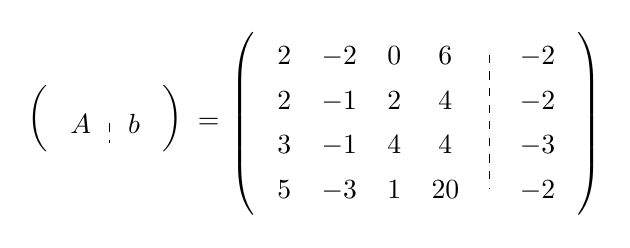
\begin{tikzpicture}
      \matrix(M) [matrix of math nodes,nodes in empty cells,,ampersand replacement=\&,left delimiter=(,right delimiter=)]{
        A \& \& b \\
      };
      \draw[dashed] (M-1-2.north) -- (M-1-2.south);
      \matrix(M1) [right=.1in of M,matrix of math nodes]{
        = \\
      };
      \matrix(MM) [right=.1in of M1,matrix of math nodes,nodes in empty cells,
      column sep=1ex,row sep=.5ex,ampersand replacement=\&,left delimiter=(,right delimiter=)] {
        2 \& -2 \& 0 \&  6 \& \& -2\\
        2 \& -1 \& 2 \&  4 \& \& -2\\
        3 \& -1 \& 4 \&  4 \& \& -3\\
        5 \& -3 \& 1 \& 20 \& \& -2\\
      };
      \draw[dashed] (MM-1-5.north) -- (MM-4-5);
    \end{tikzpicture}
    \caption{增广矩阵}
  \end{figure}
  求解过程可表示为
  \begin{figure}[htbp]
    \centering
    \begin{tikzpicture}          
      \matrix(A) [matrix of math nodes,nodes in empty cells,
      column sep=1ex,row sep=.1ex,ampersand replacement=\&,left delimiter=(,right delimiter=)] {
        A \& \& b \\
      };
      \draw[dashed] (A-1-2.north) -- (A-1-2.south);
      % \end{tikzpicture}
      
      % \begin{tikzpicture}
      \matrix (EQ1) [right=.1in of A,matrix of math nodes]  { 
        \xlongequal[]{\ds r_1 \div 2} \\
      };
      
      \matrix(A1) [right=.1in of EQ1,matrix of math nodes,nodes in empty cells, column sep=1ex,row sep=.1ex,ampersand replacement=\&,left delimiter=(,right delimiter=)] {
        1 \& -1 \& 0 \&  3 \& \& -1\\
        2 \& -1 \& 2 \&  4 \& \& -2\\
        3 \& -1 \& 4 \&  4 \& \& -3\\
        5 \& -3 \& 1 \& 20 \& \& -2\\
      };
      \draw[dashed] (A1-1-5.north) -- (A1-4-5);
      % \end{tikzpicture}

      
      % \begin{tikzpicture}
      
      \matrix(A2) [below=.1in of A1,matrix of math nodes,nodes in empty cells,
      column sep=1ex,row sep=.1ex,ampersand replacement=\&,left delimiter=(,right delimiter=)] {
        1 \& -1 \& 0 \&  3 \& \& -1\\
        0 \&  1 \& 2 \& -2 \& \&  0\\
        0 \&  0 \& 0 \& -1 \& \&  0\\
        0 \&  0 \&-3 \&  9 \& \&  3\\
      };
      \draw[dashed] (A2-1-5.north) -- (A2-4-5);
      \matrix (EQ2) [left=.1in of A2,matrix of math nodes]  { 
        \xlongequal[
        \ds r_3+(-3)\times r_1 \atop 
        \ds r_4+(-5)\times r_1]{\ds r_2+(-2)\times r_1} \\
      };

      % \end{tikzpicture}

      
      % \begin{tikzpicture}
      \matrix(A3) [below=.1in of A2,matrix of math nodes,nodes in empty cells,
      column sep=1ex,row sep=.1ex,ampersand replacement=\&,left delimiter=(,right delimiter=)] {
        1 \& -1 \& 0 \&  3 \& \& -1\\
        0 \&  1 \& 2 \& -2 \& \&  0\\
        0 \&  0 \&-3 \&  9 \& \&  3\\
        0 \&  0 \& 0 \& -1 \& \&  0\\
      };
      \draw[dashed] (A3-1-5.north) -- (A3-4-5);

      \matrix (EQ3) [left=.1in of A3,matrix of math nodes]  { 
        \xlongequal[]{\ds r_3 \leftrightarrow r_4} \\
      };

      
      \matrix(A4) [below=.1in of A3,matrix of math nodes,nodes in empty cells,
      column sep=1ex,row sep=.1ex,ampersand replacement=\&,left delimiter=(,right delimiter=)] {
        1 \& -1 \& 0 \&  3 \& \& -1\\
        0 \&  1 \& 2 \& -2 \& \&  0\\
        0 \&  0 \& 1 \& -3 \& \& -1\\
        0 \&  0 \& 0 \&  1 \& \&  0\\
      };
      \draw[dashed] (A4-1-5.north) -- (A4-4-5);

      \matrix (EQ4) [left=.1in of A4,matrix of math nodes]  { 
        \xlongequal[]{\ds r_3 \div (-3)} \\
      };
    \end{tikzpicture}
  \end{figure}
\end{jie}

\begin{li}
  求解线性方程组
  $$
  \left\{
    \begin{array}{rcrcrcrcrcrr}
      x_1 & - &  x_2 & - &  x_3 &   &       & + & 3x_5 & = &-1 \\[0.1cm]
      2x_1 & - & 2x_2 & - &  x_3 & + &  2x_4 & + & 4x_5 & = &-2 \\[0.1cm]
      3x_1 & - & 3x_2 & - &  x_3 & + &  4x_4 & + & 5x_5 & = &-3 \\[0.1cm]
      x_1 & - &  x_2 & + &  x_3 & + &   x_4 & + & 8x_5 & = & 2 
    \end{array}
  \right.
  $$
\end{li}
\newpage
\begin{jie}
  
  其增广矩阵为
  \begin{figure}[htbp]
    \centering
    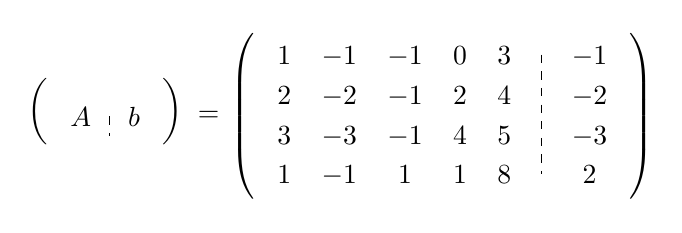
\begin{tikzpicture}
      \matrix(Ab) [matrix of math nodes,nodes in empty cells,,ampersand replacement=\&,left delimiter=(,right delimiter=)]{
        A \& \& b \\
      };
      \draw[dashed] (Ab-1-2.north) -- (Ab-1-2.south);
      \matrix (EQ) [right=.1in of Ab,matrix of math nodes]  { 
        =\\
      };
      \matrix(A) [right=.1in of EQ,matrix of math nodes,nodes in empty cells,   column sep=1ex,row sep=.1ex,ampersand replacement=\&,left delimiter=(,right delimiter=)] {
        1 \& -1 \& -1 \&  0 \& 3 \& \& -1\\
        2 \& -2 \& -1 \&  2 \& 4 \& \& -2\\
        3 \& -3 \& -1 \&  4 \& 5 \& \& -3\\
        1 \& -1 \&  1 \&  1 \& 8 \& \&  2\\
      };
      \draw[dashed] (A-1-6.north) -- (A-4-6);
    \end{tikzpicture}      
  \end{figure}
  
  求解过程可表示为:
  \begin{figure}[htbp]
    \centering
    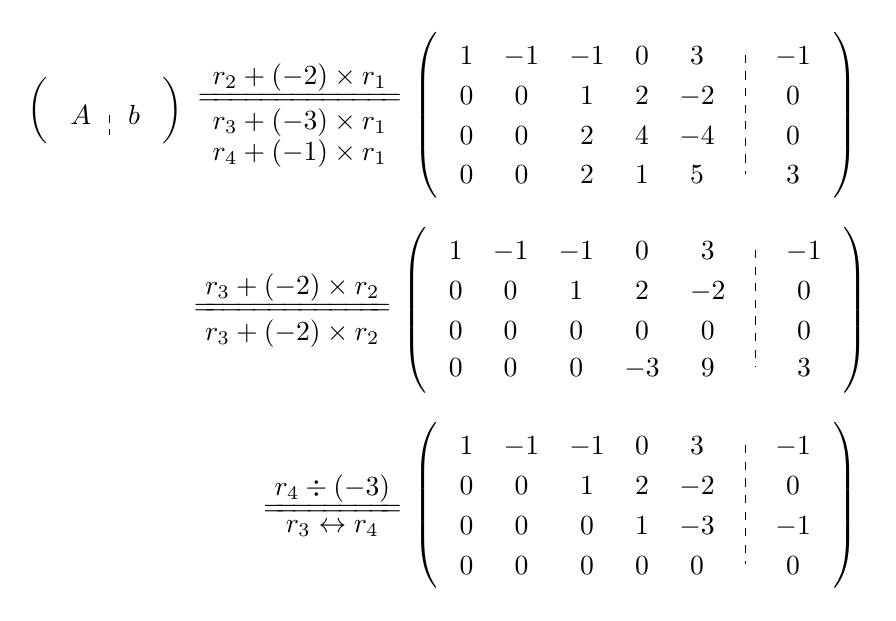
\begin{tikzpicture}
      \matrix(A) [matrix of math nodes,nodes in empty cells,,ampersand replacement=\&,left delimiter=(,right delimiter=)]{
        A \& \& b \\
      };
      \draw[densely dashed] (A-1-2.north) -- (A-1-2.south);
      \matrix (EQ1) [right=.1in of A,matrix of math nodes]  { 
        \xlongequal[\ds r_3+(-3)\times \ds r_1 \atop \ds r_4+(-1)\times r_1]{\ds r_2+(-2)\times r_1}\\
      };        
      \matrix(A1) [right=.1in of EQ1,matrix of math nodes,nodes in empty cells,
      column sep=1ex,row sep=.1ex,ampersand replacement=\&,left delimiter=(,right delimiter=)] {
        1 \& -1 \& -1 \&  0 \& 3 \& \& -1\\
        0 \&  0 \&  1 \&  2 \&-2 \& \&  0\\
        0 \&  0 \&  2 \&  4 \&-4 \& \&  0\\
        0 \&  0 \&  2 \&  1 \& 5 \& \&  3\\
      };
      \draw[dashed] (A1-1-6.north) -- (A1-4-6);

      \matrix(A2) [below=.1in of A1,matrix of math nodes,nodes in empty cells,
      column sep=1ex,row sep=.1ex,ampersand replacement=\&,left delimiter=(,right delimiter=)] {
        1 \& -1 \& -1 \&  0 \& 3 \& \& -1\\
        0 \&  0 \&  1 \&  2 \&-2 \& \&  0\\
        0 \&  0 \&  0 \&  0 \& 0 \& \&  0\\
        0 \&  0 \&  0 \& -3 \& 9 \& \&  3\\
      };
      \draw[dashed] (A2-1-6.north) -- (A2-4-6);
      \matrix (EQ2) [left=.1in of A2,matrix of math nodes]  { 
        \xlongequal[\ds r_3+(-2)\times r_2]{\ds r_3+(-2)\times r_2}\\
      };

      \matrix(A3) [below=.1in of A2,matrix of math nodes,nodes in empty cells,
      column sep=1ex,row sep=.1ex,ampersand replacement=\&,left delimiter=(,right delimiter=)] {
        1 \& -1 \& -1 \&  0 \& 3 \& \& -1\\
        0 \&  0 \&  1 \&  2 \&-2 \& \&  0\\
        0 \&  0 \&  0 \&  1 \& -3 \& \& -1\\
        0 \&  0 \&  0 \&  0 \& 0 \& \&  0\\
      };
      \draw[dashed] (A3-1-6.north) -- (A3-4-6);
      \matrix (EQ3) [left=.1in of A3,matrix of math nodes]  { 
        \xlongequal[\ds r_3 \leftrightarrow r_4]{\ds r_4\div(-3)}\\
      };
    \end{tikzpicture}           
  \end{figure}
  
  该矩阵称为\red{行简化阶梯矩阵},对应的线性方程组为
  $$
  \left\{
    \begin{array}{rcrcrcrcrcrr}
      x_1 & - &  x_2 &   &      &   &       & + & 7x_5 & = & 1 \\[0.1cm]
          &   &     &   &  x_3 &   &     & + & 4x_5 & = & 2 \\[0.1cm]
          &   &   &   &    &   &   x_4 & - & 3x_5 & = &-1
    \end{array}
  \right.
  $$
  \begin{zhu*}
    该方程组有$5$个未知量,其中$x_1,x_3,x_4$为\red{基本未知量},$x_2,x_5$为\red{自由未知量}。
  \end{zhu*}

  任取$x_2=k_1, x_5=k_2$,可得线性方程组的全部解
  $$
  \left\{
    \begin{array}{ccl}
      x_1 &=& 1+k_1-7k_2, \\[0.1cm]      
      x_2 &=& k_1, \\[0.1cm]
      x_3 &=& 2-4k_2, \\[0.1cm]
      x_4 &=& -1+3k_2,\\[0.1cm]
      x_5 &=& k_2.
    \end{array}
  \right.
  $$

\end{jie}

\begin{li}
  解线性方程组
  $$
  \left\{
    \begin{array}{rcrcrcr}
      x_1 & + & x_2 & + &  x_3 & = & 1, \\[0.1cm]
      x_1 & + &2x_2 & - & 5x_3 & = & 2, \\[0.1cm]
      2x_1 & + &3x_2 & - & 4x_3 & = & 5.
    \end{array}
  \right.
  $$
\end{li}
\newpage
\begin{jie}
  
  \begin{figure}[htbp]
    \centering
    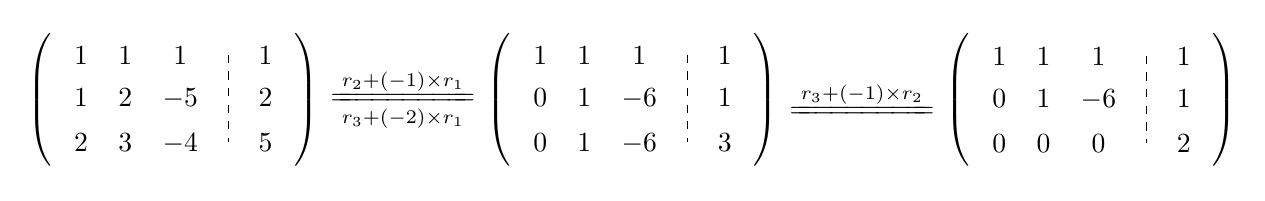
\begin{tikzpicture}        
      \matrix(Ab) [matrix of math nodes,nodes in empty cells,
      column sep=1ex,row sep=.5ex,ampersand replacement=\&,left delimiter=(,right delimiter=)] {
        1 \&  1 \&  1 \& \&  1\\
        1 \&  2 \& -5 \& \&  2\\
        2 \&  3 \& -4 \& \&  5\\
      };
      \draw[dashed] (Ab-1-4.north) -- (Ab-3-4);
      
      \matrix (EQ1) [right=.1in of Ab,matrix of math nodes]  { 
        \xlongequal[r_3+ (-2)\times r_1]{r_2+ (-1)\times r_1}\\
      };

      \matrix(Ab1) [right=.1in of EQ1,matrix of math nodes,nodes in empty cells, column sep=1ex,row sep=.5ex,ampersand replacement=\&,left delimiter=(,right delimiter=)] {
        1 \&  1 \&  1 \& \&  1\\
        0 \&  1 \& -6 \& \&  1\\
        0 \&  1 \& -6 \& \&  3\\
      };
      \draw[dashed] (Ab1-1-4.north) -- (Ab1-3-4);

      \matrix (EQ2) [right=.1in of Ab1,matrix of math nodes]  { 
        \xlongequal[]{r_3+ (-1)\times r_2}\\
      };
      \matrix(Ab2) [right=.1in of EQ2,matrix of math nodes,nodes in empty cells,column sep=1ex,row sep=.5ex,ampersand replacement=\&,left delimiter=(,right delimiter=)] {
        1 \&  1 \&  1 \& \&  1\\
        0 \&  1 \& -6 \& \&  1\\
        0 \&  0 \&  0 \& \&  2\\
      };
      \draw[dashed] (Ab2-1-4.north) -- (Ab2-3-4);        
    \end{tikzpicture}
  \end{figure}
  
  由第三行可以看出,该线性方程组无解。
\end{jie}

\begin{itemize}
\item 含有矛盾方程而无解的方程组称为\red{不相容方程组};
\item 有解的方程组称为\red{相容方程组};
\item \red{多余方程}。
\end{itemize}

对于一般的线性方程组
$$
\left\{
  \begin{array}{c}
    a_{11}x_1 + a_{12}x_2 + \cd + a_{1n}x_n = b_1\\[0.2cm]
    a_{21}x_1 + a_{22}x_2 + \cd + a_{2n}x_n = b_2\\[0.2cm]
    \vd\\[0.2cm]
    a_{m1}x_1 + a_{m2}x_2 + \cd + a_{mn}x_n = b_m
  \end{array}
\right.
$$

其增广矩阵为
\begin{figure}[htbp]
  \centering
  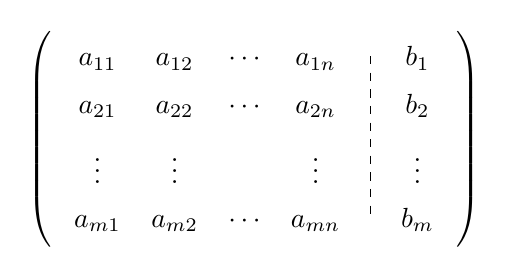
\begin{tikzpicture}
    \matrix(MM) [matrix of math nodes,nodes in empty cells,
    column sep=1ex,row sep=.5ex,ampersand replacement=\&,left delimiter=(,right delimiter=)] {
      a_{11} \&  a_{12} \&  \cd \& a_{1n} \& \&  b_1\\
      a_{21} \&  a_{22} \&  \cd \& a_{2n} \& \&  b_2\\
      \vd   \&  \vd   \&      \&  \vd  \& \& \vd \\
      a_{m1} \&  a_{m2} \&  \cd \& a_{mn} \& \&  b_m\\
    };
    \draw[dashed] (MM-1-5.north) -- (MM-4-5);        
  \end{tikzpicture}      
\end{figure}
对于以上增广矩阵,总是可以经过一系列的变换将其化成
\begin{figure}[htbp]
  \centering
  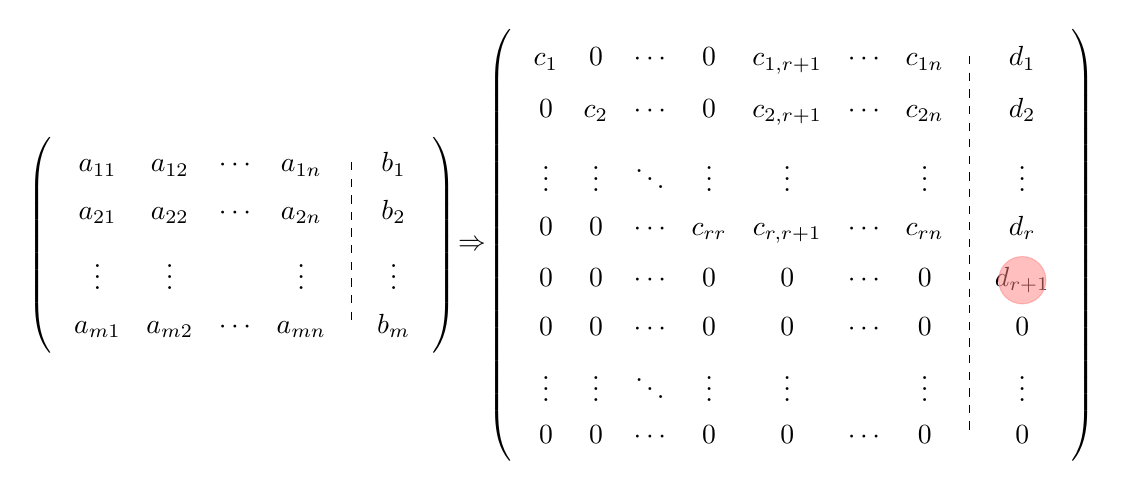
\begin{tikzpicture}
    \matrix(MM) [matrix of math nodes,nodes in empty cells,
    column sep=0.6ex,row sep=.5ex,ampersand replacement=\&,left delimiter=(,right delimiter=)] {
      a_{11} \&  a_{12} \&  \cd \& a_{1n} \& \&  b_1\\
      a_{21} \&  a_{22} \&  \cd \& a_{2n} \& \&  b_2\\
      \vd   \&  \vd   \&      \&  \vd  \& \& \vd \\
      a_{m1} \&  a_{m2} \&  \cd \& a_{mn} \& \&  b_m\\
    };
    \draw[dashed] (MM-1-5.north) -- (MM-4-5);
    
    \matrix (M2) [right=.05in of MM,matrix of math nodes]  { 
      \Rightarrow\\
    };
    
    \matrix(MM) [right=.05in of M2,matrix of math nodes,nodes in empty cells,
    column sep=0.6ex,row sep=.5ex,ampersand replacement=\&,left delimiter=(,right delimiter=)] {
      c_1 \&   0 \& \cd \&  0 \& c_{1,r+1} \& \cd \& c_{1n} \& \& d_1\\
      0   \& c_2 \& \cd \&  0 \& c_{2,r+1} \& \cd \& c_{2n} \& \& d_2\\
      \vd \& \vd \& \dd \&\vd \& \vd     \&     \& \vd   \& \& \vd\\
      0   \&  0  \& \cd \& c_{rr} \& c_{r,r+1} \& \cd \& c_{rn} \& \& d_r\\
      0   \&  0  \& \cd \& 0 \& 0 \& \cd \& 0 \&  \& d_{r+1}\\
      0   \&  0  \& \cd \& 0 \& 0 \& \cd \& 0 \&  \& 0\\          
      \vd \& \vd \& \dd \&\vd \& \vd     \&     \& \vd   \& \& \vd\\
      0   \&  0  \& \cd \& 0 \& 0 \& \cd \& 0 \&  \& 0\\
    };
    \draw[dashed] (MM-1-8.north) -- (MM-8-8);
    \filldraw[opacity=0.5,red!50] (MM-5-9) circle (0.3cm);
  \end{tikzpicture}      
\end{figure}
其中$c_{ii}=1~(i=1,2,\cd,r)$。对应线性方程组解的情况如下:   
\begin{itemize}
\item[1] 线性方程组有解$ \Leftrightarrow \red{d_{r+1}=0}$;\\[0.3cm]
\item[2] 在有解的情况下:
  \begin{itemize}
  \item 当$r=n$时,有唯一解$x_1=d_1,~x_2=d_2,~\cd,~x_n=d_n$;
  \item 当$r<n$时,有无穷多解
    $$
    \left\{
      \begin{array}{ccl}
        x_1 &=& d_1 - c_{1,r+1}k_1 - \cd - c_{1n}k_{n-r}, \\[0.1cm]
        x_2 &=& d_2 - c_{2,r+1}k_1 - \cd - c_{2n}k_{n-r}, \\[0.1cm]
        \vd & & \vd \\[0.1cm]
        x_r &=& d_r - c_{r,r+1}k_1 - \cd - c_{rn}k_{n-r}, \\[0.1cm]
        x_{r+1} &=& k_1, \\[0.1cm]
        \vd && \vd \\[0.1cm]
        x_{n} &=& k_{n-r}.
      \end{array}
    \right.
    $$
  \end{itemize}
\end{itemize}

  %%%% 
\section{矩阵的计算}
\subsection{矩阵的加法}
\begin{frame}
  \begin{footnotesize}
    
    \begin{block}{矩阵的加法}
      设有两个$m\times n$矩阵$\A=(a_{ij})$和$\B=(b_{ij})$,则矩阵$\A$与$\B$之和记为$\A+\B$,规定为
      $$
      \A + \B = 
      \left(
        \begin{array}{cccc}
          a_{11} + b_{11}  & a_{12} + b_{12}  & \cd & a_{1n} + b_{1n}  \\[0.2cm]
          a_{21} + b_{21}  & a_{22} + b_{22}  & \cd & a_{2n} + b_{2n}  \\[0.2cm]
          \cd            & \cd            &     & \cd            \\[0.2cm]
          a_{n1} + b_{n1}  & a_{n2} + b_{n2}  & \cd & a_{nn} + b_{nn}  
        \end{array}
      \right)
      $$
    \end{block}
    \pause
    \begin{block}{注}
      \red{只有当两个矩阵同型时才能进行加法运算。}
    \end{block}

    


  \end{footnotesize}
\end{frame}


\begin{frame}
  \begin{footnotesize}
    \begin{block}{矩阵加法运算律}
      \begin{itemize}
      \item[(i)] $\A + \B = \B + \A$\\[0.2cm]
      \item[(ii)] $(\A + \B) + \C = \A + (\B + \C)$ 
      \end{itemize}
    \end{block}

    \vspace{0.1in}
    \pause 
    设$\A = (a_{ij})$,称
    $$
    -\A = (-a_{ij}),
    $$
    为$\A$的负矩阵,显然有
    $$
    \A + (-\A) = \mathbf{0}.
    $$
    由此规定矩阵的减法为
    $$
    \A - \B = \A + (-\B).
    $$
  \end{footnotesize}
\end{frame}

\subsection{矩阵的数乘}
\begin{frame}
  \begin{footnotesize}
    \begin{block}{矩阵的数乘}
      数$k$与矩阵$\A$的乘积记作$k \A$或$\A k$,规定为
      $$
      k \A = 
      \left(
        \begin{array}{cccc}
          k a_{11}   & k a_{12}   & \cd & k a_{1n}  \\[0.2cm]
          k a_{21}   & k a_{22}   & \cd & k a_{2n}  \\[0.2cm]
          \cd     & \cd     &     & \cd    \\[0.2cm]
          k a_{m1}   & k a_{m2}   & \cd & k a_{mn}  
        \end{array}
      \right)
      $$
    \end{block}
    \pause 
    \begin{block}{注}
      \red{用数$k$乘一个矩阵,需要把数$k$乘矩阵的每一个元素,这与行列式的数乘性质不同。}
    \end{block}
  \end{footnotesize}
\end{frame}


\begin{frame}
  \begin{footnotesize}
    \begin{block}{矩阵数乘运算律}
      \begin{itemize}
      \item[(i)] $(k l)\A =  k(l \A)$\\[0.2cm]
      \item[(ii)] $(k + l) \A  = k \A + l \A$\\[0.2cm]
      \item[(iii)] $k (\A + \B)  = k \A + k \B$
      \end{itemize}
    \end{block}
    \pause 
    \purple{矩阵加法与矩阵数乘统称为矩阵的线性运算}
  \end{footnotesize}
\end{frame}


\subsection{矩阵的乘法}
\begin{frame}
  \begin{footnotesize}
    设有两个线性变换
    \begin{equation}\label{lt1}
      \left\{
        \begin{array}{l}
          y_1 = a_{11} x_1 + a_{12} x_2 + a_{13} x_3, \\[0.2cm]
          y_2 = a_{21} x_1 + a_{22} x_2 + a_{23} x_3,
        \end{array}
      \right.
    \end{equation}
    \pause
    \begin{equation}\label{lt2}
      \left\{
        \begin{array}{l}
          x_1 = b_{11} t_1 + b_{12} t_2 , \\[0.2cm]
          x_2 = b_{21} t_1 + b_{22} t_2 , \\[0.2cm]
          x_3 = b_{31} t_1 + b_{32} t_2 , 
        \end{array}
      \right.
    \end{equation}
    \pause
    若想求从$t_1, t_2$到$y_1, y_2$的线性变换,可将(\ref{lt2})代入(\ref{lt1}),便得
    \begin{equation}\label{lt3}
      \left\{
        \begin{array}{l}
          y_1 = (a_{11}b_{11} + a_{12}b_{21} + a_{13}b_{31}) t_1 + (a_{11}b_{12} + a_{12}b_{22} + a_{13}b_{32})t_2, \\[0.2cm]
          y_2 = (a_{21}b_{11} + a_{22}b_{21} + a_{23}b_{31}) t_1 + (a_{21}b_{12} + a_{22}b_{22} + a_{23}b_{32})t_2.
        \end{array}
      \right.
    \end{equation}
    \pause
    \red{线性变换(\ref{lt3})可看成是先作线性变换(\ref{lt2})再作线性变换(\ref{lt1})的结果}。
  \end{footnotesize}
\end{frame}

\begin{frame}
  \begin{footnotesize}
    把线性变换(\ref{lt3})叫做线性变换(\ref{lt1})和(\ref{lt2})的乘积,
    相应地把线性变换(\ref{lt3})对应的矩阵定义为线性变换(\ref{lt1})与(\ref{lt2})所对应矩阵的乘积,即
    $$
    \begin{array}{ll}
      & \left(
        \begin{array}{lll}
          a_{11} & a_{12} & a_{13}\\[0.1cm]
          a_{21} & a_{22} & a_{23}
        \end{array}
                            \right)
                            \left(
                            \begin{array}{ll}
                              b_{11} & b_{12} \\[0.1cm]
                              b_{21} & b_{22} \\[0.1cm]
                              b_{31} & b_{32} 
                            \end{array}
                                       \right) \\[0.8cm]
      = & \left(
          \begin{array}{cc}
            a_{11}b_{11} + a_{12}b_{21} + a_{13}b_{31}  &  a_{11}b_{12} + a_{12}b_{22} + a_{13}b_{32} \\[0.1cm]
            a_{21}b_{11} + a_{22}b_{21} + a_{23}b_{31}  &  a_{21}b_{12} + a_{22}b_{22} + a_{23}b_{32}
          \end{array}
                                                          \right)
    \end{array}
    $$
  \end{footnotesize}
\end{frame}

\begin{frame}
  \begin{footnotesize}
    \begin{block}{矩阵乘法}
      设$A$为$m\times n$矩阵,$B$为$n\times s$矩阵,即
      $$
      A = \left(
        \begin{array}{cccc}
          a_{11} & a_{12} & \cd & a_{1n}\\
          a_{21} & a_{22} & \cd & a_{2n}\\
          \vd   & \vd   &     & \vd \\
          a_{m1} & a_{m2} & \cd & a_{mn}
        \end{array}
      \right), ~~
      B = \left(
        \begin{array}{cccc}
          b_{11} & b_{12} & \cd & b_{1s}\\
          b_{21} & b_{22} & \cd & b_{2s}\\
          \vd   & \vd   &     & \vd \\
          b_{n1} & b_{n2} & \cd & b_{ns}
        \end{array}
      \right)
      $$
      则$A$与$B$之乘积$AB$(记为$C=(c_{ij})$)为$m\times s$矩阵,且
      $$
      c_{ij} = c_{i1}b_{1j} + c_{i2}b_{2j} + \cd + c_{in}b_{nj} = \sum_{k=1}^na_{ik}b_{kj}.
      $$
    \end{block}
    \pause 
    \begin{block}{注}
      两个矩阵$A$与$B$相乘有意义的前提是\red{$A$的列数等于$B$的行数}。
    \end{block}
  \end{footnotesize}
\end{frame}


\begin{frame}
  % l' unite
  \newcommand{\myunit}{0.5 cm}
  \tikzset{
    node style sp/.style={draw,circle,minimum size=\myunit},
    node style ge/.style={circle,minimum size=\myunit},
    arrow style mul/.style={draw,sloped,midway,fill=white},
    arrow style plus/.style={midway,sloped,fill=white},
  }
  
  \begin{tikzpicture}[scale=0.5,>=latex]
    % les matrices
    \matrix (A) [matrix of math nodes,%
    nodes = {node style ge},%
    ampersand replacement=\&,
    left delimiter  = (,%
    right delimiter = )] at (0,0)   {%
      a_{11} \& a_{12} \& \ldots \& a_{1n}  \\
      \blue{a_{21}}  \& \blue{a_{22}}; \& \ldots%
      \& \blue{a_{2n}} \\
      \vdots \& \vdots \& \ddots \& \vdots  \\
      a_{m1} \& a_{m2} \& \ldots \& a_{mn}  \\
    };
    \pause 
    % \node [draw,below=1pt] at (A.south) { 
    % $A$ : \textcolor{red}{$n$ rows} $p$ columns};

    \matrix (B) [matrix of math nodes,%
    % nodes = {node style ge},%
    ampersand replacement=\&,
    left delimiter  = (,%
    right delimiter =)] at (20*\myunit,18*\myunit){%
      b_{11} \& \blue{b_{12}}%
      \& \ldots \& b_{1s}  \\
      b_{21} \& \blue{b_{22}}%
      \& \ldots \& b_{2s}  \\
      \vdots \& \vdots \& \ddots \& \vdots  \\
      b_{n1} \& \blue{b_{n2}}%
      \& \ldots \& b_{ns}  \\
    };
    \pause
    %% \node [draw,above=10pt] at (B.north) { 
    %% $B$ : $p$ rows \textcolor{red}{$q$ columns}
    %% };
    %   matrice 
    \matrix (C) [matrix of math nodes,%
    nodes = {node style ge},%
    ampersand replacement=\&,
    left delimiter  = (,%
    right delimiter = )] at (20*\myunit,0) {%
      c_{11} \& c_{12} \& \ldots \& c_{1s} \\
      c_{21} \& \red{c_{22}}%
      \& \ldots \& c_{2s} \\
      \vdots \& \vdots \& \ddots \& \vdots \\
      c_{m1} \& c_{m2} \& \ldots \& c_{ms} \\
    };
    \pause 
    % les fleches
    \draw[<->,red](A-2-1) to[in=180,out=90]
    node[arrow style mul] (x) {$a_{21}\times b_{12}$} (B-1-2);
    \pause 
    \draw[<->,red](A-2-2) to[in=180,out=90]
    node[arrow style mul] (y) {$a_{22}\times b_{22}$} (B-2-2);
    \pause 
    \draw[<->,red](A-2-4) to[in=180,out=90]
    node[arrow style mul] (z) {$a_{2n}\times b_{n2}$} (B-4-2);
    \pause 
    \draw[red,->] (x) to node[arrow style plus] {$+$} (y)%
    to node[arrow style plus] {$+\raisebox{.5ex}{\ldots}+$} (z)%
    to (C-2-2.north west);
    \pause 
    \draw[blue] (A-2-1.north) -- (C-2-2.north);
    \draw[blue] (A-2-1.south) -- (C-2-2.south);

    \draw[blue] (B-1-2.west)  -- (C-2-2.west);
    \draw[blue] (B-1-2.east)  -- (C-2-2.east);

    %% \node [draw,below=10pt] at (C.south) 
    %% {$ C=A\times B$ : \textcolor{red}{$n$ rows}  \textcolor{red}{$q$ columns}};

  \end{tikzpicture}

\end{frame}

\begin{frame}
  \begin{footnotesize}
    \begin{exampleblock}{例1}
      求矩阵
      $
      \A = \left(
        \begin{array}{rrrr}
          1&2&-1\\
          -1&3&4\\
          1&1&1
        \end{array}
      \right)
      $
      与
      $
      \B = \left(
        \begin{array}{rrrr}
          5&6\\
          -5&-6\\
          6&0
        \end{array}
      \right)
      $
      的乘积$\A\B$
    \end{exampleblock}
    \pause
    \textbf{解:}
    $$
    \begin{array}{cl}
      \A\B &\pause = \left(
             \begin{array}{ccc}
               1\times5 + 2\times(-5) + (-1)\times6 &
                                                      1\times6 + 2\times(-6) + (-1)\times0 \\[0.1cm]
               (-1)\times5 + 3\times(-5) +    4\times6 &
                                                         (-1)\times6 + 3\times(-6) +    4\times0 \\[0.1cm]
               1\times5 + 1\times(-5) +    1\times6 &
                                                      1\times6 + 1\times(-6) +    1\times0 
             \end{array}
                                                      \right) \\[0.3in]
           &\pause =\left(
             \begin{array}{rr}
               -11 & -6\\
               4 & -24\\
               6 & 0
             \end{array}
                   \right)   
    \end{array}
    $$
  \end{footnotesize}
\end{frame}

\begin{frame}
  \begin{footnotesize}
    \begin{exampleblock}{例2}
      设
      $$
      \A = \left(
        \begin{array}{c}
          a_1\\
          a_2\\
          \vd\\
          a_n
        \end{array}
      \right), ~~
      \B = \left(
        \begin{array}{cccc}
          b_1 & b_2 & \cd & b_n
        \end{array}
      \right)
      $$
      计算$\A\B$与$\B\A$.
    \end{exampleblock}
    \textbf{解:}
    $$
    \A\B = \left(
      \begin{array}{c}
        a_1\\
        a_2\\
        \vd\\
        a_n
      \end{array}
    \right)\left(
      \begin{array}{cccc}
        b_1 & b_2 & \cd & b_n
      \end{array}
    \right)\pause 
    = \left(
      \begin{array}{cccc}
        a_1b_1 & a_1b_2 & \cd & a_1b_n\\
        a_2b_1 & a_2b_2 & \cd & a_2b_n\\
        \vd & \vd & & \vd\\
        a_nb_1 & a_nb_2 & \cd & a_nb_n
      \end{array}
    \right)
    $$ \pause 
    $$
    \B\A = \left(
      \begin{array}{cccc}
        b_1 & b_2 & \cd & b_n
      \end{array}
    \right)\left(
      \begin{array}{c}
        a_1\\
        a_2\\
        \vd\\
        a_n
      \end{array}
    \right) \pause 
    = a_1b_1+a_2b_2+\cd+a_nb_n.
    $$
  \end{footnotesize}
\end{frame}

\begin{frame}
  \begin{footnotesize}
    \begin{exampleblock}{例3}
      设
      $$
      \A = \left(
        \begin{array}{cc}
          a & a\\
          -a & -a
        \end{array}
      \right), ~
      \B = \left(
        \begin{array}{cc}
          b & -b\\
          -b & b
        \end{array}
      \right),~
      \C = \left(
        \begin{array}{cc}
          -1 & 1\\
          1 & -1
        \end{array}
      \right)
      $$
      计算$\A\B, ~\A\C$和$\B\A$.
    \end{exampleblock}
    \pause
    \textbf{解:}
    $$
    \A\B = \A\C = \left(
      \begin{array}{cc}
        0 & 0\\
        0 & 0
      \end{array}
    \right)
    $$\pause
    $$
    \B\A = \left(
      \begin{array}{cc}
        2ab & 2ab\\
        -2ab & -2ab
      \end{array}
    \right)
    $$      
  \end{footnotesize}
\end{frame}


\begin{frame}
  \begin{footnotesize}
    由以上例题可以看出一些结论:\pause 
    \begin{itemize}
    \item[1] 矩阵乘法不满足交换律。\\[0.2cm] \pause 
    \item[] 若$\A\B\ne\B\A$,则称\red{$\A$与$\B$不可交换}。\\[0.2cm] \pause 
    \item[] 若$\A\B=\B\A$,则称\red{$\A$与$\B$可交换}。  \\[0.4cm] \pause 
    \item[2] $\A\B=\zero ~\nRightarrow~ \A = \zero \mbox{或} \B = \zero$\\[0.2cm] \pause 
    \item[]  $\A\ne\zero\mbox{且} \B\ne\zero ~\xLongrightarrow[]{\mbox{有可能}}~ \A \B= \zero$\\[0.4cm] \pause
    \item[3] 矩阵乘法不满足消去律,即当$\A\ne\zero$时,
      $$
      \A\B=\A\C ~\nRightarrow~ \B=\C
      $$\\[0.2cm] \pause 
    \item[]当$\A$为非奇异矩阵,即$|\A|\ne 0$时,
      $$
      \A\B=\zero ~\Rightarrow~ \B = \zero; ~~~
      \A\B=\A\C ~\Rightarrow~ \B = \C.
      $$
    \end{itemize}
  \end{footnotesize}
\end{frame}


\begin{frame}
  \begin{footnotesize}
    \begin{block}{矩阵乘法运算律}
      \begin{itemize}
      \item[(i)] 结合律
      \item[] $$ (\A\B)\C = \A(\B\C)$$
      \item[(ii)] 数乘结合律
      \item[] $$ k(\A\B) = (k\A)\B = \A(k\B)$$
      \item[(iii)] 左结合律
      \item[] $$ \A(\B+\C) = \A\B+\A\C$$
      \item[] 右结合律
      \item[] $$ (\B+\C)\A = \B\A+\C\A$$
        
      \end{itemize}
    \end{block}
  \end{footnotesize}
\end{frame}

\subsection{一些特殊矩阵及其运算}
\begin{frame}
  \begin{footnotesize}
    \begin{block}{单位矩阵与数量矩阵}
      \begin{itemize}
      \item[1] 主对角元全为1,其余元素全为零的$n$阶方阵,称为$n$阶\red{单位矩阵},记为$\II_n, \II, \E$
        $$
        \II_n = \left(
          \begin{array}{cccc}
            1 & & &\\
              & 1 & & \\
              & & \dd & \\
              & & & 1
          \end{array}
        \right)
        $$\pause 
      \item[2] 主对角元全为非零数$k$,其余元素全为零的$n$阶方阵,称为$n$阶\red{数量矩阵},记为$k\II_n, k\II, k\E$
        $$
        k\II_n = \left(
          \begin{array}{cccc}
            k & & &\\
              & k & & \\
              & & \dd & \\
              & & & k
          \end{array}
        \right)~(k\ne 0)
        $$
      \end{itemize}
    \end{block}
    \pause 
    \begin{block}{注}
      \begin{itemize}
      \item[1] \red{单位阵在矩阵乘法中的作用相当于数$1$在数的乘法中的作用。}\\ \pause 
      \item[2] 
        $$
        (k\II) \A = k(\II\A) = k\A, ~~
        \A(k\II) = k(\A\II) = k\A.
        $$
      \end{itemize}
    \end{block}
  \end{footnotesize}
\end{frame}


\begin{frame}
  \begin{footnotesize}
    \begin{block}{对角矩阵}
      非对角元皆为零的$n$阶方阵称为$n$阶\red{对角矩阵},记作$\LLambda$,即
      $$
      \LLambda = \left(
        \begin{array}{cccc}
          \lambda_1 & & &\\
                    & \lambda_2 & & \\
                    & & \dd & \\
                    & & & \lambda_n
        \end{array}
      \right)
      $$
      或记作$\mathrm{diag}(\lambda_1,\lambda_2,\cd,\lambda_n)$.
    \end{block}
  \end{footnotesize}
\end{frame}


\begin{frame}
  \begin{footnotesize}
    \begin{block}{注}
      \begin{itemize}
      \item[1] 用对角阵$\LLambda$左乘$\A$,就是用$\lambda_i(i=1,\cd,n)$乘$\A$中第$i$行的每个元素;
        \pause 
      \item[]
        \begin{scriptsize}
          $$
          \left(
            \begin{array}{cccc}
              \lambda_1 & & &\\
                        & \lambda_2 & & \\
                        & & \dd & \\
                        & & & \lambda_n
            \end{array}
          \right)
          \left(
            \begin{array}{cccc}
              a_{11} & a_{12} & \cd & a_{1n}\\
              a_{21} & a_{22} & \cd & a_{2n}\\
              \vd & \vd &  & \vd\\
              a_{n1} & a_{n2} & \cd & a_{nn}
            \end{array}
          \right) = 
          \left(
            \begin{array}{cccc}
              \lambda_1 a_{11} & \lambda_1a_{12} & \cd & \lambda_1a_{1n}\\
              \lambda_2a_{21} & \lambda_2a_{22} & \cd & \lambda_2a_{2n}\\
              \vd & \vd &  & \vd\\
              \lambda_na_{n1} & \lambda_na_{n2} & \cd & \lambda_na_{nn}
            \end{array}
          \right)
          $$

        \end{scriptsize}
        \pause 
      \item[2] 用对角阵$\LLambda$右乘$\A$,就是用$\lambda_i(i=1,\cd,n)$乘$\A$中第$i$列的每个元素;
        \pause 
      \item[]
        \begin{scriptsize}
          $$
          \left(
            \begin{array}{cccc}
              a_{11} & a_{12} & \cd & a_{1n}\\
              a_{21} & a_{22} & \cd & a_{2n}\\
              \vd & \vd &  & \vd\\
              a_{n1} & a_{n2} & \cd & a_{nn}
            \end{array}
          \right)  
          \left(
            \begin{array}{cccc}
              \lambda_1 & & &\\
                        & \lambda_2 & & \\
                        & & \dd & \\
                        & & & \lambda_n
            \end{array}
          \right)
          = 
          \left(
            \begin{array}{cccc}
              \lambda_1a_{11} & \lambda_2a_{12} & \cd & \lambda_na_{1n}\\
              \lambda_1a_{21} & \lambda_2a_{22} & \cd & \lambda_na_{2n}\\
              \vd & \vd &  & \vd\\
              \lambda_1a_{n1} & \lambda_2a_{n2} & \cd & \lambda_na_{nn}
            \end{array}
          \right)
          $$

        \end{scriptsize}
      \end{itemize}
    \end{block}
  \end{footnotesize}
\end{frame}


\begin{frame}
  \begin{footnotesize}
    \begin{block}{三角矩阵}
      \begin{itemize}
      \item[1] 主对角线以上的元素全为零的$n$阶方阵称为\red{上三角矩阵}($a_{ij}=0, ~i>j$)
        $$
        \left(
          \begin{array}{cccc}
            a_{11} & a_{12} & \cd & a_{1n} \\
                   & a_{22} & \cd & a_{2n} \\
                   &       & \dd & \vd   \\
                   &       &     & a_{nn}
          \end{array}
        \right)
        $$
      \item[2] 主对角线以下的元素全为零的$n$阶方阵称为\red{下三角矩阵}($a_{ij}=0, ~i<j$)
        $$
        \left(
          \begin{array}{cccc}
            a_{11} &       &     &       \\
            a_{21} & a_{22} &     &  \\
            \vd   & \vd   & \dd &    \\
            a_{n1} & a_{n2} & \cd & a_{nn}
          \end{array}
        \right)
        $$
      \end{itemize}
    \end{block}
  \end{footnotesize}
\end{frame}

\begin{frame}
  \begin{footnotesize}
    \begin{exampleblock}{例4}
      证明:两个上三角矩阵的乘积仍为上三角矩阵。
    \end{exampleblock}
    \proofname
    设
    $$
    \A = \left(
      \begin{array}{cccc}
        a_{11} & a_{12} & \cd & a_{1n} \\
               & a_{22} & \cd & a_{2n} \\
               &       & \dd & \vd   \\
               &       &     & a_{nn}
      \end{array}
    \right), ~     \B = \left(
      \begin{array}{cccc}
        b_{11} & b_{12} & \cd & b_{1n} \\
               & b_{22} & \cd & b_{2n} \\
               &       & \dd & \vd   \\
               &       &     & b_{nn}
      \end{array}
    \right)
    $$
    \pause 
    令$\C = \A\B = (c_{ij})$,
    则当$i>j$时,
    $$
    c_{ij} = \sum_{k=1}^n a_{ik}b_{kj}  \pause 
    = \sum_{k=1}^{i-1} a_{ik}b_{kj}  + \sum_{k=i}^n a_{ik}b_{kj} \pause 
    = \sum_{k=1}^{i-1} \red{\underbrace{a_{ik}}_{\Downarrow\atop0}}b_{kj}  
    + \sum_{k=i}^n a_{ik}\red{\underbrace{b_{kj}}_{\Downarrow\atop0}} \pause = 0.
    $$
    \pause 
    \begin{block}{注}
      两个下三角矩阵的乘积仍是下三角矩阵。
    \end{block}
  \end{footnotesize}
\end{frame}


\begin{frame}
  \begin{footnotesize}
    设线性方程组
    $$
    \left\{
      \begin{array}{c}
        a_{11}x_1 + a_{12}x_2 + a_{1n}x_n = b_1, \\[0.2cm]
        a_{21}x_1 + a_{22}x_2 + a_{2n}x_n = b_2, \\[0.2cm]
        \vd \\[0.2cm]
        a_{m1}x_1 + a_{m2}x_2 + a_{mn}x_n = b_m.
      \end{array}
    \right.
    $$
    \pause
    第$i$个方程可表示为
    $$
    \left(
      \begin{array}{cccc}
        a_{i1} & a_{i2} & \cd &  a_{in}
      \end{array}
    \right)
    \left(
      \begin{array}{c}
        x_{1} \\
        x_{2} \\
        \cd   \\
        x_{n}
      \end{array}
    \right) = b_i, \quad i=1,2,\cd,n.
    $$\pause 
    因此上述线性方程组可表示为
    $$
    \underbrace{
      \left(
        \begin{array}{cccc}
          a_{11} & a_{12} & \cd &  a_{1n} \\[0.1cm]
          a_{21} & a_{22} & \cd &  a_{2n} \\[0.1cm]
          \vd   & \vd   &     & \vd \\[0.1cm]
          a_{n1} & a_{n2} & \cd &  a_{nn} \\[0.1cm]
        \end{array}
      \right)
    }_{\red{\A}}
    \underbrace{
      \left(
        \begin{array}{c}
          x_{1} \\[0.1cm]
          x_{2} \\[0.1cm]
          \vd  \\[0.1cm]
          x_{n}
        \end{array}
      \right)
    }_{\red{\xx}}
    =     
    \underbrace{
      \left(
        \begin{array}{c}
          b_{1} \\[0.1cm]
          b_{2} \\[0.1cm]
          \vd  \\[0.1cm]
          b_{n}
        \end{array}
      \right)
    }_{\red{\bb}},  
    \pause \quad \red{\A\xx=\bb}.
    $$
  \end{footnotesize}
\end{frame}


\begin{frame}
  \begin{footnotesize}
    \begin{block}{定理}
      设$\A,\B$是两个$n$阶方阵,则
      $$
      |\A\B| = |\A||\B|.
      $$
    \end{block}
    \pause 
    \proofname
    设$\A=(a_{ij})_{n\times n}, ~\B=(b_{ij})_{n\times n}$,则
    $$
    |\A||\B| = \left|
      \begin{array}{cccccccc}
        a_{11} & a_{12} & \cd &  a_{1n} & 0 & 0 & \cd & 0\\
        a_{21} & a_{22} & \cd &  a_{2n} & 0 & 0 & \cd & 0\\
        \vd   & \vd   &     & \vd    & \vd & \vd & & \vd\\
        a_{n1} & a_{n2} & \cd &  a_{nn} & 0 & 0 & \cd & 0\\
        -1    & 0     & \cd &   0    & b_{11} & b_{12} & \cd & b_{1n} \\
        0 & -1 & \cd & 0& b_{21} & b_{22} & \cd & b_{2n} \\
        \vd&\vd & & \vd &  \vd  &\vd &  & \vd   \\
        0 & 0 & \cd & -1 & b_{n1} & b_{n2} &\cd     & b_{nn}
      \end{array}
    \right|
    $$
    
  \end{footnotesize}
\end{frame}

\begin{frame}
  \begin{footnotesize}
    $$
    \begin{array}{rl}
      & \left|
        \begin{array}{cccccccc}
          a_{11} & a_{12} & \cd &  a_{1n} & 0 & 0 & \cd & 0\\
          a_{21} & a_{22} & \cd &  a_{2n} & 0 & 0 & \cd & 0\\
          \vd   & \vd   &     & \vd    & \vd & \vd & & \vd\\
          a_{n1} & a_{n2} & \cd &  a_{nn} & 0 & 0 & \cd & 0\\
          -1    & 0     & \cd &   0    & b_{11} & b_{12} & \cd & b_{1n} \\
          0 & -1 & \cd & 0& b_{21} & b_{22} & \cd & b_{2n} \\
          \vd&\vd & & \vd &  \vd  &\vd &  & \vd   \\
          0 & 0 & \cd & -1 & b_{n1} & b_{n2} &\cd     & b_{nn}
        \end{array}
                                                        \right|  \\[0.8in] \pause
      \xlongequal[i=1,\cd,n]{r_1+a_{1i}r_{n+i}}
      & \pause \left|
        \begin{array}{cccccccc}
          0     & 0     & \cd &  0     & \red{c_{11}} & \red{c_{12}} & \red{\cd} & \red{c_{1n}}\\
          a_{21} & a_{22} & \cd &  a_{2n} & 0 & 0 & \cd & 0\\
          \vd   & \vd   &     & \vd    & \vd & \vd & & \vd\\
          a_{n1} & a_{n2} & \cd &  a_{nn} & 0 & 0 & \cd & 0\\
          -1    & 0     & \cd &   0    & b_{11} & b_{12} & \cd & b_{1n} \\
          0 & -1 & \cd & 0& b_{21} & b_{22} & \cd & b_{2n} \\
          \vd&\vd & & \vd &  \vd  &\vd &  & \vd   \\
          0 & 0 & \cd & -1 & b_{n1} & b_{n2} &\cd     & b_{nn}
        \end{array}
                                                        \right|

    \end{array}
    $$
  \end{footnotesize}
\end{frame}

\begin{frame}
  \begin{footnotesize}
    仿照上述步骤,可将行列式的左上角元素全消为零,即得
    $$
    \begin{array}{rl}
      |\A||\B| & \pause = \left|
                 \begin{array}{cc}
                   \A & \zero\\
                   -\II & \B
                 \end{array}
                          \right| \pause = \left|
                          \begin{array}{cc}
                            \zero & \A\B \\
                            -\II & \B
                          \end{array}
                                   \right| = (-1)^n\left|
                                   \begin{array}{cc}
                                     \A\B & \zero\\
                                     \B   & -\II
                                   \end{array}
                                            \right| \\[0.2in]
               & \pause = (-1)^n |\A\B||-\II_n| \pause = (-1)^n |\A\B|(-1)^n \\[0.1in]
               & \pause = |\A\B|.  
    \end{array}
    $$
  \end{footnotesize}
\end{frame}

\begin{frame}
  \begin{footnotesize}
    \begin{block}{例}
      设
      $$
      \A = \left(
        \begin{array}{cccc}
          a_{11} & a_{12} & \cd & a_{1n} \\
          a_{21} & a_{22} & \cd & a_{2n} \\
          \vd   & \vd   &     & \vd   \\
          a_{n1} & a_{n2} & \cd & a_{nn} \\
        \end{array}
      \right), ~~
      \A^* = \left(
        \begin{array}{cccc}
          A_{11} & A_{21} & \cd & A_{n1} \\
          A_{12} & A_{22} & \cd & A_{n2} \\
          \vd   & \vd   &     & \vd   \\
          A_{1n} & A_{2n} & \cd & A_{nn} \\
        \end{array}
      \right)
      $$
      其中$A_{ij}$是行列式$|\A|$中元素$a_{ij}$的代数余子式。
      证明:\red{当$|\A|\ne 0$时,$|\A^*|=|\A|^{n-1}$}.      
    \end{block}
    \pause 
    \proofname
    设$\A\A^*=\C=(c_{ij})$,其中
    $$
    c_{ij} = a_{i1}A_{j1} + a_{i2}A_{j2} + \cd + a_{in}A_{jn} = \delta_{ij}|\A|
    $$
    \pause
    于是
    $$
    \A\A^* = \left(
      \begin{array}{cccc}
        |\A|&&&\\
            &|\A|&&\\
            &&\dd&\\
            &&&|\A|
      \end{array}
    \right) = |\A| \II_n,
    $$\pause 
    因此,
    $$
    |\A||\A^*| = |\A\A^*| = |\A|^n,
    $$\pause 
    由于$|\A|\ne 0$,故$|\A^*|=|\A|^{n-1}$.
  \end{footnotesize}
\end{frame}

\begin{frame}
  \begin{footnotesize}
    \begin{block}{矩阵幂}
      设$\A$是$n$阶矩阵,$k$个$\A$的连乘积称为$\A$的$k$次幂,记作$\A^k$,即
      $$
      \A^k = \underbrace{\A~ \A~ \cd ~\A}_{k}
      $$
    \end{block}
    \pause 
    \begin{block}{矩阵幂的运算律}
      \begin{itemize}
      \item[1] 当$m,k$为正整数时,
        $$
        \A^m \A^k = \A^{m+k}, \quad
        (\A^m)^k = \A^{mk}.
        $$ \pause 
      \item[2]
        当$\A\B$不可交换时,一般情况下,
        $$
        (\A\B)^k \ne \A^k\B^k 
        $$ \pause 
      \item[3]
        当$\A\B$可交换时,
        $$
        (\A\B)^k = \A^k\B^k =  \B^k\A^k. 
        $$
      \end{itemize}
    \end{block}
  \end{footnotesize}
\end{frame}


\begin{frame}
  \begin{footnotesize}
    \begin{block}{矩阵多项式}
      设$f(x)=a_kx^k+a_{k-1}x^{k-1}+\cd+a_1x+a_0$是$x$的$k$次多项式,$\A$是$n$阶矩阵,则
      $$
      f(\A)=a_k\A^k+a_{k-1}\A^{k-1}+\cd+a_1\A+a_0\II
      $$
      称为矩阵$\A$的$k$次多项式。
    \end{block}
    \pause 
    \begin{block}{注}
      \begin{itemize}
      \item[1] 若$f(x), g(x)$为多项式,$\A,\B$皆是$n$阶矩阵,则
        $$
        f(\A)g(\A) = g(\A)f(\A).
        $$
      \item[2] 当$\A\B$不可交换时,一般
        $$f(\A)g(\B)\ne g(\B)f(\A)$$
      \end{itemize}
    \end{block}
  \end{footnotesize}
\end{frame}

  \section{矩阵的转置、对称矩阵}

\begin{frame}
  \begin{footnotesize}
    \begin{block}{转置矩阵}
      把一个$m\times n$矩阵
      $$
      \A = \left(
      \begin{array}{cccc}
        a_{11} & a_{12} & \cd & a_{1n} \\
        a_{21} & a_{22} & \cd & a_{2n} \\
        \vd   & \vd &  & \vd \\
        a_{m1} & a_{m2} & \cd & a_{mn} 
      \end{array}
      \right)
      $$
      的行列互换得到的一个$n\times m$矩阵,称之为$\A$的\red{转置矩阵},记为$\A^T$或$\A^\prime$,即
      $$
      \A^\prime = \left(
      \begin{array}{cccc}
        a_{11} & a_{21} & \cd & a_{m1} \\
        a_{12} & a_{22} & \cd & a_{m2} \\
        \vd   & \vd &  & \vd \\
        a_{1n} & a_{2n} & \cd & a_{mn} 
      \end{array}
      \right).
      $$
      
    \end{block}
    
  \end{footnotesize}
\end{frame}


\begin{frame}
  \begin{footnotesize}
    \begin{block}{矩阵转置的运算律}
      \begin{itemize}
      \item[(i)] $(\A^T)^T=\A$\\[0.2cm]
      \item[(ii)] $(\A+\B)^T=\A^T+\B^T$\\[0.2cm]
      \item[(iii)] $(k\A)^T= k\A^T$\\[0.2cm]
      \item[(iv)] $(\A\B)^T=\B^T\A^T$
      \end{itemize}
    \end{block}
    \pause
    \proofname
    只证(iv)。 设$\A=(a_{ij})_{m\times n}, \B=(b_{ij})_{n\times s}, \A^T=(a_{ij}^T)_{n\times m}, \B^T=(b_{ij}^T)_{s\times n}$,
    注意到
    $$a_{ij} = a_{ji}^T, b_{ij} = b_{ji}^T,$$ \pause 
    有
    $$
    (\B^T\A^T)_{ji} = \sum_{k=1}^n b_{jk}^Ta_{ki}^T \pause = \sum_{k=1}^n a_{ik}b_{kj} \pause = (\A\B)_{ij} \pause = (\A\B)_{ji}^T,
    $$\pause 
    于是$(\A\B)^T=\B^T\A^T$.
  \end{footnotesize}
\end{frame}


\begin{frame}
  \begin{footnotesize}
    \begin{block}{对称矩阵、反对称矩阵}
      设
      $$
      \A = \left(
      \begin{array}{cccc}
        a_{11} & a_{12} & \cd & a_{1n} \\
        a_{21} & a_{22} & \cd & a_{2n} \\
        \vd   & \vd &  & \vd \\
        a_{n1} & a_{n2} & \cd & a_{nn} 
      \end{array}
      \right)
      $$
      是一个$n$阶矩阵。
      \begin{itemize}
      \item[1]
        如果
        $$
        a_{ij} = a_{ji},
        $$
        则称$\A$为\red{对称矩阵};
      \item[2]
        如果
        $$
        a_{ij} = -a_{ji},
        $$
        则称$\A$为\red{反对称矩阵}。
      \end{itemize}      
    \end{block}
  \end{footnotesize}
\end{frame}


\begin{frame}
  \begin{footnotesize}
    \begin{block}{注}
      \begin{itemize}
      \item[1] $\A$为对称矩阵的充分必要条件是$\A^T=\A$;\\[0.2cm] \pause 
      \item[2] $\A$为反对称矩阵的充分必要条件是$\A^T=-\A$;\\[0.2cm] \pause
      \item[3] 反对称矩阵的主对角元全为零。\\[0.2cm] \pause 
      \item[4] 奇数阶反对称矩阵的行列式为零。\\[0.2cm] \pause
      \item[5] 任何一个方阵都可表示成一个对称矩阵与一个反对称矩阵的和。\\[0.2cm] \pause
      \item[]  设$\A$为一$n$阶方阵,则
        $$
        \A = \frac{\A+\A^T}2 + \frac{\A-\A^T}2
        $$
        容易验证$\frac{\A+\A^T}2$为对称阵,$\frac{\A-\A^T}2$为反对称阵。 \\[0.2cm] \pause
      \item[6] 对称矩阵的乘积不一定为对称矩阵。\\[0.2cm] \pause
      \item[]  \red{若$\A$与$\B$均为对称矩阵,则$\A\B$对称的充分必要条件是$\A\B$可交换。}
      \end{itemize}
    \end{block}

  \end{footnotesize}
\end{frame}


\begin{frame}
  \begin{footnotesize}
    \begin{block}{例1}
      设$\A$是一个$m\times n$矩阵,则$\A^T\A$和$\A\A^T$都是对称矩阵。      
    \end{block}
    \pause 
    \proofname
    $$
    \begin{array}{l}
      (\A^T\A)^T \pause = \A^T(\A^T)^T \pause = \A^T \A\\[0.3cm] \pause 
      (\A\A^T)^T \pause = (\A^T)^T\A^T \pause = \A \A^T
    \end{array}
    $$
  \end{footnotesize}
\end{frame}


\begin{frame}
  \begin{footnotesize}
    \begin{block}{例2}
      设$\A$为$n$阶反对称矩阵,$\B$为$n$阶对称矩阵,则$\A\B+\B\A$为$n$阶反对称矩阵。
    \end{block}
    \pause
    \proofname
    $$
    \begin{array}{rl}
      (\A\B+\B\A)^T & \pause =(\A\B)^T+(\B\A)^T \pause = \B^T\A^T+\A^T\B^T \\[0.3cm]
      & \pause
      = \B(-\A) + (-\A^T)\B \pause = - (\A\B+\B\A).      
    \end{array}
    $$
  \end{footnotesize}
\end{frame}

  \section{逆矩阵}
给定一个从$\xx$到$\yy$的线性变换
\begin{equation}\label{yax}
  \yy = \A \xx  
\end{equation}       
即
$$
\left\{
  \begin{array}{c}
    y_1 = a_{11}x_1 + a_{12}x_2 + \cd + a_{1n}x_n\\[0.1cm]
    y_2 = a_{21}x_1 + a_{22}x_2 + \cd + a_{2n}x_n\\[0.1cm]
    \cd\cd \\[0.1cm]
    y_n = a_{n1}x_1 + a_{n2}x_2 + \cd + a_{nn}x_n
  \end{array}
\right.
$$
用$\A$的伴随阵$\A^*$左乘(\ref{yax}),得
$$
\A^* \yy = \A^* \A \xx  = |\A|\xx.
$$
当$|\A|\ne 0$时,有
$$
\xx = \frac{1}{|\A|}\A^* \yy.
$$

记
$$
\red{\B = \frac{1}{|\A|}\A^*,}
$$
则上式可记为
\begin{equation}\label{xby}
  \xx = \B \yy,
\end{equation}
它表示一个从$\yy$到$\xx$的线性变换,称为线性变换(\ref{yax})的逆变换。


\begin{zhu*}$\A$与$\B$的关系:
  \begin{enumerate}
  \item 将(\ref{xby})代入(\ref{yax})
    $$
    \yy = \A(\B\yy) = (\A\B)\yy
    $$
    可见$\A\B$为恒等变换对应的矩阵,故
    $$\A\B=\II.$$    
  \item 将(\ref{yax})代入(\ref{xby})
    $$
    \xx = \B(\A\xx) = (\B\A)\xx
    $$
    可见$\B\A$为恒等变换对应的矩阵,故
    $$\B\A=\II.$$
  \end{enumerate}
\end{zhu*}

$$
\red{
  \A\B = \B\A = \II.
}
$$

\begin{dingyi}[逆矩阵]
  对于$n$阶矩阵$\A$,如果有一个$n$阶矩阵$\B$,使
  $$
  \red{
    \A\B = \B\A = \II.
  }
  $$
  则称$\A$是\red{可逆}的,并把$\B$称为$\A$的\red{逆矩阵}。
\end{dingyi}


\begin{zhu*}
  \begin{enumerate}
  \item 可逆矩阵与其逆矩阵为同阶方阵。
  \item $\A$与$\B$地位相等,也可称$\A$为$\B$的逆矩阵。      
  \end{enumerate}
\end{zhu*}


\begin{dingli}
  若$\A$可逆,则$\A$的逆阵惟一。
\end{dingli}

\begin{proof}
\end{proof}

\red{
  $\A$的矩阵记作$\A^{-1}$,即
  $$
  \A\B = \B\A = \II ~ \Rightarrow ~ \B = \A^{-1}.
  $$
}




\begin{dingli}
  若$\A$可逆,则$|\A|\ne 0$.
\end{dingli}
\begin{proof}

\end{proof}

\begin{dingyi}{代数余子式矩阵,伴随矩阵}
  设$\A=(a_{ij})_{n\times n}$,$A_{ij}$为行列式$|\A|$中元素$a_{ij}$的代数余子式,称
  $$
  \mathrm{coef} \A = (A_{ij})_{n\times n}
  $$
  为$\A$的\red{代数余子式矩阵},并称$\mathrm{coef} \A$的转置矩阵为$\A$的\red{伴随矩阵},记为$\A^*$,
  即
  $$\red{
    \A^* = (\mathrm{coef}\A)^T = \left(
      \begin{array}{cccc}
        A_{11} & A_{21} & \cd & A_{n1} \\
        A_{12} & A_{22} & \cd & A_{n2} \\
        \vd   & \vd   &     & \vd   \\
        A_{1n} & A_{2n} & \cd & A_{nn} \\
      \end{array}
    \right)
  }
  $$
\end{dingyi}

之前已证
$$ \red{
  \A\A^* = |\A|\II
}
$$
同理可证
$$ \red{
  \A^*\A = |\A|\II
}
$$



\begin{dingli}
  若$|\A|\ne 0$,则$\A$可逆,且
  $$
  \A^{-1} = \frac1{|\A|} \A^*
  $$
\end{dingli}

\begin{proof}

\end{proof}

\red{
  该定理提供了求$\A^{-1}$的一种方法。
}


\begin{tuilun}
  若$\A\B = \II$(或$\B\A=\II$),则
  $$
  \B = \A^{-1}.
  $$
\end{tuilun}
\begin{proof}

\end{proof}

\red{
  该推论告诉我们,判断$\B$是否为$\A$的逆,只需验证$\A\B=\II$或$\B\A=\II$的一个等式成立即可。
}

\begin{dingyi}[奇异阵与非奇异阵]
  当$|\A|=0$时,$\A$称为\red{奇异矩阵},否则称为\red{非奇异矩阵}。
\end{dingyi}


\begin{zhu*}
  \red{可逆矩阵就是非奇异矩阵。}
\end{zhu*}


\begin{dingli}可逆矩阵有如下运算规律:
  \begin{enumerate}
  \item[1] 若$\A$可逆,则$\A^{-1}$亦可逆,且
    $$(\A^{-1})^{-1}=\A.$$
  \item[2] 若$\A$可逆,$k\ne 0$,则$k\A$可逆,且
    $$(k\A)^{-1}= k^{-1}A^{-1}.$$
  \item[3] 若$\A, ~\B$为同阶矩阵且均可逆,则$\A\B$可逆,且
    $$(\A\B)^{-1} = \B^{-1}\A^{-1}.$$
  \item[] 若$\A_1,\A_2,\cd,\A_m$皆可逆,则
    $$
    (\A_1\A_2\cd\A_m)^{-1}=\A_m^{-1}\cd\A_2^{-1}\A_1^{-1}
    $$
  \item[4] 若$\A$可逆,则$\A^T$亦可逆,且
    $$(\A^T)^{-1}=(\A^{-1})^T.$$ 
  \item[5] 若$\A$可逆,则
    $$|\A^{-1}|=|\A|^{-1}.$$
  \end{enumerate}
\end{dingli}


\begin{li}
  已知$\A = \left(
    \begin{array}{cc}
      a & b \\
      c & d
    \end{array}
  \right)$,求$\A^{-1}$。
\end{li}
\begin{jie}

$$
|\A| = ad-bc, \quad
|\A^*| = \left(
  \begin{array}{rr}
    d & -b \\
    -c & a
  \end{array}
\right)
$$

\begin{itemize}
\item[1] 当$|\A|=ad-bc=0$时,逆阵不存在; 
\item[2] 当$|\A|=ad-bc\ne0$时,
  $$
  \A^{-1} = \frac1{|\A|} \A^* = \frac1{ad-bc}\left(
    \begin{array}{rr}
      d & -b \\
      -c & a
    \end{array}
  \right)
  $$
\end{itemize}
\end{jie}

\begin{li}
  求方阵
  $
  \A = \left(
    \begin{array}{ccc}
      1 & 2 & 3\\
      2 & 2 & 1\\
      3 & 4 & 3
    \end{array}
  \right)
  $
  的逆阵。
\end{li}
\begin{jie}
$|\A| = 2$,故$\A$可逆。 计算$\A$的余子式
$$
\begin{array}{lll}
  M_{11}=2 & M_{12}=3 & M_{13}=2\\
  M_{21}=-6 & M_{22}=-6 & M_{23}=-2\\
  M_{31}=-4 & M_{32}=-5 & M_{33}=-2
\end{array}
$$

$$
\mathrm{coef} \A = \left(
  \begin{array}{rrr}
    M_{11} & -M_{12} &  M_{13}\\
    -M_{21} &  M_{22} & -M_{23}\\
    M_{31} & -M_{32} &  M_{33}
  \end{array}
\right)  = \left(
  \begin{array}{rrr}
    2 & -3 &  2\\
    6 & -6 &  2 \\
    -4 & 5 & -2
  \end{array}
\right)
$$

$$
\A^* =  \left(
  \begin{array}{rrr}
    2 & 6 &  -4\\
    -3 & -6 & 5 \\
    2 & 2 & -2
  \end{array}
\right)
$$

故
$$
\A^{-1} = \frac1{|A|}\A^* = \left(
  \begin{array}{rrr}
    1 & 3 &  -2\\
    -\frac32 & -3 & \frac52 \\
    1 & 1 & -1
  \end{array}
\right)
$$
\end{jie}

\begin{li}
  设方阵$\A$满足方程
  $$
  \A^2 - 3\A - 10 \II = \zero,
  $$
  证明:$\A, \A-4\II$都可逆,并求它们的逆矩阵。      
\end{li}
\begin{proof}
$$
\A^2-3\A-10\II=\zero ~\Rightarrow~ \A(\A-3\II) = 10\II 
~\Rightarrow~ \A\left[\frac1{10}(\A-3\II)\right] = \II
$$  
故$\A$可逆,且\red{$\ds \A^{-1} = \frac1{10}(\A-3\II)$}.

$$
\A^2-3\A-10\II=\zero ~\Rightarrow~ (\A+\II)(\A-4\II) = 6\II 
~\Rightarrow~ \frac1{6}(\A+\II)(\A-4\II) = \II
$$     
故$\A-4\II$可逆,且\red{$\ds (\A-4\II)^{-1} = \frac1{6}(\A+\II)$}.

\end{proof}

\begin{li}
  证明:可逆对称矩阵的逆矩阵仍为对称矩阵;可逆反对称矩阵的逆矩阵仍为反对称矩阵。
\end{li}

\begin{li}
  设$\A=(a_{ij})_{n\times n}$为非零实矩阵,证明:若$\A^*=\A^T$,则$\A$可逆。
\end{li}
\begin{proof}
欲证$\A$可逆,只需证$|\A|\ne 0$。

由$\A^* = \A^T$及$\A^*$的定义可知,$\A$的元素$a_{ij}$等于自身的代数余子式$A_{ij}$。

再根据行列式的按行展开定义,有
$$
|\A| = \sum_{j=1}^n a_{ij} A_{ij} = \sum_{j=1}^n a_{ij}^2.
$$

由于$\A$为非零实矩阵,故$|\A|\ne 0$,即$\A$可逆。
\end{proof}

\begin{li}
  设$\A$可逆,且$\A^*\B = \A^{-1}+\B$,证明$\B$可逆,当$\A=\left(
    \begin{array}{ccc}
      2 & 6 & 0 \\
      0 & 2 & 6\\
      0 & 0 & 2
    \end{array}
  \right)$时,求$\B$.
\end{li}
\begin{jie}
$$
\A^*\B = \A^{-1}+\B  \Rightarrow (\A^*-\II)\B = \A^{-1}
\Rightarrow |\A^*-\II|\cdot |\B| = |\A^{-1}|\ne 0 
$$
故$\B$与$\A^*-\II$可逆。

$$
\B = (\A^*-\II)^{-1} \A^{-1} = [\A(\A^*-\II)]^{-1} = (\A\A^*-\A)^{-1} = (|\A|\II-\A)^{-1}.
$$
其中
$$
|\A|\II-\A = \left(
  \begin{array}{ccc}
    8 & &\\
      & 8 &\\
      & & 8
  \end{array}
\right) - \left(
  \begin{array}{ccc}
    2 & 6 & 0 \\
    0 & 2 & 6\\
    0 & 0 & 2
  \end{array}
\right) = 6 \left(
  \begin{array}{rrr}
    1 & -1 & 0 \\
    0 &  1 & -1\\
    0 & 0 & 1
  \end{array}
\right)
$$

易算得
$$
\B = \frac16 \left(
  \begin{array}{rrr}
    1 &  1 & 1 \\
    0 &  1 & 1\\
    0 & 0 & 1
  \end{array}
\right)
$$
\end{jie}

\begin{li}
  设$\A,~\B$均为$n$阶可逆矩阵,证明:
  \begin{itemize}
  \item[(1).] $(\A\B)^*=\B^*\A^*$
  \item[(2).] $(\A^*)^*=|\A|^{n-2}\A$ 
  \end{itemize}
\end{li}
\begin{proof}
% \begin{block}{知识点}
%   $$
%   \red{\A^{-1}=\frac1{|\A|}\A^* ~~\Rightarrow~~ \A^*=|\A|\A^{-1}}
%   $$
% \end{block}

% \proofname
(1) 由$|\A\B| = |\A||\B| \ne 0$可知$\A\B$可逆,且有$(\A\B)(\A\B)^*=|\A\B|\II$。故
$$
\begin{array}{cl}
  (\A\B)^* &  =|\A\B| (\A\B)^{-1}
             = |\A||\B| \B^{-1}\A^{-1} \\[0.2cm]
           & \ds = |\B| \B^{-1} |\A| \A^{-1}   = \B^*\A^*.      
\end{array}
$$


(2) 由$(\A^*)^* \A^* = |\A^*|\II$,得 
$$(\A^*)^* \red{|\A|\A^{-1}} = |\A|^{n-1}\II$$  
两边同时右乘$\A$得
$$
(\A^*)^*=|\A|^{n-2}\A.
$$
\end{proof}

\begin{li}
  设$\PP = \left(
    \begin{array}{cc}
      1 & 2\\
      1 & 4
    \end{array}
  \right), ~~ \LLambda=\left(
    \begin{array}{cc}
      1 & \\
        & 2
    \end{array}
  \right), ~~ \A\PP=\PP\LLambda$,求$\A^n$.
\end{li}
\begin{jie}
$$
|\PP|=2, \quad \PP^{-1} = \frac12 \left(
  \begin{array}{rr}
    4 & -2\\
    -1 & 1
  \end{array}
\right).
$$

$$
\A = \PP\LLambda\PP^{-1}, \quad 
\A^2 = \PP\LLambda\PP^{-1}\PP\LLambda\PP^{-1} = \PP\LLambda^2\PP^{-1}, \quad 
\cd, \quad 
\A^n = \PP\LLambda^n\PP^{-1}.
$$

$$
\LLambda^n = \left(
  \begin{array}{cc}
    1 & \\
      & 2^n
  \end{array}
\right).
$$

$$
\A^n =  \left(
  \begin{array}{cc}
    1 & 2\\
    1 & 4
  \end{array}
\right) \cdot \left(
  \begin{array}{cc}
    1 & \\
      & 2^n
  \end{array}
\right) \cdot \frac12 \left(
  \begin{array}{rr}
    4 & -2\\
    -1 & 1
  \end{array}
\right) = \left(
  \begin{array}{cc}
    2-2^n & 2^n-1\\
    2-2^{n+1} & 2^{n+1}-1
  \end{array}
\right).
$$

\end{jie}




\begin{jielun}
  令
  $$
  \varphi(\A) = a_0 \II + a_1 \A + \cd + a_m \A^m.
  $$
  \begin{itemize}
  \item[(i)]
    若$\A = \PP \LLambda \PP^{-1}$,则$\A^k = \PP \LLambda^k \PP^{-1}$,从而
    $$
    \begin{array}{rcl}
      \varphi(\A) &=& a_0 \II + a_1 \A + \cd + a_m \A^m \\[0.2cm]
                  &=& \PP a_0 \II \PP^{-1} + \PP a_1 \LLambda\PP^{-1} + \cd + \PP a_m \LLambda^m \PP^{-1} \\[0.2cm]
                  &=& \PP \varphi(\LLambda) \PP^{-1}.
    \end{array}
    $$
  \item[(ii)] 若$\LLambda=\mathrm{diag}(\lambda_1,\lambda_2,\cd,\lambda_n)$为对角阵,则$\LLambda^k=\mathrm{diag}(\lambda_1^k,\lambda_2^k,\cd,\lambda_n^k)$,从而
    $$
    \begin{array}{l}
      \varphi(\LLambda) = a_0 \II + a_1 \LLambda + \cd + a_m \LLambda^m \\[0.2cm]
      =  a_0 \left(
      \begin{array}{cccc}
        1 & & &\\
          & 1 & & \\
          & & \dd & \\
          & & & 1
      \end{array}
                \right)
                + a_1 \left(
                \begin{array}{cccc}
                  \lambda_1 & & &\\
                            & \lambda_2 & & \\
                            & & \dd & \\
                            & & & \lambda_n
                \end{array}
                                  \right) + \cd +  a_m \left(
                                  \begin{array}{cccc}
                                    \lambda_1^m & & &\\
                                                & \lambda_2^m & & \\
                                                & & \dd & \\
                                                & & & \lambda_n^m
                                  \end{array}
                                                      \right)  \\[0.6cm]
      =\left(
      \begin{array}{cccc}
        \varphi(\lambda_1) & & &\\
                           & \varphi(\lambda_2) & & \\
                           & & \dd & \\
                           & & & \varphi(\lambda_n)
      \end{array}
                                 \right)
    \end{array}
    $$
  \end{itemize}


\end{jielun}



% 


  \section{矩阵的初等变换与初等矩阵}

\begin{frame}\ft{\secname}
用高斯消去法求解线性方程组,其步骤是对增广矩阵做以下三种行变换:
\begin{itemize}
	\item[(i)] 对调两行;
	\item[(ii)] 以非零常数$k$乘矩阵的某一行;
	\item[(iii)] 将矩阵的某一行乘以常数$k$并加到另一行。
\end{itemize}
这三类行变换统称为\textcolor{acolor3}{矩阵的初等行变换},\pause 分别称为
\begin{itemize}
	\item[(i)] \textcolor{acolor3}{对换变换}  $\quad r_i \leftrightarrow r_j$;
	\item[(ii)] \textcolor{acolor3}{倍乘变换}       $\quad r_i \times k$;
	\item[(iii)] \textcolor{acolor3}{倍加变换} $\quad r_i + r_j \times k $。
\end{itemize}
\pause 对应的还有\textcolor{acolor3}{初等列变换}。 \pause \textcolor{acolor1}{初等行变换与初等列变换统称为初等变换。}
\end{frame}


\begin{frame}\ft{\secname}
三种初等变换都是可逆的,
\begin{table}[htbp]
	\centering
	\begin{tabular}{|c|c|} \hline
		初等变换 &  逆变换 \\\hline
		$r_i \leftrightarrow r_j$ & $r_i \leftrightarrow r_j$ \\[0.2cm]\hline
		$r_i \times k$ & $\ds r_i \div k$ \\[0.2cm]\hline
		$r_i + r_j \times k$ & $r_i - r_j\times k$ \\[0.2cm]\hline
	\end{tabular}
	\caption{初等变换及其逆变换}
\end{table}

\end{frame}


\begin{frame}\ft{\secname}

\begin{dingyi}[矩阵的等价]
  
  \begin{itemize}
  \item[(i)] 如果$\A$经过有限次初等行变换变成$\B$,就称\textcolor{acolor1}{$\A$与$\B$行等价},记为$\textcolor{acolor3}{\A\overset{r}{\sim} \B}$;
  \item[(ii)] 如果$\A$经过有限次初等列变换变成$\B$,就称\textcolor{acolor1}{$\A$与$\B$列等价},记为$\textcolor{acolor3}{\A\overset{c}{\sim} \B}$;
  \item[(iii)] 如果$\A$经过有限次初等变换变成$\B$,就称\textcolor{acolor1}{$\A$与$\B$等价},记为$\textcolor{acolor3}{\A\sim \B}$。
  \end{itemize}
\end{dingyi}
\end{frame}


\begin{frame}\ft{\secname}
\begin{xingzhi}
  矩阵的等价满足以下三条性质:
  \begin{itemize}
  \item[(i)] \textcolor{acolor3}{反身性}:$\A \sim \A$;
  \item[(ii)] \textcolor{acolor3}{对称性}:若$\A \sim \B$,则$\B \sim \A$;
  \item[(iii)] \textcolor{acolor3}{传递性}:若$\A \sim \B, ~\B \sim \C$,则$\A \sim \C$。
  \end{itemize}
\end{xingzhi}
\end{frame}


\begin{frame}\ft{\secname}

\begin{dingyi}[初等矩阵]
  将单位矩阵$\I$做一次初等变换所得的矩阵称为\textcolor{acolor3}{初等矩阵}。
  对应于$3$类初等行、列变换,有$3$种类型的初等矩阵。
\end{dingyi}
\end{frame}


\begin{frame}\ft{\secname}
以下介绍三种初等矩阵:
\begin{enumerate}
\item 初等对调矩阵;
\item 初等倍乘矩阵;
\item 初等倍加矩阵。
\end{enumerate}
\end{frame}


\begin{frame}\ft{\secname}
1、 对调$\I$的两行或两列(\textcolor{acolor3}{初等对调矩阵})
  \begin{figure}[htbp]
    \centering
    \begin{tikzpicture}[scale=0.8]
      \matrix (M) [matrix of math nodes]  { 
        \E_{ij} = \\
      };
      \matrix(MM) [right=2pt of M, matrix of math nodes,nodes in empty cells, ampersand replacement=\&,left delimiter=(,right delimiter=)] {
        1 \&     \&   \&   \&     \&   \&   \& \& \\
        \& \dd \&   \&   \&     \&   \&   \& \& \\
        \&     \& 0 \&   \& \cd \&   \& 1 \& \& \\
        \&     \&   \& 1 \&     \&   \&   \& \& \\
        \&     \&\vd\&   \& \dd \&   \&\vd\& \& \\
        \&     \&   \&   \&     \& 1 \&   \& \& \\
        \&     \& 1 \&   \& \cd \&   \& 0 \& \& \\
        \&     \&   \&   \&     \&   \&   \& \dd \& \\
        \&     \&   \&   \&     \&   \&   \& \& 1\\
      };
      \node[right=16pt  of MM-3-9, blue]  {第$i$行};
      \node[right=16pt  of MM-7-9, blue]  {第$j$行};
      \node[below=5pt  of MM-9-3, blue]  {第$i$列};
      \node[below=5pt  of MM-9-7, blue]  {第$j$列};
    \end{tikzpicture}
  \end{figure}
\end{frame}


\begin{frame}\ft{\secname}
a、用$m$阶初等矩阵$\E_{ij}$左乘$\A=(a_{ij})_{m\times n}$,得
    \begin{figure}[htbp]
      \centering
      \begin{tikzpicture}
        \matrix (M) [matrix of math nodes]  { 
          \E_{ij}\A = \\
        };
        \matrix(MM) [right=2pt of M, matrix of math nodes,nodes in empty cells,
        ampersand replacement=\&,left delimiter=(,right delimiter=)] {
          a_{11} \& a_{12}    \& \cd   \&  a_{1n} \\
          \vd   \& \vd      \&   \&  \vd \\          
          a_{j1} \& a_{j2}    \& \cd  \&  a_{jn} \\
          \vd   \& \vd      \&   \&  \vd \\
          a_{i1} \& a_{i2}    \& \cd   \&  a_{in} \\
          \vd   \& \vd      \&   \&  \vd \\
          a_{m1} \& a_{m2}    \& \cd  \&  a_{mn} \\
        };
        \node[right=12pt  of MM-3-4, blue]  {第$i$行};
        \node[right=12pt  of MM-5-4, blue]  {第$j$行};
      \end{tikzpicture}
    \end{figure}
    相当于
    \textcolor{acolor3}{把$\A$的第$i$行与第$j$行对调($r_i \leftrightarrow r_j$).}
\end{frame}


\begin{frame}\ft{\secname}
b、用$n$阶初等矩阵$\E_{ij}$右乘$\A$,得
    \begin{figure}[htbp]
      \centering
      \begin{tikzpicture}
        \matrix (M) [matrix of math nodes]  { 
          \A \E_{ij}= \\
        };
        \matrix(MM) [right=2pt of M, matrix of math nodes,nodes in empty cells,
        ampersand replacement=\&,left delimiter=(,right delimiter=)] {
          a_{11} \& \cd \&a_{1j}    \& \cd \&a_{1i}    \& \cd  \&  a_{1n} \\
          a_{21} \& \cd \&a_{2j}    \& \cd \&a_{2i}    \& \cd  \&  a_{jn} \\
          \vd    \&     \&\vd       \&     \&\vd       \&      \&  \vd \\
          a_{m1} \& \cd \&a_{mj}    \& \cd \&a_{mi}    \& \cd  \&  a_{mn} \\
        };
        \node[below=12pt  of MM-4-3, blue]  {第$i$列};
        \node[below=12pt  of MM-4-5, blue]  {第$j$列};
      \end{tikzpicture}
    \end{figure}

    相当于\textcolor{acolor3}{把$\A$的第$i$列与第$j$列对调($c_i \leftrightarrow c_j$).}
\end{frame}


\begin{frame}\ft{\secname}
2、 以非零常数$k$乘$\I$的某行或某列(\textcolor{acolor3}{初等倍乘矩阵})
\begin{figure}[htbp]
  \centering
    \begin{tikzpicture}
      \matrix (M) [matrix of math nodes]  { 
        \E_{i}(k) = \\
      };
      \matrix(MM) [right=2pt of M, matrix of math nodes,nodes in empty cells,
      ampersand replacement=\&,left delimiter=(,right delimiter=)] {
        1 \&     \&   \&   \&     \&   \& \\
        \& \dd \&   \&   \&     \&   \& \\
        \&     \& 1 \&   \&     \&   \& \\
        \&     \&   \& k \&     \&   \& \\
        \&     \&   \&   \& 1   \&   \& \\
        \&     \&   \&   \&     \& \dd \& \\
        \&     \&   \&   \&     \&   \& 1\\
      };
      \node[right=12pt  of MM-4-7, blue]  {第$i$行};
      \node[below=12pt  of MM-7-4, blue]  {第$i$列};
    \end{tikzpicture}
  \end{figure}
\end{frame}


\begin{frame}\ft{\secname}
a、以$m$阶初等矩阵$\E_i(k)$左乘$\A$,得
    \begin{figure}[htbp]
      \centering
      \begin{tikzpicture}
        \matrix (M) [matrix of math nodes]  { 
          \E_{i}(k)\A = \\
        };
        \matrix(MM) [right=2pt of M, matrix of math nodes,nodes in empty cells,
        ampersand replacement=\&,left delimiter=(,right delimiter=)] {
          a_{11} \& a_{12}    \& \cd   \&  a_{1n} \\
          \vd   \& \vd      \&   \&  \vd \\          
          ka_{i1} \& ka_{i2}    \& \cd  \&  ka_{in} \\
          \vd   \& \vd      \&   \&  \vd \\
          a_{m1} \& a_{m2}    \& \cd  \&  a_{mn} \\
        };
        \node[right=12pt  of MM-3-4, blue]  {第$i$行};
      \end{tikzpicture}
    \end{figure} 
  相当于\textcolor{acolor3}{以数$k$乘$\A$的第$i$行($r_i\times k$)};
\end{frame}


\begin{frame}\ft{\secname}
b、 以$n$阶初等矩阵$\E_i(k)$右乘$\A$,得
    \begin{figure}[htbp]
      \centering
      \begin{tikzpicture}
        \matrix (M) [matrix of math nodes]  { 
          \A \E_{i}(k)= \\
        };
        \matrix(MM) [right=2pt of M, matrix of math nodes,nodes in empty cells,
        ampersand replacement=\&,left delimiter=(,right delimiter=)] {
          a_{11} \& \cd \&ka_{1i}      \& \cd  \&  a_{1n} \\
          a_{21} \& \cd \&ka_{2i}      \& \cd  \&  a_{jn} \\
          \vd    \&     \&\vd         \&      \&  \vd \\
          a_{m1} \& \cd \&ka_{mi}      \& \cd  \&  a_{mn} \\
        };
        \node[below=12pt  of MM-4-3, blue]  {第$i$列};
      \end{tikzpicture}
    \end{figure}
    
  相当于\textcolor{acolor3}{以数$k$乘$\A$的第$i$列($c_i\times k$)}。
\end{frame}


\begin{frame}\ft{\secname}
3、将非零常数$k$乘$\I$的某行再加到另一行上(\textcolor{acolor3}{初等倍加矩阵})
\begin{figure}[htbp]
  \centering
  \begin{tikzpicture}
    \matrix (M) [matrix of math nodes]  { 
      \E_{ij}(k) = \\
    };
    \matrix(MM) [right=2pt of M, matrix of math nodes,nodes in empty cells,
    ampersand replacement=\&,left delimiter=(,right delimiter=)] {
      1 \&     \&   \&   \&     \&   \& \\
      \& \dd \&   \&   \&     \&   \& \\
      \&     \& 1 \&\cd\& k    \&   \& \\
      \&     \&   \&\dd\& \vd  \&   \& \\
      \&     \&   \&   \& 1   \&   \& \\
      \&     \&   \&   \&     \& \dd \& \\
      \&     \&   \&   \&     \&   \& 1\\
    };
    \node[right=12pt  of MM-3-7, blue]  {第$i$行};
    \node[right=12pt  of MM-5-7, blue]  {第$j$行};
  \end{tikzpicture}
\end{figure} 
\end{frame}


\begin{frame}\ft{\secname}
a、 以$m$阶初等矩阵$\E_{ij}(k)$左乘$\A$,得
    \begin{figure}[htbp]
      \centering
      \begin{tikzpicture}
        \matrix (M) [matrix of math nodes]  { 
          \E_{ij}\A = \\
        };
        \matrix(MM) [right=2pt of M, matrix of math nodes,nodes in empty cells,
        ampersand replacement=\&,left delimiter=(,right delimiter=)] {
          a_{11} \& a_{12}    \& \cd   \&  a_{1n} \\
          \vd   \& \vd      \&   \&  \vd \\          
          a_{i1}+ka_{j1} \& a_{i2}+ka_{j2}    \& \cd  \&  a_{in}+ka_{jn} \\
          \vd   \& \vd      \&   \&  \vd \\
          a_{j1} \& a_{j2}    \& \cd   \&  a_{jn} \\
          \vd   \& \vd      \&   \&  \vd \\
          a_{m1} \& a_{m2}    \& \cd  \&  a_{mn} \\
        };
        \node[right=12pt  of MM-3-4, blue]  {第$i$行};
        \node[right=28pt  of MM-5-4, blue]  {第$j$行};
      \end{tikzpicture}
    \end{figure}
  相当于\textcolor{acolor3}{把$\A$的第$j$行乘以数$k$加到第$i$行上($r_i+r_j\times k$)};
\end{frame}


\begin{frame}\ft{\secname}
b、 以$n$阶初等矩阵$\E_{ij}(k)$右乘$\A$,得
    \begin{figure}[htbp]
      \centering
      \begin{tikzpicture}
        \matrix (M) [matrix of math nodes]  { 
          \A \E_{ij}= \\
        };
        \matrix(MM) [right=2pt of M, matrix of math nodes,nodes in empty cells,
        ampersand replacement=\&,left delimiter=(,right delimiter=)] {
          a_{11} \& \cd \&a_{1i}    \& \cd \&a_{1j}+ka_{1i}  \& \cd  \&  a_{1n} \\
          a_{21} \& \cd \&a_{2i}    \& \cd \&a_{2j}+ka_{2i}    \& \cd  \&  a_{jn} \\
          \vd    \&     \&\vd       \&     \&\vd       \&      \&  \vd \\
          a_{m1} \& \cd \&a_{mi}    \& \cd \&a_{mj}+ka_{mi}    \& \cd  \&  a_{mn} \\
        };
        \node[below=12pt  of MM-4-3, blue]  {第$i$列};
        \node[below=12pt  of MM-4-5, blue]  {第$j$列};
      \end{tikzpicture}
    \end{figure}

  相当于\textcolor{acolor3}{把$\A$的第$i$列乘以数$k$加到第$j$列上($c_j+c_i\times k$)}。
 
\end{frame}


\begin{frame}\ft{\secname}
%
\begin{dingli}
  设$\A$为一个$m\times n$矩阵,
  \begin{itemize}
  \item 
    对$\A$施行一次初等行变换,相当于在$\A$的左边乘以相应的$m$阶初等矩阵;
  \item
    对$\A$施行一次初等列变换,相当于在$\A$的右边乘以相应的$n$阶初等矩阵。
  \end{itemize}
\end{dingli}
\end{frame}


\begin{frame}\ft{\secname}
\begin{lianxi}
  请自行补充以下变换的具体含义:
  \begin{itemize}
  \item[] $\E_i(k)\A$:
  \item[] $\E_{ij}(k)\A$:
  \item[] $\E_{ij}\A$:
  \item[] $\A\E_i(k)$:
  \item[] $\A\E_{ij}(k)$:
  \item[] $\A\E_{ij}$:
  \end{itemize}
\end{lianxi}
\end{frame}


\begin{frame}\ft{\secname}
由初等变换可逆,可知初等矩阵可逆。  
\begin{itemize}
\item[(i)] 由\textcolor{acolor1}{变换$r_i\leftrightarrow r_j$的逆变换为其本身}可知
  $$
  \textcolor{acolor3}{\E_{ij}^{-1} = \E_{ij}}
  $$ 
\item[(ii)] 由\textcolor{acolor1}{变换$r_i\times k$的逆变换为$\ds r_i\div k$}可知
  $$
  \textcolor{acolor3}{\E_{i}(k)^{-1} = \E_{i}(k^{-1})}
  $$ 
\item[(iii)] 由\textcolor{acolor1}{变换$r_i+r_j\times k$的逆变换为$\ds r_i-r_j\times k$}可知
  $$
  \textcolor{acolor3}{\E_{ij}(k)^{-1} = \E_{ij}(-k)}
  $$ 
\end{itemize}
\end{frame}


\begin{frame}\ft{\secname}
以上结论也可总结为
  $$ \textcolor{acolor3}{
    \E_{ij}\E_{ij}=\I, \quad
    \E_{i}(k)\E_{i}(k^{-1}) = \I, \quad
    \E_{ij}(k)\E_{ij}(-k) = \I.
  }
  $$      
\end{frame}


\begin{frame}\ft{\secname}

\begin{li} 
  设初等矩阵
  $$
  \begin{aligned}
  \PP_1 = \left(
    \begin{array}{cccc}
      0&0&1&0 \\
      0&1&0&0 \\
      1&0&0&0 \\
      0&0&0&1
    \end{array}
  \right), ~~
  \PP_2 = \left(
    \begin{array}{cccc}
      1& & &  \\
      0&1& &  \\
      0&0&1& \\
      c&0&0&1
    \end{array}
  \right), ~~
  \PP_3 = \left(
    \begin{array}{cccc}
      1& & &  \\
       &k& &  \\
       & &1& \\
       & & &1
    \end{array}
  \right)
  \end{aligned}
  $$
  求$\PP_1\PP_2\PP_3$及$(\PP_1\PP_2\PP_3)^{-1}$
\end{li}

\end{frame}


\begin{frame}\ft{\secname}

\begin{jie}
$$
\begin{aligned}
\PP_2\PP_3 =    \left(
\begin{array}{cccc}
1& & &  \\
0&k& &  \\
0&0&1& \\
c&0&0&1
\end{array}
\right), ~~\pause
\PP_1\PP_2\PP_3=\PP_1(\PP_2\PP_3) =\left(
\begin{array}{cccc}
0&0&1&0 \\
0&k&0&0  \\
1&0&0&0  \\
c&0&0&1
\end{array}
\right)
\end{aligned}
$$
\end{jie}

\end{frame}


\begin{frame}\ft{\secname}

\begin{jie}[续]
	因
	$$
	(\PP_1\PP_2\PP_3)^{-1} = \PP_3^{-1}\PP_2^{-1}\PP_1^{-1}
	$$
	\pause
	而
	$$
	\PP_1^{-1} = \PP_1, ~~
	\PP_2^{-1} = \left(
	\begin{array}{cccc}
	1& & &  \\
	0&1& &  \\
	0&0&1& \\
	-c&0&0&1
	\end{array}
	\right), ~~
	\PP_3^{-1} = \left(
	\begin{array}{cccc}
	1& & &  \\
	&\frac1k& &  \\
	& &1& \\
	& & &1
	\end{array}
	\right)
	$$    
	\pause
	故
	$$
	\PP_2^{-1}\PP_1^{-1} =   \left(
	  \begin{array}{cccc}
	    0&0&1&0 \\
	    0&1&0&0 \\
	    1&0&0&0 \\
	    0&0&-c&1
	  \end{array}
	\right), \quad  
	\PP_3^{-1}\PP_2^{-1}\PP_1^{-1} =  \left(
	  \begin{array}{cccc}
	    0&0&1&0 \\
	    0&\frac1k&0&0 \\
	    1&0&0&0 \\
	    0&0&-c&1
	  \end{array}
	\right)
	$$
\end{jie}

\end{frame}


\begin{frame}\ft{\secname}
\begin{li}
  将三对角矩阵
  $
  \A = \left(
    \begin{array}{cccc}
      2 & 1 & 0 & 0\\
      1 & 2 & 1 & 0\\
      0 & 1 & 2 & 1\\
      0 & 0 & 1 & 2
    \end{array}
  \right)
  $
  分解成主对角元为$1$的下三角矩阵$\mathbf{L}$和上三角阵$\mathbf{U}$的乘积$\A=\mathbf{L}\mathbf{U}$(称为矩阵的LU分解)。
\end{li}
\end{frame}


\begin{frame}\ft{\secname}
\begin{small}
\begin{jie}
  $$
   \left(
  \begin{array}{cccc}
  1 & && \\
  -\frac12 &1&&\\
  &&1&\\
  &&&1
  \end{array}
  \right)\underbrace{\left(
  \begin{array}{cccc}
  2 & 1 & 0 & 0\\
  1 & 2 & 1 & 0\\
  0 & 1 & 2 & 1\\
  0 & 0 & 1 & 2
  \end{array}
  \right)}_{\A}=  \underbrace{\left(
  \begin{array}{cccc}
  2 & 1 & 0 & 0\\
  0 & \frac32 & 1 & 0\\
  0 & 1 & 2 & 1\\
  0 & 0 & 1 & 2
  \end{array}
  \right)}_{\A_1}
  $$
\pause
  $$
  \left(
    \begin{array}{cccc}
      1 & && \\
        &1&&\\
        &-\frac23&1&\\
        &&&1
    \end{array}
  \right)\underbrace{\left(
  	\begin{array}{cccc}
  	2 & 1 & 0 & 0\\
  	0 & \frac32 & 1 & 0\\
  	0 & 1 & 2 & 1\\
  	0 & 0 & 1 & 2
  	\end{array}
  	\right)}_{\A_1} = \underbrace{\left(
    \begin{array}{cccc}
      2 & 1 & 0 & 0\\
      0 & \frac32 & 1 & 0\\
      0 & 0 & \frac43 & 1\\
      0 & 0 & 1 & 2
    \end{array}
  \right)}_{\A_2}
  $$
\pause

  $$
  \left(
    \begin{array}{cccc}
      1 & && \\
        &1&&\\
        &&1&\\
        &&-\frac34&1
    \end{array}
  \right)\underbrace{\left(
  	\begin{array}{cccc}
  	2 & 1 & 0 & 0\\
  	0 & \frac32 & 1 & 0\\
  	0 & 0 & \frac43 & 1\\
  	0 & 0 & 1 & 2
  	\end{array}
  	\right)}_{\A_2} = \underbrace{\left(
    \begin{array}{cccc}
      2 & 1 & 0 & 0\\
      0 & \frac32 & 1 & 0\\
      0 & 0 & \frac43 & 1\\
      0 & 0 & 0  & \frac54
    \end{array}
  \right)}_{\mathbf{U}}
  $$ 
  
\end{jie}
\end{small}
\end{frame}


\begin{frame}\ft{\secname}
\begin{jie}[续]
	将上面三个式子中左端的矩阵分别记为$\mathbf{L}_1,\mathbf{L}_2,\mathbf{L}_3$,则
	$$
	\mathbf{L}_3\mathbf{L}_2\mathbf{L}_1 \A = \mathbf{U}
	$$\pause 
  于是
  $$
  \A = (\mathbf{L}_3\mathbf{L}_2\mathbf{L}_1)^{-1}\mathbf{U} \triangleq \mathbf{L}\mathbf{U},
  $$\pause
  其中
  $$
  \begin{aligned}
    \mathbf{L}
    &=  (\mathbf{L}_3\mathbf{L}_2\mathbf{L}_1)^{-1} \\ =  \mathbf{L}_1^{-1}\mathbf{L}_2^{-1}\mathbf{L}_3^{-1}\\ \pause
    &=   
        \left(
        \begin{array}{cccc}
          1 & && \\
          \frac12 &1&&\\
            &&1&\\
            &&&1
        \end{array}
                \right)
                \left(
                \begin{array}{cccc}
                  1 & && \\
                    &1&&\\
                    &\frac23&1&\\
                    &&&1
                \end{array}
                        \right)
                        \left(
                        \begin{array}{cccc}
                          1 & && \\
                            &1&&\\
                            &&1&\\
                            &&\frac34&1
                        \end{array}
                                       \right) \\ \pause
    &=   \left(
        \begin{array}{cccc}
          1 & && \\
          \frac12 &1&&\\
            &\frac23&1&\\
            &&\frac34&1
        \end{array}
                       \right)
  \end{aligned}    
  $$
\end{jie}
 
\end{frame}

 

\begin{frame}\ft{\secname}
 
\begin{dingli}
  可逆矩阵可以经过若干次初等行变换化为单位矩阵。
\end{dingli}
\end{frame}



\begin{frame}\ft{\secname}
\begin{small}
 \begin{proof}
 	对于高斯消去法,其消去过程是对增广矩阵做$3$类初等行变换,并一定可以将其化为行简化阶梯形矩阵,即
 	\begin{figure}
 		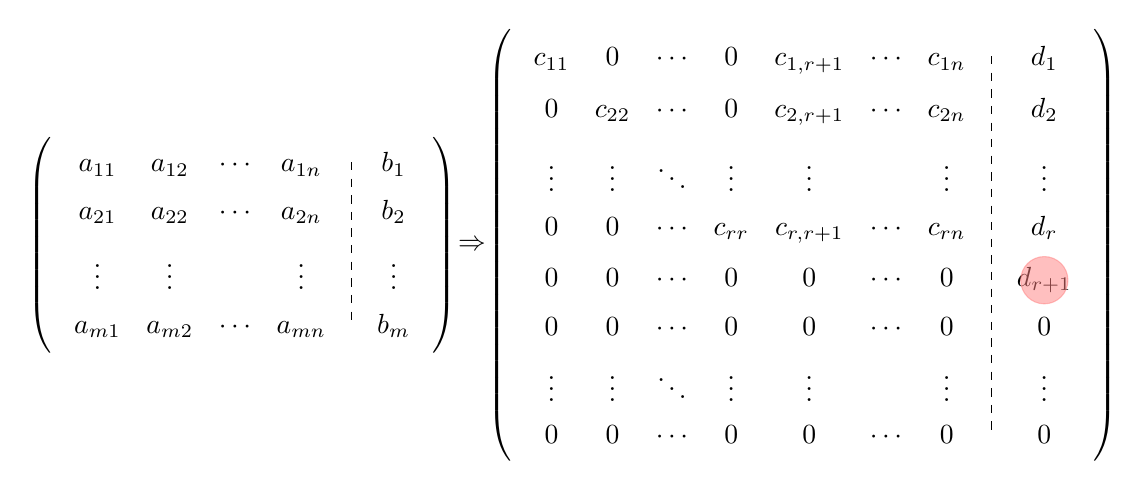
\begin{tikzpicture}
 		\matrix(MM) [matrix of math nodes,nodes in empty cells,
 		column sep=0.6ex,row sep=.5ex,ampersand replacement=\&,left delimiter=(,right delimiter=)] {
 			a_{11} \&  a_{12} \&  \cd \& a_{1n} \& \&  b_1\\
 			a_{21} \&  a_{22} \&  \cd \& a_{2n} \& \&  b_2\\
 			\vd   \&  \vd   \&      \&  \vd  \& \& \vd \\
 			a_{m1} \&  a_{m2} \&  \cd \& a_{mn} \& \&  b_m\\
 		};
 		\draw[dashed] (MM-1-5.north) -- (MM-4-5);
 		\matrix (M2) [right=.05in of MM,matrix of math nodes]  { 
 			\Rightarrow\\
 		};
 		\matrix(MM) [right=.05in of M2,matrix of math nodes,nodes in empty cells,
 		column sep=0.6ex,row sep=.5ex,ampersand replacement=\&,left delimiter=(,right delimiter=)] {
 			c_{11} \&   0 \& \cd \&  0 \& c_{1,r+1} \& \cd \& c_{1n} \& \& d_1\\
 			0   \& c_{22} \& \cd \&  0 \& c_{2,r+1} \& \cd \& c_{2n} \& \& d_2\\
 			\vd \& \vd \& \dd \&\vd \& \vd     \&     \& \vd   \& \& \vd\\
 			0   \&  0  \& \cd \& c_{rr} \& c_{r,r+1} \& \cd \& c_{rn} \& \& d_r\\
 			0   \&  0  \& \cd \& 0 \& 0 \& \cd \& 0 \&  \& d_{r+1}\\
 			0   \&  0  \& \cd \& 0 \& 0 \& \cd \& 0 \&  \& 0\\          
 			\vd \& \vd \& \dd \&\vd \& \vd     \&     \& \vd   \& \& \vd\\
 			0   \&  0  \& \cd \& 0 \& 0 \& \cd \& 0 \&  \& 0\\
 		};
 		\draw[dashed] (MM-1-8.north) -- (MM-8-8);
 		\filldraw[opacity=0.5,red!50] (MM-5-9) circle (0.3cm);
 		\end{tikzpicture}      
 	\end{figure}  
 	其中$c_{ii}=1~(i=1,2,\cd,r)$。
\end{proof}
\end{small}
\end{frame}
 	
\begin{frame}\ft{\secname}
\begin{small}
\begin{proof}[续]
 			
 	因此,对于任何矩阵$\A$,都可经过初等行变换将其化为行简化阶梯形矩阵,即存在初等矩阵$\PP_1,\PP_2,\cd,\PP_s$使得
 	$$
 	\PP_s \cd \PP_2 \PP_1 \A = \mathbf{U}.
 	$$
 	\pause
 	当$\A$为$n$阶可逆矩阵时,行简化阶梯形矩阵也是可逆矩阵,从而$\mathbf{U}$必为单位矩阵$\I$.
 \end{proof}
\end{small}

\end{frame}


\begin{frame}\ft{\secname}
\begin{tuilun}
  可逆矩阵$\A$可以表示为若干个初等矩阵的乘积。
\end{tuilun}
\pause
\begin{proof}
由上述定理,必存在初等矩阵$\PP_1,\PP_2,\cd,\PP_s$使得
$$
\PP_s \cd \PP_2 \PP_1 \A = \I,
$$\pause
于是
$$
\A = (\PP_s \cd \PP_2 \PP_1)^{-1} = \PP_1^{-1}\PP_2^{-1}\cd\PP_s^{-1},
$$
亦即
$$
\A^{-1}=\PP_s \cd \PP_2 \PP_1.
$$
\end{proof}
\end{frame}


\begin{frame}\ft{\secname}
\begin{tuilun}
  如果对可逆矩阵$\A$与同阶单位矩阵$\I$做同样的初等行变换,那么当$\A$变为单位阵时,
  $\I$就变为$\A^{-1}$,即
  $$\textcolor{acolor3}{
    \left(
      \begin{array}{cc}
        \A & \I
      \end{array}
    \right) \xrightarrow[]{\mbox{初等行变换}} \left(
      \begin{array}{cc}
        \I & \A^{-1}
      \end{array}
    \right)
  } 
  $$
  同理,
$$\textcolor{acolor3}{
  \left(
    \begin{array}{c}
      \A\\
      \I
    \end{array}
  \right) \xrightarrow[]{\mbox{初等列变换}} \left(
    \begin{array}{c}
      \I \\
      \A^{-1}
    \end{array}
  \right)
} 
$$
\end{tuilun}
\pause

\begin{zhu}
\textcolor{acolor1}{该推论给出了求可逆矩阵的逆的一种有效方法,请大家熟练掌握。}
\end{zhu}
\end{frame}


\begin{frame}\ft{\secname}
\begin{li}
  求$
  \A=\left(
    \begin{array}{rrr}
      0&2&-1\\
      1&1&2\\
      -1&-1&-1
    \end{array}
  \right)
  $
  的逆矩阵。
\end{li}
\end{frame}


\begin{frame}\ft{\secname}
\begin{jie}

$$
\begin{aligned}
&\left(
  \begin{array}{c|c}
    \A & \I
  \end{array}
\right)=\left(
  \begin{array}{rrr|rrr}
    0 &  2 & -1 &  1 & 0 & 0\\
    1 &  1 &  2 &  0 & 1 & 0\\
    -1 & -1 & -1 &  0 & 0 & 1\\              
  \end{array}
\right) \\ \pause
&\xrightarrow[]{r_1\leftrightarrow r_2}\left(
  \begin{array}{rrr|rrr}
    1 &  1 &  2 &  0 & 1 & 0\\
    0 &  2 & -1 &  1 & 0 & 0\\
    -1 & -1 & -1 &  0 & 0 & 1\\          
  \end{array}
\right) \pause
\xrightarrow[]{r_3+ r_1}\left(
  \begin{array}{rrr|rrr}
    1 &  1 &  2 & 0 & 1 & 0\\
    0 &  2 & -1 & 1 & 0 & 0\\
    0 &  0 &  1 & 0 & 1 & 1\\          
  \end{array}
\right)\\\pause
&\xrightarrow[r_2+r_3]{r_1+ r_3\times(-2)}\left(
  \begin{array}{rrr|rrr}
    1 &  1 &  0  & 0 &-1 &-2\\
    0 &  2 &  0  & 1 & 1 & 1\\
    0 &  0 &  1  & 0 & 1 & 1\\    
  \end{array}
\right)\\\pause
&\xrightarrow[r_2\times \frac12]{r_1+ r_2\times(-\frac12)}\left(
  \begin{array}{rrr|rrr}
    1 &  0 &  0  & -\frac12 &-\frac32 &-\frac52\\[.1in]
    0 &  1 &  0  & \frac12 & \frac12 & \frac12 \\[.1in]
    0 &  0 &  1  & 0 & 1 & 1                   
  \end{array}
\right)    
\end{aligned}
$$
\end{jie}
\end{frame}


\begin{frame}\ft{\secname}
\begin{li}
  已知$\A\B\A^T=2\B\A^T+\I$,求$\B$,其中$
  \A = \left(
    \begin{array}{ccc}
      1&0&0\\
      0&1&2\\
      0&0&1
    \end{array}
  \right)
  $
\end{li}
\end{frame}


\begin{frame}\ft{\secname}
\begin{jie}
$$
\A\B\A^T=2\B\A^T+\I ~~ \Rightarrow ~~ (\A-2\I)\B\A^T=\I 
~~ \Rightarrow ~~ \B\A^T = (\A-2\I)^{-1}
$$
\pause
故
$$
\B = (\A-2\I)^{-1} (\A^T)^{-1}  = [\A^T(\A-2\I)]^{-1} 
=(\A^T\A-2\A^T)^{-1}
$$\pause
而
$$
\A^T\A-2\A^T = \left(
  \begin{array}{rrr}
    -1&0&0\\
    0&-1&2\\
    0&-2&3
  \end{array}
\right)
$$ \pause
可求得
$$
\B = \left(
  \begin{array}{rrr}
    -1&0&0\\
    0&3&-2\\
    0&2&-1
  \end{array}
\right)
$$
\end{jie}
\end{frame}


\begin{frame}\ft{\secname}

\begin{tuilun}
  对于$n$个未知数$n$个方程的线性方程组
  $
  \A\xx=\bb,
  $
  如果增广矩阵
  $$
  \textcolor{acolor3}{(\A,~\bb)~~\overset{r}{\sim}~~(\I,\xx)},
  $$
  则$\A$可逆,且$\xx=\A^{-1}\bb$为惟一解。  
\end{tuilun}
\end{frame}


\begin{frame}\ft{\secname}
\begin{li}
  设
  $$
  \A = \left(
    \begin{array}{rrr}
      2&1&-3\\
      1&2&-3\\
      -1&3&2
    \end{array}
  \right),
  ~~
  \bb_1=\left(
    \begin{array}{r}
      1\\
      2\\
      -2
    \end{array}
  \right),
  ~~
  \bb_2=\left(
    \begin{array}{r}
      -1\\
      0\\
      5
    \end{array}
  \right),
  $$
  求$\A\xx=\bb_1$与$\A\xx=\bb_2$的解。
\end{li}
\end{frame}


\begin{frame}\ft{\secname}
\begin{jie}
  $$
  \begin{aligned}
    & (\A~~\textcolor{acolor3}{\bb_1}~~\textcolor{acolor3}{\bb_2})
    = \left(
      \begin{array}{rrrrr}
        2 & 1 & 3 &\textcolor{acolor3}{ 1} & \textcolor{acolor3}{-1}\\
        1 & 2 &-2 &\textcolor{acolor3}{ 2} & \textcolor{acolor3}{ 0}\\
        -1 & 3 & 2 &\textcolor{acolor3}{-2} & \textcolor{acolor3}{ 5}        
      \end{array}\right) \\ \pause
      & \overset{{r_1\leftrightarrow r_2 \atop r_2-2r_1}\atop  r_3+r_1}{\sim}
                               \left(
                               \begin{array}{rrrrr}
                                 1 & 2 &-2 & \textcolor{acolor3}{ 2} & \textcolor{acolor3}{ 0}\\
                                 0 &-3 & 1 & \textcolor{acolor3}{-3} & \textcolor{acolor3}{-1}\\
                                 0 & 5 & 0 & \textcolor{acolor3}{ 0} & \textcolor{acolor3}{ 5}        
                               \end{array}
                                                        \right) \\ \pause
    & \overset{{r_3\leftrightarrow r_2 \atop r_2\div5}\atop  r_3+3r_2}{\sim}
      \left(
      \begin{array}{rrrrr}
        1 & 2 &-2 &\textcolor{acolor3}{ 2} &  \textcolor{acolor3}{0}\\
        0 & 1 & 0 &\textcolor{acolor3}{ 0} &  \textcolor{acolor3}{1}\\
        0 & 0 & 1 &\textcolor{acolor3}{-3} &  \textcolor{acolor3}{2}        
      \end{array}
                              \right)  \pause \overset{r_1-2r_2+2r_3}{\sim}
                              \left(
                              \begin{array}{rrrrr}
                                1 & 0 & 0 & \textcolor{acolor3}{-4} & \textcolor{acolor3}{2}\\
                                0 & 1 & 0 & \textcolor{acolor3}{0} &  \textcolor{acolor3}{1}\\
                                0 & 0 & 1 & \textcolor{acolor3}{-3} &  \textcolor{acolor3}{2}        
                              \end{array}
                                                       \right) 
  \end{aligned}
  $$
\end{jie}

\end{frame}


\begin{frame}\ft{\secname}

\begin{li}
  求解矩阵方程$\A\XX=\A+\XX$,其中
  $
  \A = \left(
    \begin{array}{ccc}
      2&2&0\\
      2&1&3\\
      0&1&0
    \end{array}
  \right)
  $
\end{li}
\end{frame}


\begin{frame}\ft{\secname}
\begin{jie}
原方程等价于
$$
(\A-\I)\XX=\A
$$
\pause
而
$$
\begin{aligned}
&  (\A-\I ~~\textcolor{acolor3}{\A}) =\left(
                       \begin{array}{rrrrrr}
                         1&2& 0&\textcolor{acolor3}{2}&\textcolor{acolor3}{2}&\textcolor{acolor3}{0}\\
                         2&0& 3&\textcolor{acolor3}{2}&\textcolor{acolor3}{1}&\textcolor{acolor3}{3}\\
                         0&1&-1&\textcolor{acolor3}{0}&\textcolor{acolor3}{1}&\textcolor{acolor3}{0}
                       \end{array}
                                                 \right)\\\pause
                                                 &\overset{r_2-2r_1\atop r_2\leftrightarrow r_3}{\sim}
                                                 \left(
                                                 \begin{array}{rrrrrr}
                                                   1& 2& 0&\textcolor{acolor3}{ 2}&\textcolor{acolor3}{ 2}&\textcolor{acolor3}{0}\\
                                                   0& 1&-1&\textcolor{acolor3}{ 0}&\textcolor{acolor3}{ 1}&\textcolor{acolor3}{0}\\
                                                   0&-4& 3&\textcolor{acolor3}{-2}&\textcolor{acolor3}{-3}&\textcolor{acolor3}{3}
                                                 \end{array}
                                                                              \right)     \pause
                       \overset{r_3+4r_2\atop r_3\div(-1)}{\sim}
                       \left(
                       \begin{array}{rrrrrr}
                         1&2& 0&\textcolor{acolor3}{2}&\textcolor{acolor3}{ 2}&\textcolor{acolor3}{ 0}\\
                         0&1&-1&\textcolor{acolor3}{0}&\textcolor{acolor3}{ 1}&\textcolor{acolor3}{ 0}\\
                         0&0& 1&\textcolor{acolor3}{2}&\textcolor{acolor3}{-1}&\textcolor{acolor3}{-3}
                       \end{array}
                                                  \right) \\ \pause
                     &  
                       \overset{r_3+4r_2\atop r_3\div(-1)}{\sim}
                       \left(
                       \begin{array}{rrrrrr}
                         1&0&0&\textcolor{acolor3}{-2}&\textcolor{acolor3}{2}&\textcolor{acolor3}{6}\\
                         0&1&0&\textcolor{acolor3}{2}&\textcolor{acolor3}{0}&\textcolor{acolor3}{-3}\\
                         0&0&1&\textcolor{acolor3}{2}&\textcolor{acolor3}{-1}&\textcolor{acolor3}{-3}
                       \end{array}
                                                 \right)
\end{aligned}
$$
\end{jie}
\end{frame}


\begin{frame}\ft{\secname}
\begin{li}
  当$a,b$满足什么条件时,矩阵$\A=\left(
    \begin{array}{rrrr}
      0&1&2&3\\
      1&4&7&10\\
      -1&0&1&b\\
      a&2&3&4
    \end{array}
  \right)$
  不可逆。
\end{li}
\end{frame}


\begin{frame}\ft{\secname}
\begin{jie}
$$
\begin{aligned}
  \left(
  \begin{array}{rrrr}
  0&1&2&3\\
  1&4&7&10\\
  -1&0&1&b\\
  a&2&3&4
  \end{array}
  \right)\pause\xrightarrow[c_2\leftrightarrow c_3]{c_1\leftrightarrow c_2} &
  \left(
    \begin{array}{rrrr}
      1 & 2 & 0 & 3\\
      4 & 7 & 1 & 10\\
      0 & 1 & -1 & b\\
      2 & 3 & a & 4\\
    \end{array}
  \right)\\\pause
  \xrightarrow[r_4+r_1\times(-2)]{r_2+r_1\times(-4)}&
  \left(
    \begin{array}{rrrr}
      1 & 2 & 0 & 3\\
      0 & -1 & 1 & -2\\
      0 & 1 & -1 & b\\
      0 & -1 & a & -2\\
    \end{array}
  \right)\\\pause
  \xrightarrow[r_4+r_2\times(-1)]{r_3+r_2}&
  \left(
    \begin{array}{rrrr}      
      1 & 2 & 0 & 3\\
      0 & -1 & 1 & -2\\
      0 & 0 & -1 & b\\
      0 & 0 & a-1 & 0\\
    \end{array}
  \right)
\end{aligned}
$$\pause
由此可知$\A$不可逆的条件是$(a-1)b=0$。
\end{jie}
\end{frame}


  \section{矩阵分块}
\begin{frame}\ft{\secname}

矩阵
\begin{figure}[htbp]
  \centering
  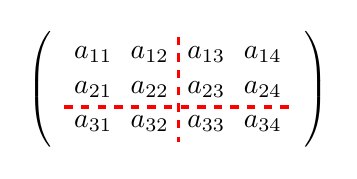
\begin{tikzpicture}
    \matrix(A) [matrix of math nodes,nodes in empty cells,ampersand replacement=\&,left delimiter=(,right delimiter=)] {
      a_{11} \& a_{12} \& a_{13}  \& a_{14} \\
      a_{21} \& a_{22} \& a_{23}  \& a_{24} \\
      a_{31} \& a_{32} \& a_{33}  \& a_{34} \\
    };
    \draw[red, dashed, very thick] (A-1-2.north east) -- (A-3-2.south east) (A-2-1.south west) -- (A-2-4.south east);;
  \end{tikzpicture}
\end{figure}
可记为
$$
\left(
  \begin{array}{cc}
    \A_{11} &  \A_{12}\\
    \A_{21} &  \A_{22}
  \end{array}
\right)
$$
其中
$$
\begin{array}{ll}
  \A_{11} = 
  \left(
  \begin{array}{cc}
    a_{11} &  a_{12}\\
    a_{21} &  a_{22}
  \end{array} \right),
           &
             \A_{12} = 
             \left(
             \begin{array}{cc}
               a_{13} &  a_{14}\\
               a_{23} &  a_{24}
             \end{array}
                        \right)\\ [0.3cm]
  \A_{21} = 
  \left(
  \begin{array}{cc}
    a_{31} &  a_{32}
  \end{array}\right) ,
           &
             \A_{22} = 
             \left(
             \begin{array}{cc}
               a_{33} &  a_{34}
             \end{array}
                        \right)    
\end{array}
$$
\end{frame}

\begin{frame}\ft{\secname}
\begin{dingyi}[矩阵的按行分块]
  $$
  \A = \left(
    \begin{array}{cccc}
      a_{11} & a_{12} & \cd & a_{1n}\\
      a_{21} & a_{22} & \cd & a_{2n}\\
      \vd & \vd & & \vd \\
      a_{m1} & a_{m2} & \cd & a_{mn}
    \end{array}
  \right)
  = \left(
    \begin{array}{c}
      \abd_1\\
      \abd_2\\
      \vd \\
      \abd_m
    \end{array}
  \right)
  $$
  其中
  $$
  \abd_i = (a_{i1}, ~a_{i2}, ~\cd, ~a_{in})
  $$
\end{dingyi}
\end{frame}

\begin{frame}\ft{\secname}
\begin{dingyi}[矩阵的按列分块]
  $$
  \B = \left(
    \begin{array}{cccc}
      b_{11} & b_{12} & \cd & b_{1s}\\
      b_{21} & b_{22} & \cd & b_{2s}\\
      \vd & \vd & & \vd \\
      b_{n1} & b_{n2} & \cd & b_{ns}
    \end{array}
  \right)
  = \left(
    \begin{array}{c}
      \bb_1, ~ \bb_2, ~ \cd, \bb_s
    \end{array}
  \right)
  $$
  其中
  $$
  \bb_j = \left(
    \begin{array}{c}
      b_{1j}\\
      b_{2j}\\
      \vd\\
      b_{nj}
    \end{array}
  \right)
  $$
\end{dingyi}
\end{frame}

\begin{frame}\ft{\secname}
当$n$阶矩阵$\A$中非零元素都集中在主对角线附近,有时可分块成如下\textcolor{acolor3}{对角块矩阵}
$$
\A = \left(
  \begin{array}{cccc}
    \A_1 & & &\\
    &\A_2&&\\
    &&\dd&\\
    &&&\A_m
  \end{array}
\right)
$$
其中$\A_i$为$r_i$阶方阵($i=1,2,\cd,m$),且
$$
\sum_{i=1}^m r_i = n.
$$

\end{frame}

\begin{frame}\ft{\secname}
如
\begin{figure}
  \centering
  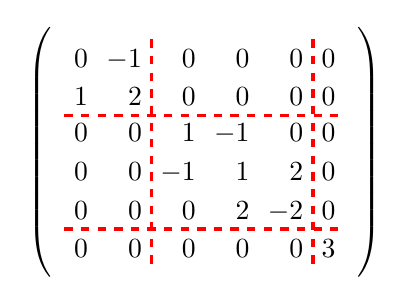
\begin{tikzpicture}       
    [column 1/.style={anchor=base east},
    column 2/.style={anchor=base east},
    column 3/.style={anchor=base east},
    column 4/.style={anchor=base east},
    column 5/.style={anchor=base east},
    column 6/.style={anchor=base east}]
    \matrix(A) [matrix of math nodes,nodes in empty cells,ampersand replacement=\&,left delimiter=(,right delimiter=)] {
    0 \& -1 \& 0 \& 0 \& 0 \& 0\\
    1 \&  2 \& 0 \& 0 \& 0 \& 0\\
    0 \&  0 \& 1 \&-1 \& 0 \& 0\\
    0 \&  0 \&-1 \& 1 \& 2 \& 0\\
    0 \&  0 \& 0 \& 2 \&-2 \& 0\\
    0 \&  0 \& 0 \& 0 \& 0 \& 3\\
  };
    \draw[red, dashed, very thick] 
    (A-1-2.north east) -- (A-6-2.south east)
    (A-1-5.north east) -- (A-6-5.south east) 
    (A-2-1.south west) -- (A-2-6.south east)
    (A-5-1.south west) -- (A-5-6.south east);

  \end{tikzpicture}
\end{figure}

\end{frame}

\begin{frame}\ft{\secname}



\begin{dingyi}[分块矩阵的加法]
  设$\A, \B$为同型矩阵,采用相同的分块法,有
  $$
  \A = \left(
    \begin{array}{ccc}
      \A_{11} & \cd & \A_{1r} \\
      \vd   &     & \vd   \\
      \A_{s1} & \cd & \A_{sr}
    \end{array}
  \right), \ \ 
  \B = \left(
    \begin{array}{ccc}
      \B_{11} & \cd & \B_{1r} \\
      \vd   &     & \vd   \\
      \B_{s1} & \cd & \B_{sr}
    \end{array}
  \right),
  $$
  其中$\A_{ij}$与$\B_{ij}$为同型矩阵,则
  $$
  A = \left(
    \begin{array}{ccc}
      \A_{11} + \B_{11}  & \cd & \A_{1r} + \B_{1r} \\
      \vd   &     & \vd   \\
      \A_{s1} + \B_{s1}  & \cd & \A_{sr} + \B_{sr}
    \end{array}
  \right).
  $$
\end{dingyi}
\end{frame}

\begin{frame}\ft{\secname}

\begin{dingyi}[分块矩阵的数乘]
  $$
  \lambda \A = \left(
    \begin{array}{ccc}
      \lambda \A_{11} & \cd & \lambda \A_{1r} \\
      \vd   &     & \vd   \\
      \lambda \A_{s1} & \cd & \lambda \A_{sr}
    \end{array}
  \right)
  $$    
\end{dingyi}
\end{frame}

\begin{frame}\ft{\secname}

\begin{dingyi}[分块矩阵的乘法]
  设$\A$为$m\times n$矩阵, $\B$为$n \times s$矩阵,
  $$
  \A = \left(
    \begin{array}{ccc}
      \A_{11} & \cd & \A_{1s} \\
      \vd   &     & \vd   \\
      \A_{r1} & \cd & \A_{rs}
    \end{array}
  \right), \ \ 
  \B = \left(
    \begin{array}{ccc}
      \B_{11} & \cd & \B_{1t} \\
      \vd   &     & \vd   \\
      \B_{s1} & \cd & \B_{st}
    \end{array}
  \right),
  $$
  其中\textcolor{acolor3}{$\A_{i1}, \A_{i2}, \cd, A_{is}$的列数分别等于$\B_{1j}, \B_{2j}, \cd, \B_{sj}$的行数},则
  $$
  \A \B = \left(
    \begin{array}{ccc}
      \C_{11}   & \cd & \C_{1t}  \\
      \vd   &     & \vd   \\
      \C_{r1}   & \cd & \C_{rt}
    \end{array}
  \right),
  $$
  其中
  $$
  \C_{ij} = \sum_{k=1}^s \A_{ik} \B_{kj}.
  $$
\end{dingyi}
\end{frame}

\begin{frame}\ft{\secname}


\begin{li} 
  用分块矩阵的乘法计算$\A\B$,其中
  $$
  \A = \left(
    \begin{array}{rrrrr}
      1&0&0&0&0\\
      0&1&0&0&0\\
      -1&2&1&0&0\\
      1&1&0&1&0\\
      -2&0&0&0&1
    \end{array}
  \right), \quad
  \B = \left(
    \begin{array}{rrrrr}
      3&2&0&1&0\\
      1&3&0&0&1\\
      -1&0&0&0&0\\
      0&-1&0&0&0\\
      0&0&-1&0&0
    \end{array}
  \right)
  $$
\end{li}
\end{frame}

\begin{frame}\ft{\secname}
\begin{center}
  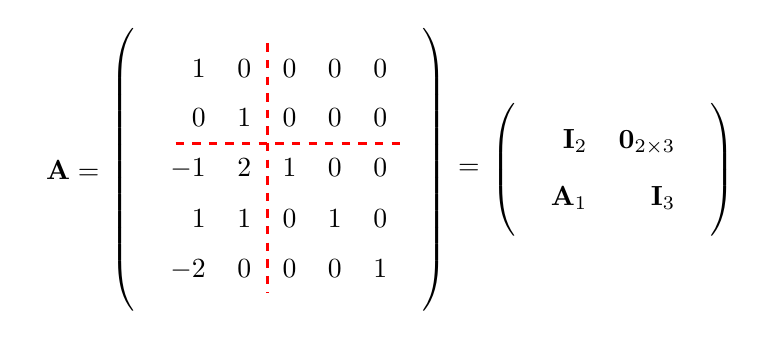
\begin{tikzpicture}       
    [column 1/.style={anchor=base east},
    column 2/.style={anchor=base east},
    column 3/.style={anchor=base east},
    column 4/.style={anchor=base east},
    column 5/.style={anchor=base east}]
    \matrix(A1) [matrix of math nodes]{
    \A = \\
  };
  \matrix(A2) [right=.1in of A1,matrix of math nodes,nodes in empty cells,inner sep=0.2cm,ampersand replacement=\&,left delimiter=(,right delimiter=)] {
    1 \& 0 \& 0 \& 0 \& 0 \\
    0 \& 1 \& 0 \& 0 \& 0 \\
    -1 \& 2 \& 1 \& 0 \& 0 \\
    1 \& 1 \& 0 \& 1 \& 0 \\
    -2 \& 0 \& 0 \& 0 \& 1 \\
  };
    \draw[red, dashed, very thick] 
    (A2-1-2.north east) -- (A2-5-2.south east)
    (A2-2-1.south west) -- (A2-2-5.south east);
    \matrix(A3) [right=.1in of A2,matrix of math nodes]{
    = \\
  };
    \matrix(A4) [right=.1in of A3,matrix of math nodes,nodes in empty cells,inner sep=0.2cm,ampersand replacement=\&,left delimiter=(,right delimiter=)] {
    \II_2 \& \zero_{2\times 3} \\
    \A_1 \& \II_3\\
  };
  \end{tikzpicture}
\end{center}


\begin{center}
  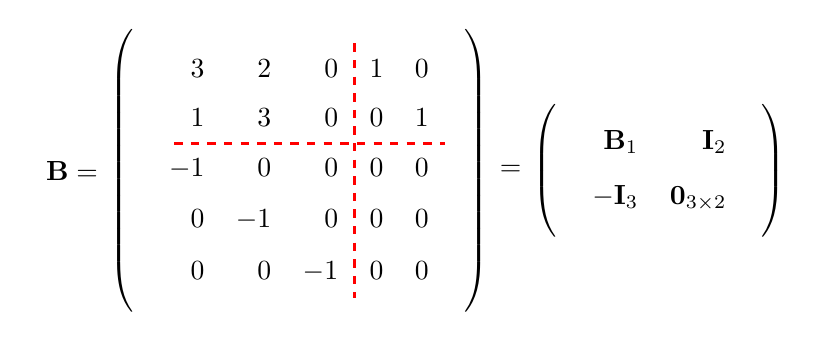
\begin{tikzpicture}       
    [column 1/.style={anchor=base east},
    column 2/.style={anchor=base east},
    column 3/.style={anchor=base east},
    column 4/.style={anchor=base east},
    column 5/.style={anchor=base east}]
    \matrix(A1) [matrix of math nodes]{
    \B = \\
  };
    \matrix(A2) [right=.1in of A1,matrix of math nodes,nodes in empty cells,inner sep=0.2cm,ampersand replacement=\&,left delimiter=(,right delimiter=)] {
    3\&2\&0\&1\&0\\
    1\&3\&0\&0\&1\\
    -1\&0\&0\&0\&0\\
    0\&-1\&0\&0\&0\\
    0\&0\&-1\&0\&0\\
  };
    \draw[red, dashed, very thick] 
    (A2-1-3.north east) -- (A2-5-3.south east)
    (A2-2-1.south west) -- (A2-2-5.south east);
    \matrix(A3) [right=.1in of A2,matrix of math nodes]{
    = \\
  };
    \matrix(A4) [right=.1in of A3,matrix of math nodes,nodes in empty cells,inner sep=0.2cm,ampersand replacement=\&,left delimiter=(,right delimiter=)] {
    \B_1 \& \II_2 \\
    -\II_3 \& \zero_{3\times 2}\\
  };
  \end{tikzpicture}
\end{center}
\end{frame}

\begin{frame}\ft{\secname}
则
$$
\A\B = \left(
  \begin{array}{cc}
    \II_2 & \zero\\
    \A_1 & \II_3
  \end{array}
\right)\left(
  \begin{array}{cc}
    \B_1 & \II_2\\
    -\II_3 & \zero
  \end{array}
\right) = \left(
  \begin{array}{cc}
    \B_1 & \II_2\\
    \A_1\B_1-\II_3 & \A_1
  \end{array}
\right)
$$
其中
$$
\A_1\B_1-\II_3 = \left(
  \begin{array}{rr}
    -1&2\\
    1&1\\
    -2&0
  \end{array}
\right)\left(
  \begin{array}{rrr}
    3&2&0\\
    1&3&0
  \end{array}
\right)-\left(
  \begin{array}{ccc}
    1&0&0\\
    0&1&0\\
    0&0&1
  \end{array}
\right)=\left(
  \begin{array}{rrr}
    -2&4&0\\
    4&4&0\\
    -6&-4&-1
  \end{array}
\right)
$$
\end{frame}

\begin{frame}\ft{\secname}

\begin{li}
  设$\A$为$m\times n$矩阵,$\B$为$n\times s$矩阵,$\B$按列分块成$1\times s$分块矩阵,
  将$\A$看成$1\times 1$分块矩阵,则
  $$
  \A\B=\A(\bb_1,\bb_2,\cd,\bb_s)=(\A\bb_1,\A\bb_2,\cd,\A\bb_s)      
  $$
  若已知$\A\B=0$,则显然
  $$
  \A\bb_j=0, \quad j=1,2,\cd,s.
  $$
  因此,$\B$的每一列$\bb_j$都是线性方程组$\A\xx=0$的解。
\end{li}    
\end{frame}

\begin{frame}\ft{\secname}
\begin{li}
  设$\A^T\A=\zero$,证明$\A=\zero$.
\end{li}
\pause
\begin{proof}
设$\A=(a_{ij})_{m\times n}$,把$\A$用列向量表示为$\A=(\abd_1, ~\abd_2,~\cd,~\abd_n)$,则
$$
\A^T\A = \left(
  \begin{array}{c}
    \abd_1^T\\
    \abd_2^T\\
    \cd \\
    \abd_n^T
  \end{array}
\right) (\abd_1, ~\abd_2,~\cd,~\abd_n) = \left(
  \begin{array}{cccc}
    \abd_1^T\abd_1 & \abd_1^T\abd_2 & \cd & \abd_1^T\abd_n\\
    \abd_2^T\abd_1 & \abd_2^T\abd_2 & \cd & \abd_2^T\abd_n\\
    \vd & \vd & & \vd \\
    \abd_n^T\abd_1 & \abd_n^T\abd_2 & \cd & \abd_n^T\abd_n
  \end{array}
\right)
$$
\pause
因为$\A^T\A=\zero$,故
$$
\abd_i^T \abd_j = 0, \quad i,j=1,2,\cd,n.
$$
\pause
特别地,有
$$
\abd_j^T \abd_j = 0, \quad j=1,2,\cd,n,
$$
即
$$
a_{1j}^2+a_{2j}^2+\cd+a_{mj}^2=0  ~\Rightarrow~ a_{1j}=a_{2j}=\cd=a_{mj}=0 ~\Rightarrow~ \A = \zero.
$$
\end{proof}
\end{frame}

\begin{frame}\ft{\secname}

\begin{li}
  若$n$阶矩阵$\C,\D$可以分块成同型对角块矩阵,即
  $$
  \C = \left(
    \begin{array}{cccc}
      \C_1&&&\\
      &\C_2&&\\
      &&\cd&\\
      &&&\C_m
    \end{array}
  \right),\quad
  \D = \left(
    \begin{array}{cccc}
      \D_1&&&\\
      &\D_2&&\\
      &&\cd&\\
      &&&\D_m
    \end{array}
  \right)
  $$
  其中$\C_i$和$\D_i$为同阶方阵($i=1,2,\cd,m$),则
  $$
  \C\D = \left(
    \begin{array}{cccc}
      \C_1\D_1&&&\\
      &\C_2\D_2&&\\
      &&\cd&\\
      &&&\C_m\D_m
    \end{array}
  \right)
  $$
\end{li}

\end{frame}

\begin{frame}\ft{\secname}





\begin{li}
  证明:若方阵$\A$为可逆的上三角阵,则$\A^{-1}$也为上三角阵。
\end{li}
\end{frame}

\begin{frame}\ft{\secname}
\begin{proof}
对阶数$n$用数学归纳法。\pause
\begin{itemize}
\item[1] 当$n=1$时,$(a)^{-1}=(\frac1a)$,结论成立。 \pause
\item[2] 假设命题对$n-1$阶可逆上三角矩阵成立,考虑$n$阶情况,设
  \begin{center}
    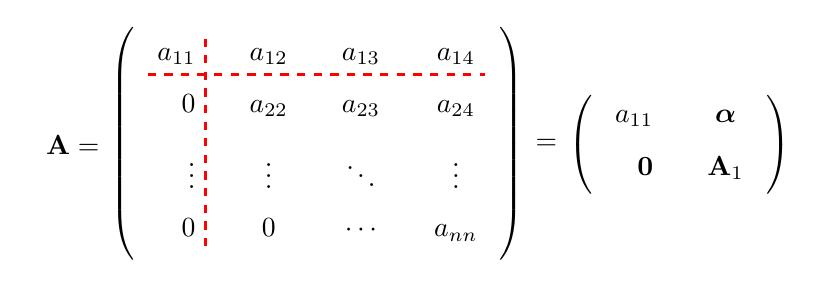
\begin{tikzpicture} [column 1/.style={anchor=base east}]
      \matrix (M) [matrix of math nodes]  { 
      \A = \\
    };
      \matrix(MM) [right=.1in of M, matrix of math nodes,nodes in empty cells,
      column sep=3ex,row sep=1ex,ampersand replacement=\&,left delimiter=(,right delimiter=)] {
      a_{11} \& a_{12} \& a_{13}  \& a_{14} \\
      0    \& a_{22} \& a_{23}  \& a_{24} \\
      \vd  \& \vd   \& \dd  \& \vd \\
      0    \& 0     \& \cd  \& a_{nn} \\
    };

      \draw[red, dashed, very thick]
      (MM-1-1.north east) -- (MM-4-1.south east)
      (MM-1-1.south west) -- (MM-1-4.south east);

      \matrix (MMM) [right=.1in of MM,matrix of math nodes]  { 
      = \\
    };
      \matrix(MMMM) [right=.1in of MMM, matrix of math nodes,nodes in empty cells,
      column sep=3ex,row sep=1ex,ampersand replacement=\&,left delimiter=(,right delimiter=)] {
      a_{11} \& \alphabd\\
      \zero \& \A_1\\
    };
    \end{tikzpicture}        
  \end{center}
  其中$\A_1$为$n-1$阶可逆上三角阵。
\end{itemize}
\end{proof}
\end{frame}

\begin{frame}\ft{\secname}
\begin{proof}[续]
设$\A$的逆阵为
$$
\begin{aligned}
\B = \left(
  \begin{array}{cc}
    b_{11} & \betabd\\
    \gammabd & \B_1 
  \end{array}    
\right),  
\end{aligned}
$$
其中
$$
\begin{aligned}
 \betabd = \left(
  \begin{array}{c}
    b_{12}\\
    \vd \\
    b_{1n}
  \end{array}
\right)^T,  
\quad \gammabd = \left(
  \begin{array}{c}
    b_{21}\\
    \vd \\
    b_{n1}
  \end{array}
\right), \quad
\B_1 = \left(
  \begin{array}{ccc}
    b_{22} & \cd & b_{2n}\\
    \vd   & \dd & \vd \\
    b_{n2} & \cd & b_{nn}
  \end{array}
\right),
\end{aligned}
$$\pause
则
$$
\begin{aligned}
\A\B &= \left(
  \begin{array}{cc}
    a_{11} & \alphabd \\
    \zero & \A_1
  \end{array}
\right)\left(
  \begin{array}{cc}
    b_{11} & \betabd \\
    \gammabd & \B_1
  \end{array}
\right) \\
& = \left(
  \begin{array}{cc}
    a_{11}b_{11}+\alphabd\gammabd & a_{11}\betabd+\alphabd \B_1\\
    \A_1\gammabd & \A_1\B_1
  \end{array}
\right)  \textcolor{acolor3}{
= \left(
  \begin{array}{cc}
    1 & \zero \\
    \zero & \II_{n-1}
  \end{array}
\right)
}
\end{aligned}
  $$
\end{proof}
\end{frame}

\begin{frame}\ft{\secname}
\begin{proof}[续]
          于是
  $$
  \begin{array}{l}
    \A_1 \gammabd = \zero ~ \Rightarrow ~ \gammabd=\zero, \\[0.2cm]
    \A_1\B_1 = \II_1 ~\Rightarrow~ \B_1=\A_1^{-1}.
  \end{array}
  $$\pause
  由归纳假设,$\B_1$为$n-1$阶上三角矩阵,因此
  $$
  \A^{-1} = \B = \left(
    \begin{array}{cc}
      b_{11} & \betabd\\
      \zero & \B_1 
    \end{array}    
  \right)
  $$
  为上三角矩阵。
\end{proof}
\end{frame}

\begin{frame}\ft{\secname}



\begin{dingyi}[分块矩阵的转置]
  分块矩阵$\A=(\A_{kl})_{s\times t}$的转置矩阵为
  $$
  \A^T = (\B_{lk})_{t\times s},
  $$
  其中$\B_{lk}=\A_{kl}$.
\end{dingyi}
\pause
\begin{li}
  $$
  \A = \left(
    \begin{array}{ccc}
      \A_{11} & \A_{12} & \A_{13}\\
      \A_{21} & \A_{22} & \A_{23}
    \end{array}
  \right) ~\Rightarrow~
  \A = \left(
    \begin{array}{cc}
      \A_{11}^T & \A_{21}^T \\[0.2cm]
      \A_{12}^T & \A_{22}^T \\[0.2cm]
      \A_{13}^T & \A_{23}^T
    \end{array}
  \right)
  $$
\pause
  $$
  \B \xlongequal[]{\mbox{按行分块}} \left(
    \begin{array}{c}
      \bb_1\\
      \bb_2\\
      \vd\\
      \bb_m
    \end{array}
  \right) ~\Rightarrow~
  \B^T = \left(
    \begin{array}{cccc}
      \bb_1^T & \bb_2^T & \cd & \bb_m^T
    \end{array}
  \right)
  $$
\end{li}



\end{frame}

\begin{frame}\ft{\secname}


\begin{dingyi}[可逆分块矩阵的逆矩阵]
  对角块矩阵(准对角矩阵)
  $$
  \A = \left(
    \begin{array}{cccc}
      \A_1&&&\\
          &\A_2&&\\
          &&\dd&\\
          &&&\A_m
    \end{array}
  \right)
  $$
  的行列式为$|\A|=|\A_1||\A_2|\cd|\A_m|$,因此,$\A$可逆的充分必要条件为
  $$
  |\A_i|\ne 0, \quad i=1,2,\cd, m.
  $$

  其逆矩阵为
  $$
  \A^{-1} = \left(
    \begin{array}{cccc}
      \A_1^{-1}&&&\\
               &\A_2^{-1}&&\\
               &&\dd&\\
               &&&\A_m^{-1}
    \end{array}
  \right)
  $$
\end{dingyi}
\end{frame}

\begin{frame}\ft{\secname}
分块矩阵的作用:
\begin{itemize}
\item   用分块矩阵求逆矩阵,可将高阶矩阵的求逆转化为低阶矩阵的求逆。
\item   一个$2\times 2$的分块矩阵求逆,可以根据逆矩阵的定义,用解矩阵方程的方法解得。
\end{itemize}
\end{frame}

\begin{frame}\ft{\secname}
\begin{li}
  设$\A=\left(
    \begin{array}{cc}
      \B&\zero\\
      \C&\D
    \end{array}
  \right)$,其中$\B,\D$皆为可逆矩阵,证明$\A$可逆并求$\A^{-1}$.
\end{li}
\end{frame}

\begin{frame}\ft{\secname}
\begin{jie}
  因$|\A|=|\B||\D|\ne 0$,故$\A$可逆。\pause 设$\A^{-1}=\left(
    \begin{array}{cc}
      \X&\Y\\
      \Z&\T
    \end{array}
  \right)$,则
  $$
  \left(
    \begin{array}{cc}
      \B&\zero\\
      \C&\D
    \end{array}
  \right) \left(
    \begin{array}{cc}
      \X&\Y\\
      \Z&\T
    \end{array}
  \right)=\left(
    \begin{array}{cc}
      \B\X&\B\Y\\
      \C\X+\D\Z&\C\Y+\D\T
    \end{array}
  \right) = \left(
    \begin{array}{cc}
      \II & \zero\\
      \zero & \II
    \end{array}
  \right)
  $$
\pause
  由此可知
  $$
  \begin{array}{ll}
    \B\X = \II   & \Rightarrow ~ \X = \B^{-1}\\[0.2cm]
    \B\Y = \zero & \Rightarrow ~ \Y = \zero\\[0.2cm]
    \C\X+\D\Z = \zero & \Rightarrow ~ \Z = -\D^{-1}\C\B^{-1}\\[0.2cm]
    \C\Y+\D\T = \II & \Rightarrow ~ \T = \D^{-1}
  \end{array}
  $$
\pause
  故
  $$
  \A^{-1} = \left(
    \begin{array}{cc}
      \B^{-1} & \zero\\
      -\D^{-1}\C\B^{-1} & \D^{-1}
    \end{array}
  \right).
  $$
\end{jie}
\end{frame}

\begin{frame}\ft{\secname}




\begin{dingyi}[分块矩阵的初等变换与分块初等矩阵]
  对于分块矩阵
  $$
  \A = \left(
    \begin{array}{cc}
      \A_{11} & \A_{12}\\
      \A_{21} & \A_{22}
    \end{array}
  \right)
  $$
  同样可以定义它的3类初等行变换与列变换,并相应地定义3类分块矩阵:
  \begin{itemize}
  \item[(i)] 分块倍乘矩阵($\C_1,\C_2$为可逆阵)
    $$
    \left(
      \begin{array}{cc}
        \C_1 & \zero\\
        \zero & \II_n
      \end{array}
    \right) ~~\mbox{或}~~
    \left(
      \begin{array}{cc}
        \II_m & \zero\\
        \zero & \C_2
      \end{array}
    \right)
    $$
  \item[(ii)] 分块倍加矩阵
    $$
    \left(
      \begin{array}{cc}
        \II_m & \zero\\
        \C_3 & \II_n
      \end{array}
    \right) ~~\mbox{或}~~
    \left(
      \begin{array}{cc}
        \II_m & \C_4\\
        \zero & \II_n
      \end{array}
    \right)
    $$
  \item[(iii)] 分块对换矩阵
    $$
    \left(
      \begin{array}{cc}
        \zero & \II_n\\
        \II_m & \zero
      \end{array}
    \right)
    $$
  \end{itemize}
\end{dingyi}
\end{frame}

\begin{frame}\ft{\secname}

\begin{li}
  设$n$阶矩阵$\A$分块表示为
  $$
  \A = \left(
    \begin{array}{cc}
      \A_{11} & \A_{12}\\
      \A_{21} & \A_{22}
    \end{array}
  \right)
  $$
  其中$\A_{11},\A_{22}$为方阵,且$\A$与$\A_{11}$可逆。证明:$\A_{22}-\A_{21}\A_{11}^{-1}\A_{12}$可逆,并求$\A^{-1}$。
\end{li}
\end{frame}

\begin{frame}\ft{\secname}
\begin{jie}
  构造分块倍加矩阵
  $$
  \PP_1 = \left(
    \begin{array}{cc}
      \II_1 & \zero\\
      -\A_{21}\A_{11}^{-1} & \II_2
    \end{array}
  \right)
  $$
  则$$
  \PP_1\A = \left(
    \begin{array}{cc}
      \A_{11} & \A_{12} \\
      \zero & \A_{22}-\A_{21}\A_{11}^{-1}\A_{12}
    \end{array}
  \right)
  $$
  两边同时取行列式可知
  $$
  |\A| = |\PP_1\A| = |\A_{11}|\cdot |\A_{22}-\A_{21}\A_{11}^{-1}\A_{12}|
  $$
  故$\A_{22}-\A_{21}\A_{11}^{-1}\A_{12}$可逆。
\end{jie}
\end{frame}

\begin{frame}\ft{\secname}
\begin{jie}[续]
  $$
  \PP_1\A = \left(
    \begin{array}{cc}
      \A_{11} & \A_{12} \\
      \zero & \A_{22}-\A_{21}\A_{11}^{-1}\A_{12}
    \end{array}
  \right)\xlongequal[]{\textcolor{acolor3}{\ds \QQ=\A_{22}-\A_{21}\A_{11}^{-1}\A_{12}}}
  \left(
    \begin{array}{cc}
      \A_{11} & \A_{12} \\
      \zero & \QQ
    \end{array}
  \right)
  $$ \pause
  构造分块倍加矩阵
  $$
  \PP_2 = \left(
    \begin{array}{cc}
      \II_1 & -\A_{12}\QQ^{-1}\\
      \zero & \II_2
    \end{array}
  \right)
  $$ \pause
  则
  $$
  \PP_2\PP_1\A = \left(
    \begin{array}{cc}
      \A_{11} & \zero\\
      \zero & \QQ
    \end{array}
  \right)
  $$ \pause
  于是
  $$
  \begin{array}{rl}
    \A^{-1} & = \left(
      \begin{array}{cc}
        \A_{11}^{-1} & \zero\\
        \zero & \QQ^{-1}
      \end{array}
    \right)\left(
      \begin{array}{cc}
        \II_1 & -\A_{12}\QQ^{-1}\\
        \zero & \II_2
      \end{array}
    \right)\left(
      \begin{array}{cc}
        \II_1 & \zero\\[0.2cm]
        -\A_{21}\A_{11}^{-1} & \II_2
      \end{array}
    \right) \\[0.3in]
    & = \left(
      \begin{array}{cc}
        \A_{11}^{-1} & \zero\\[0.2cm]
        \zero & \QQ^{-1}
      \end{array}
    \right)\left(
      \begin{array}{cc}
        \II_1+ \A_{12}\QQ^{-1}\A_{21}\A_{11}^{-1}& -\A_{12}\QQ^{-1}\\[0.2cm]
        -\A_{21}\A_{11}^{-1} & \II_2
      \end{array}
    \right)\\[0.3in]
    & = \left(
      \begin{array}{cc}
        \A_{11}^{-1}+ \A_{11}^{-1}\A_{12}\QQ^{-1}\A_{21}\A_{11}^{-1}& -\A_{11}^{-1}\A_{12}\QQ^{-1}\\[0.2cm]
        -\QQ^{-1}\A_{21}\A_{11}^{-1} & \QQ^{-1}
      \end{array}
    \right)
  \end{array}
  $$
\end{jie}
\end{frame}

\begin{frame}\ft{\secname}

  \begin{li}
    设$\QQ=\left(
      \begin{array}{cc}
        \A&\B\\
        \C&\D
      \end{array}
    \right)$,且$\A$可逆,证明:
    $$
    |\QQ| = |\A| \cdot |\D-\C\A^{-1}\B|
    $$
  \end{li}\pause
\begin{proof}
  构造分块倍加矩阵
  $$
  \PP_1 = \left(
    \begin{array}{cc}
      \II_1 & \zero\\
      -\C\A^{-1} & \II_2
    \end{array}
  \right)
  $$ \pause
  则
  $$
  \PP_1 \QQ = \left(
    \begin{array}{cc}
      \A & \B\\
      \zero & \D-\C\A^{-1}\B
    \end{array}
  \right)
  $$
\pause
  两边同时取行列式得
  $$
  |\QQ| = |\PP_1\QQ| = |\A|\cdot |\D-\C\A^{-1}\B|.
  $$
\end{proof}
\end{frame}

\begin{frame}\ft{\secname}
  \begin{li}
    设$\A$与$\B$均为$n$阶分块矩阵,证明
    $$
    \left|
      \begin{array}{cc}
        \A&\B\\
        \B&\A
      \end{array}
    \right| = |\A+\B|~|\A-\B|
    $$
  \end{li}
\end{frame}

\begin{frame}\ft{\secname}
\begin{proof}

  将分块矩阵$
  \PP = 
  \left(
    \begin{array}{cc}
      \A&\B\\
      \B&\A
    \end{array}
  \right)$的第一行加到第二行,得\pause
  $$
  \left(
    \begin{array}{cc}
      \II & \zero\\
      \II & \II
    \end{array}
  \right) \left(
    \begin{array}{cc}
      \A&\B\\
      \B&\A
    \end{array}
  \right) = \left(
    \begin{array}{cc}
      \A&\B\\
      \A+\B&\A+\B
    \end{array}
  \right)
  $$\pause
  再将第一列减去第二列,得\pause
  $$
  \left(
    \begin{array}{cc}
      \A&\B\\
      \A+\B&\A+\B
    \end{array}
  \right) \left(
    \begin{array}{cc}
      \II&\zero\\
      -\II&\II
    \end{array}
  \right) = \left(
    \begin{array}{cc}
      \A-\B & \B\\
      \zero & \A+\B
    \end{array}
  \right)
  $$\pause
  总之有
  $$
  \left(
    \begin{array}{cc}
      \II & \zero\\
      \II & \II
    \end{array}
  \right) \left(
    \begin{array}{cc}
      \A&\B\\
      \B&\A
    \end{array}
  \right) 
  \left(
    \begin{array}{cc}
      \II&\zero\\
      -\II&\II
    \end{array}
  \right) = \left(
    \begin{array}{cc}
      \A-\B & \B\\
      \zero & \A+\B
    \end{array}
  \right)
  $$
  两边同时取行列式即得结论。
\end{proof}
\end{frame}

  
\end{CJK}
\end{document}


\section{向量组~~ 矩阵的秩}



\subsection{知识点}

\begin{frame}\ft{线性相关性}
  
    设$m\times n$矩阵$\MA$按列分块为
    $$\MA=(\alphabd_1,\alphabd_2,\cd,\alphabd_n),$$
    其中$\alphabd_i(i=1,2,\cd,n)$为$m$维列向量,则线性组合
    $$
    x_1\alphabd_1+x_2\alphabd_2+\cd+x_n\alphabd_n
    $$
    可表示为矩阵形式
    $$ 
    (\alphabd_1,\alphabd_2,\cd,\alphabd_n)\left(
    \begin{array}{c}
      x_1\\x_2\\\vd\\x_n
    \end{array}
    \right)
    $$
  
\end{frame}


\begin{frame}\ft{线性相关性与齐次线性方程组的解}
  
    \begin{jielun}
      向量组$\alphabd_1,\alphabd_2,\cd,\alphabd_n$线性相关,等价于齐次方程组
        $$
        (\alphabd_1,\alphabd_2,\cd,\alphabd_n)\left(
        \begin{array}{c}
          x_1\\x_2\\\vd\\x_n
        \end{array}
        \right)=\M0
        $$
        有非零解,也等价于
        $$
        \rank(\MA)=\rank(\alphabd_1,\alphabd_2,\cd,\alphabd_n)<n=\mbox{矩阵$\MA$的列数}.
        $$
    \end{jielun}

\end{frame}

\begin{frame}\ft{线性相关性与齐次线性方程组的解}
  
    \begin{jielun}
      向量组$\alphabd_1,\alphabd_2,\cd,\alphabd_n$线性无关,等价于齐次方程组
        $$
        (\alphabd_1,\alphabd_2,\cd,\alphabd_n)\left(
        \begin{array}{c}
          x_1\\x_2\\\vd\\x_n
        \end{array}
        \right)=\M0
        $$
        只有零解,也等价于
        $$
        \rank(\MA)=\rank(\alphabd_1,\alphabd_2,\cd,\alphabd_n)=n=\mbox{矩阵$\MA$的列数}.
        $$

      \end{jielun}
  
\end{frame}


\begin{frame}\ft{线性表示与非齐次线性方程组的解}
  
    \begin{jielun}
      向量$\vb$可由$\alphabd_1,\alphabd_2,\cd,\alphabd_n$线性表示,等价于方程组
      $$
      (\alphabd_1,\alphabd_2,\cd,\alphabd_n)\left(
        \begin{array}{c}
          x_1\\x_2\\\vd\\x_n
        \end{array}
        \right)=\vb
      $$
      有解,也等价于
      $$
      \rank(\MA,\vb)=\rank(\MA).
      $$ 
    \end{jielun}
  
\end{frame}


\begin{frame}\ft{线性表示与非齐次线性方程组的解}
  

    \begin{jielun}
      向量$\vb$可由$\alphabd_1,\alphabd_2,\cd,\alphabd_n$惟一地线性表示,等价于方程组
      $$
      (\alphabd_1,\alphabd_2,\cd,\alphabd_n)\left(
        \begin{array}{c}
          x_1\\x_2\\\vd\\x_n
        \end{array}
        \right)=\vb
      $$
      有惟一解,也等价于
      $$
      \rank(\MA,\vb)=\rank(\MA)=\MA\mbox{的列数}.
      $$ 
\end{jielun}
  
\end{frame}


\begin{frame}\ft{线性相关性}
  
    \begin{jielun}
      关于向量组的线性相关性,有如下结论:
      \begin{itemize}
      \item 部分相关,则整体相关;整体无关,则部分无关。
      \item
        $$
        \begin{aligned}
          \left(
          \begin{array}{c}
            a_{11}\\
            \vd\\
            a_{n1}\\
          \end{array}
          \right)
          \cd
          \left(
          \begin{array}{c}
            a_{1s}\\
            \vd\\
            a_{ns}\\
          \end{array}
          \right) \mbox{无关}  ~~~\blue{\Rightarrow}~~~
          \left(
          \begin{array}{c}
            a_{11}\\
            \vd\\
            a_{n1}\\
            \red{a_{n+1,1}}\\
            \vd\\
            \red{a_{n+m,1}}
          \end{array}
          \right)
          \cd
          \left(
          \begin{array}{c}
            a_{1s}\\
            \vd\\
            a_{ns}\\
            \red{a_{n+1,s}}\\
            \vd\\
            \red{a_{n+m,s}}
          \end{array}
          \right) \mbox{无关} \\          
          \left(
          \begin{array}{c}
            a_{11}\\
            \vd\\
            a_{n1}\\
            \red{a_{n+1,1}}\\
            \vd\\
            \red{a_{n+m,1}}
          \end{array}
          \right)
          \cd
          \left(
          \begin{array}{c}
            a_{1s}\\
            \vd\\
            a_{ns}\\
            \red{a_{n+1,s}}\\
            \vd\\
            \red{a_{n+m,s}}
          \end{array}
          \right) \mbox{相关}  ~~~\blue{\Rightarrow}~~~
          \left(
          \begin{array}{c}
            a_{11}\\
            \vd\\
            a_{n1}\\
          \end{array}
          \right)
          \cd
          \left(
          \begin{array}{c}
            a_{1s}\\
            \vd\\
            a_{ns}\\
          \end{array}
          \right) \mbox{相关}
        \end{aligned}
        $$

      \end{itemize}
    \end{jielun}

  
\end{frame}

\begin{frame}\ft{向量组和矩阵的秩}
  
    \begin{dingyi}[向量组的秩]
      设有向量组$\alphabd_1,\alphabd_2,\cd,\alphabd_s$。
      如果能从其中选出$r$个向量$\alphabd_1,\alphabd_2,\cd,\alphabd_{\red{r}}$,满足
      \begin{itemize}
      \item 向量组$\alphabd_1,\alphabd_2,\cd,\alphabd_{\red{r}}$线性无关;
      \item 向量组$\alphabd_1,\alphabd_2,\cd,\alphabd_s$中任意$r+1$个向量都线性相关,
      \end{itemize}
      则称向量组$\alphabd_1,\alphabd_2,\cd,\alphabd_{\red{r}}$为原向量组的一个\red{极大线性无关组},简称\red{极大无关组}。
      \vspace{0.1in}

      \blue{\underline{极大线性无关组所含向量的个数$\red{r}$}},称为原向量组的\red{秩}。     
    \end{dingyi}

    \begin{dingyi}[矩阵的秩]
      矩阵的行秩或列秩的数值,称为矩阵的秩。
    \end{dingyi}

  
\end{frame}


\begin{frame}\ft{向量组的秩}
  
    \begin{jielun}
      设
      $$\blue{\rank(\alphabd_1,\alphabd_2,\cd,\alphabd_s)=p,~~\rank(\betabd_1,\betabd_2,\cd,\betabd_t)=r},$$
      如果向量组$\blue{B:~\betabd_1,\betabd_2,\cd,\betabd_t}$可由$\blue{A:~\alphabd_1,\alphabd_2,\cd,\alphabd_s}$线性表示,则
      $$\red{r\le p.}$$
    \end{jielun}

    以上结论中,向量组$\blue{B:~\betabd_1,\betabd_2,\cd,\betabd_t}$可看作是向量组$\blue{A:~\alphabd_1,\alphabd_2,\cd,\alphabd_s}$的一个线性组合。由此可知
    \begin{jielun}[$\bigstar\bigstar\bigstar\bigstar\bigstar$]
      \red{对向量组进行线性组合,秩不变或减少。}
    \end{jielun}
  
\end{frame}


\begin{frame}\ft{矩阵的秩}
  
    \begin{xingzhi}
      $$
      \red{\max\{\rank(\MA),~\rank(\MB)\}~~\le~~ \rank(\MA,~\MB) ~~\le~~ \rank(\MA) + \rank(\MB).}
      $$
      
      $$
      \blue{\rank(\MA)~~\le~~\rank(\MA,~\vb)~~\le~~\rank(\MA)+1.}
      $$
    \end{xingzhi} 
    
    设$\rank(\MA)=p, ~\rank(\MB)=q$,
    $\MA$和$\MB$的列向量组的极大无关组分别为
    $$
    \alphabd_1,~\cd,~\alphabd_p \mbox{~~和~~}
    \betabd_1,~\cd,~\betabd_q. 
    $$ 
    显然$(\MA,\MB)$的列向量组可由向量组$\alphabd_1,~\cd,~\alphabd_p,~
    \betabd_1,~\cd,~\betabd_q$线性表示。

   
\end{frame}


\begin{frame}\ft{矩阵的秩}
  
    \begin{zhu}
      \begin{itemize}
      \item         
        $$
        \red{\min\{\rank(\MA),~\rank(\MB)\} ~~\le~~ \rank(\MA,~\MB)}
        $$
        意味着:\blue{在$\MA$的右侧添加新的列,只有可能使得秩在原来的基础上得到增加;当$\MB$的列向量能被$\MA$的列向量线性表示时,等号成立。}\\[0.1in]
      \item 
        $$
        \red{\rank(\MA,~\MB) ~~\le~~ \rank(\MA)+\rank(\MB)}
        $$
        意味着:\blue{对$(\MA,~\MB)$,有可能$\MA$的列向量与$\MB$的列向量出现线性相关,合并为$(\MA,~\MB)$的秩一般会比$\rank(\MA)+\rank(\MB)$要小。}
      \end{itemize}
    \end{zhu}
  
\end{frame}


\begin{frame}\ft{矩阵的秩}
  
     \begin{xingzhi}
      $$
      \red{\rank(\MA+\MB) \le \rank(\MA)+\rank(\MB).}
      $$
    \end{xingzhi}

     
    设$\rank(\MA)=p, ~\rank(\MB)=q$,
    $\MA$和$\MB$的列向量组的极大无关组分别为
    $$
    \alphabd_1,~\cd,~\alphabd_p \mbox{~~和~~}
    \betabd_1,~\cd,~\betabd_q. \pause 
    $$ 
    显然$\MA+\MB$的列向量组可由向量组$\alphabd_1,~\cd,~\alphabd_p,~
    \betabd_1,~\cd,~\betabd_q$线性表示。


    \begin{zhu}
      将矩阵$\MA$和$\MB$合并、相加,秩不变或减小。
    \end{zhu}
  
\end{frame}


\begin{frame}\ft{矩阵的秩}
  
    \begin{xingzhi}
      $$
      \red{\rank(\MA\MB) \le \min(\rank(\MA),~\rank(\MB)).}
      $$
    \end{xingzhi}
    \pause
    \begin{proof}
    设$\MA,\MB$分别为$m\times n, n\times s$矩阵,将$\MA$按列分块,则
    $$
    \MA\MB = (\alphabd_1,~\cd,~\alphabd_n) \left(
    \begin{array}{cccc}
      b_{11}&b_{12}&\cd&b_{1s}\\
      b_{21}&b_{22}&\cd&b_{2s}\\
      \vd&\vd&&\vd\\
      b_{n1}&b_{n2}&\cd&b_{ns}
    \end{array}
    \right).
    $$  
    由此可知,$\MA\MB$的列向量组可由$\alphabd_1,~\alphabd_2,~\cd,~\alphabd_n$线性表示,故
    $$
    \rank(\MA\MB) = \MA\MB\mbox{的列秩} \le \MA\mbox{的列秩} = \rank(\MA).
    $$
    \pause
    类似地,将$\MB$按行分块,可得$$\rank(\MA\MB)\le \rank(\MB).$$
    \end{proof}
\end{frame}

\begin{frame}\ft{矩阵的秩}
  
    \begin{xingzhi}
      设$\MA$为$m\times n$矩阵,$\MP,\MQ$分别为$m$阶、$n$阶可逆矩阵,则
      $$
      \rank(\MA) = \rank(\MP\MA) = \rank(\MA\MQ)  = \rank(\MP\MA\MQ).
      $$
    \end{xingzhi}
  
\end{frame}



\begin{frame}\ft{齐次线性方程组解的结构}
  
    \begin{dingyi}[基础解系]
      设$\vx_1,~\vx_2,~\cd,~\vx_p$为$\MA\vx=\M0$的解向量,若
      \begin{itemize}
      \item[(1)] $\vx_1,~\vx_2,~\cd,~\vx_p$线性无关
      \item[(2)] $\MA\vx=\M0$的任一解向量可由$\vx_1,~\vx_2,~\cd,~\vx_p$线性表示。
      \end{itemize}
      则称$\vx_1,~\vx_2,~\cd,~\vx_p$为$\MA\vx=\M0$的一个\blue{\underline{基础解系}}。
    \end{dingyi}\vspace{.15in}

  \begin{dingli}[$\bigstar\bigstar\bigstar\bigstar\bigstar$]
      设$\MA$为$m\times n$矩阵,若$\rank(\MA)=r<n$,则齐次线性方程组$\MA\vx=\M0$存在基础解系,
      且基础解系含$n-r$个解向量。
    \end{dingli}
    \vspace{.15in}

  齐次线性方程组的全部解可由基础解系给出:
  $$
  k_1\vx_1+k_2\vx_2+\cd+k_p\vx_p \quad(k_1,k_2,\cd,k_p\mbox{为任意常数}).
  $$
  
\end{frame}

\begin{frame}\ft{非齐次线性方程组}
  
    \begin{jielun}[非齐次线性方程组解的结构]

      “$\MA\vx=\vb$的通解” =  “$\MA\vx=\M0$的通解” + “$\MA\vx=\vb$的特解”
    \end{jielun}
  
\end{frame}



\begin{frame}\ft{几类重要的矩阵}
  
    \begin{dingyi}[阶梯形矩阵]
      若矩阵$\MA$满足
      \begin{itemize}
      \item[(1)] 零行在最下方;
      \item[(2)] 非零行首元的列标号随行标号的增加而严格递增,
      \end{itemize}
      则称$\MA$为\red{阶梯形矩阵}。
    \end{dingyi}
    \pause
    \begin{li}
      $$
      \left(
      \begin{array}{rrrr}
        2&0&2&1\\
        0&5&2&-2\\
        0&0&3&2\\
        0&0&0&0
      \end{array}
      \right)
      $$
    \end{li}
  
\end{frame}


\begin{frame}\ft{几类重要的矩阵}
  
    \begin{dingyi}[行简化阶梯形矩阵]
      若矩阵$\MA$满足
      \begin{itemize}
      \item[(1)] 它是阶梯形矩阵;
      \item[(2)] 非零行首元所在的列除了非零行首元外,其余元素全为零,
      \end{itemize}
      则称$\MA$为\red{行简化阶梯形矩阵}。
    \end{dingyi}
    \pause
    \begin{li}
      $$
      \left(
      \begin{array}{rrrr}
        2&0&0&1\\
        0&5&0&-2\\
        0&0&3&2\\
        0&0&0&0
      \end{array}
      \right)
      $$
    \end{li}
  
\end{frame}


\begin{frame}\ft{几类重要的矩阵}
  
    \begin{dingyi}[行最简阶梯形矩阵]
      若矩阵$\MA$满足
      \begin{itemize}
      \item[(1)] 它是行简化阶梯形矩阵;
      \item[(2)] 非零行首元为1,
      \end{itemize}
      则称$\MA$为\red{行最简阶梯形矩阵}。
    \end{dingyi}
    \pause
    \begin{li}
      $$
      \left(
      \begin{array}{rrrr}
        1&0&0&1\\
        0&1&0&-2\\
        0&0&1&2\\
        0&0&0&0
      \end{array}
      \right)
      $$
    \end{li}
  
\end{frame}
%%%%%%%%%%%%%%%%%%%%%%%%%%%%%%%%%%%%%%%%%%%%%%%%%%%%%%%%%%%%%%%%%%%%

\subsection{典型例题1~~(线性相关性)}
\begin{frame}\ft{\subsecname}
  \begin{footnotesize}
    \begin{exampleblock}{例1~~2007-2008第一学期,2010-2011第一学期}
     若有不全为零的数$\lambda_1,\lambda_2,\cd,\lambda_m$使得$\lambda_1\alphabd_1+\lambda_2\alphabd_2+\cd+\lambda_m\alphabd_m+\lambda_1\betabd_1+\lambda_2\betabd_2+\cd+\lambda_m\betabd_m=\zero$ 成立,则$\alphabd_1,\alphabd_2,\cd,\alphabd_m$线性相关,$\betabd_1,\betabd_2,\cd,\betabd_m$也线性相关。试讨论该结论是否正确?
    \end{exampleblock}
    
    \pause
    该题可转换为:
    $$(\A+\B)\xx=\zero\mbox{有非零解}~~\xLongrightarrow[]{\ds \red{?}}~~ \A\xx=\zero\mbox{和}\B\xx=\zero\mbox{都有非零解}$$
   \end{footnotesize}
 \end{frame}
 
 \begin{frame}\ft{\subsecname}
  \begin{footnotesize}
    \begin{exampleblock}{例2~~2007-2008第二学期}
      设$\A$为$m\times n$矩阵,$\B$为$n\times m$矩阵,$\II$为单位矩阵,易知$\B\A=\II$,试判断$\A$的列向量组是否线性相关?为什么?
    \end{exampleblock}
    
    \pause \jiename
    一方面
    $$
    \rr(\A) \ge \rr(\B\A) =n,
    $$
    另一方面
    $$
    \rr(\A)\le n
    $$
    故$\rr(\A)=n$,于是$\A$的列向量组线性无关。
%      \end{footnotesize}
%\end{frame}
%
%
%\begin{frame}\ft{\subsecname}
%  \begin{footnotesize}
\pause 
    \begin{exampleblock}{例3~~2012-2013第二学期}
    设$\A$为$n\times m$矩阵,$\B$为$m\times n$矩阵,$n<m$且$\A\B=\II$,证明$\B$的列向量组线性无关。
    \end{exampleblock}

  \end{footnotesize}
\end{frame}

\begin{frame}\ft{\subsecname}
  \begin{footnotesize}
    \begin{exampleblock}{例4~~2008-2009第一学期}
      证明:与基础解系等价的线性无关的向量组也是基础解系。
    \end{exampleblock}
    \pause\proofname
    设$A:\alphabd_1,\alphabd_2,\cd,\alphabd_r$为基础解系,$B:\betabd_1,\betabd_2,\cd,\betabd_s$是$A$的等价组,且线性无关。
    由于$B$等价于$A$,故$A,B$可以互相线性表示。因$A$为基础解系,齐次线性方程组的全部解能由$A$线性表示,而$A$可由$B$线性表示,故齐次线性方程组的全部解能由$B$线性表示。注意到$r(A)=r$和$r(B=s)$,而$A$与$B$等价,故$r(A)=r(B)$,即$r=s$。综上所述,$B$也为基础解系。
  \end{footnotesize}
\end{frame}


\begin{frame}\ft{\subsecname}
  \begin{footnotesize}
    \begin{exampleblock}{例5~~2009-2010第一学期}
      已知向量组$\alphabd_1,\alphabd_2,\alphabd_3,\alphabd_4$线性无关,
      \begin{itemize}
      \item[1] 向量组$\alphabd_1,\alphabd_2,\alphabd_3$是否线性无关,并说明理由。
      \item[2] 常数$l,m$满足何种条件时,$l\alphabd_1+\alphabd_2,\alphabd_2+\alphabd_3,m\alphabd_3+\alphabd_1$线性无关,并说明理由。
      \end{itemize}
    \end{exampleblock}
    \pause \proofname
    \begin{itemize}
      \item[1] 整体无关,则部分无关。
      \item[2]   
      设$
      x_1(l\alphabd_1+\alphabd_2)+x_2(\alphabd_2+\alphabd_3)+x_3(m\alphabd_3+\alphabd_1)=\zero  
      $
      即
      $$
      (lx_1+x_3)\alphabd_1+(x_1+x_2)\alphabd_2 +(x_2+mx_3)\alphabd_3=\zero
      $$      
      由于$\alphabd_1,\alphabd_2,\alphabd_3$线性无关,故
      $$
      \left\{
      \begin{array}{rcl}
lx_1+x_3&=&0\\
x_1+x_2&=&0\\
x_2+mx_3&=&0
      \end{array}
      \right.
      $$
      只有零解。
      \end{itemize}
  \end{footnotesize}
\end{frame}




\subsection{典型例题2~~(极大无关组与向量组的秩)}

\begin{frame}\ft{\subsecname}
  \begin{scriptsize}
    \begin{exampleblock}{$\bigstar\bigstar\bigstar\bigstar\bigstar$}
      设向量组
      $$
      \alphabd_1=\left(
      \begin{array}{r}
        -1\\-1\\0\\0
      \end{array}
      \right),~~ \alphabd_2=\left(
      \begin{array}{r}
        1\\2\\1\\-1
      \end{array}
      \right),~~ \alphabd_3=\left(
      \begin{array}{r}
        0\\1\\1\\-1
      \end{array}
      \right),~~ \alphabd_4=\left(
      \begin{array}{r}
        1\\3\\2\\1
      \end{array}
      \right),~~ \alphabd_5=\left(
      \begin{array}{r}
        2\\6\\4\\-1
      \end{array}
      \right)
      $$
      求向量组的秩及其一个极大无关组,并将其余向量用该极大无关组线性表示。
    \end{exampleblock}
    \pause\jiename
    作矩阵$\A=(\alphabd_1,\alphabd_2,\alphabd_3,\alphabd_4,\alphabd_5)$,由
    $$
    \begin{array}{rl}
    \A &= \left(
    \begin{array}{rrrrr}
      -1&1&0&1&2\\
      -1&2&1&3&6\\
      0&1&1&2&4\\
      0&-1&-1&1&-1
    \end{array}
    \right) \xlongrightarrow[r_2+r_1]{ r_1\times(-1)}
    \left(
    \begin{array}{rrrrr}
      1&-1&0&-1&-2\\
      0&1&1&2&4\\
      0&1&1&2&4\\
      0&-1&-1&1&-1
    \end{array}
    \right)\\[0.28in]
    &\xlongrightarrow[r_4+r_2]{r_3- r_2}
    \left(
    \begin{array}{rrrrr}
      1&-1&0&-1&-2\\
      0&1&1&2&4\\
      0&0&0&0&0\\
      0&0&0&3&3
    \end{array}
    \right) \xlongrightarrow[r_3\leftrightarrow r_4]{r_4\div 3}
    \left(
    \begin{array}{rrrrr}
      1&-1&0&-1&-2\\
      0&1&1&2&4\\
      0&0&0&1&1\\
      0&0&0&0&0
    \end{array}
    \right)
    \end{array}
    $$
  \end{scriptsize}
\end{frame}

\begin{frame}\ft{\subsecname}
  \begin{scriptsize}
    $$
    \begin{array}{rl}
      & \xlongrightarrow[r_2 -2 r_3]{r_1+r_3}
    \left(
    \begin{array}{rrrrr}
      1&-1&0&0&-1\\
      0&1&1&0&2\\
      0&0&0&1&1\\
      0&0&0&0&0
    \end{array}
    \right) \xlongrightarrow[]{r_1+r_2}
    \left(
    \begin{array}{rrrrr}
      1&0&1&0&1\\
      0&1&1&0&2\\
      0&0&0&1&1\\
      0&0&0&0&0
    \end{array}
    \right) = \B
    \end{array}
    $$
    将最后一个阶梯矩阵$\B$记为$(\betabd_1,\betabd_2,\betabd_3,\betabd_4,\betabd_5)$
    \pause 
    \vspace{0.1in}

    易知$\betabd_1,\betabd_2,\betabd_4$为$\B$的列向量组的一个极大无关组,故$\alphabd_1,\alphabd_2,\alphabd_4$也为$\A$的列向量组的一个极大无关组,故
    $$
    \rr(\alphabd_1,\alphabd_2,\alphabd_3,\alphabd_4,\alphabd_5)=3,
    $$
    且
    $$
    \begin{array}{l}
      \alphabd_3=\alphabd_1+\alphabd_2,\\
      \alphabd_5=\alphabd_1+2\alphabd_2+\alphabd_4,\\
    \end{array}
    $$
    
  \end{scriptsize}
\end{frame}




\begin{frame}
  \begin{scriptsize}
    \begin{exampleblock}{$\bigstar\bigstar\bigstar\bigstar\bigstar$}
      设$\alphabd_1=(1,3,1,2), ~\alphabd_2=(2,5,3,3), ~\alphabd_3=(0,1,-1,a), ~\alphabd_4=(3,10,k,4)$,
      试求向量组$\alphabd_1,~\alphabd_2,~\alphabd_3,~\alphabd_4$的秩,并将$\alphabd_4$用$\alphabd_1,~\alphabd_2,~\alphabd_3$线性表示。
    \end{exampleblock}
    \pause \jiename
    将4个向量按列排成一个矩阵$\A$,对$\A$进行初等变换,将其化为阶梯形矩阵$\U$,即
    $$
    \A=\left(
    \begin{array}{rrrr}
    1&2&0&3\\
    3&5&1&10\\
    1&3&-1&k\\
    2&3&a&4
    \end{array}
    \right) \xlongrightarrow[]{\mbox{初等行变换}}
    \left(
    \begin{array}{rrcc}
    1&2&0&3\\
    0&-1&1&1\\
    0&0&a-1&-3\\
    0&0&0&k-2
    \end{array}
    \right)=\U
    $$
    \pause 
    \begin{itemize}
    \item[(1)] 当$a=1$或$k=2$时,$\U$只有3个非零行,故
      $$\rr(\alphabd_1,\alphabd_2,\alphabd_3,\alphabd_4)=\rr(\A)=3. $$ 
    \item[(2)] \pause 当$a\ne1$且$k\ne2$时,
      $$\rr(\alphabd_1,\alphabd_2,\alphabd_3,\alphabd_4)=\rr(\A)=4.$$
    \end{itemize}
      \end{scriptsize}
\end{frame}


\begin{frame}
  \begin{scriptsize}
    $$
    \A=\left(
    \begin{array}{rrrr}
      1&2&0&3\\
      3&5&1&10\\
      1&3&-1&k\\
      2&3&a&4
    \end{array}
    \right) \xlongrightarrow[]{\mbox{初等行变换}}
    \left(
    \begin{array}{rrcc}
      1&2&0&3\\
      0&-1&1&1\\
      0&0&a-1&-3\\
      0&0&0&k-2
    \end{array}
    \right)
    $$
    \begin{itemize}
    \item 当$k=2$且$a\ne1$时,$\alphabd_4$可由$\alphabd_1,~\alphabd_2,~\alphabd_3$线性表示,
      且
      $$
      \alphabd_4=-\frac{1+5a}{1-a}\alphabd_1+\frac{2+a}{1-a}\alphabd_2+\frac{3}{1-a}\alphabd_3.
      $$
    \item \pause 当$k\ne2$或$a=1$时,$\alphabd_4$不能由$\alphabd_1,~\alphabd_2,~\alphabd_3$线性表示。
    \end{itemize}
  \end{scriptsize}
\end{frame}


\begin{frame}
  \begin{scriptsize}
    \begin{exampleblock}{$\bigstar\bigstar\bigstar\bigstar\bigstar$}
      设
      $$
      \A=\left(
      \begin{array}{rrr}
        1&2&1\\
        2&2&-2\\
        -1&t&5\\
        1&0&-3
      \end{array}
      \right)
      $$
      已知$\rr(\A)=2$,求$t$。
    \end{exampleblock}
    \pause
    \jiename
    $$
    \A \xlongrightarrow[]{\mbox{初等行变换}} \left(
    \begin{array}{ccr}
      1&2&1\\
      0&-2&-4\\
      0&2+t&6\\
      0&0&0
    \end{array}
    \right)=\B
    $$ \pause
    由于$\rr(\B)=\rr(\A)$,故$\B$中第2、3行必须成比例,即
    $$
    \frac{-2}{2+t}=\frac{-4}6,
    $$
    即得$t=1$。
  \end{scriptsize}
\end{frame}


%% \begin{frame}\ft{\subsecname}
%%   \begin{scriptsize}
%%     \begin{exampleblock}{2005-2006第一学期}
%%       对于$\RR^3$中的向量组$A:\alphabd_1,\alphabd_2,\alphabd_3$和$B:\betabd_1,\betabd_2,\betabd_3$,讨论下面的问题:
%%       \begin{itemize}
%%       \item[(1)] 向量组$B$能否成为$\RR^3$中的基?能否用$A$线性表示$B$?如果可以,试求出由$\alphabd_1,\alphabd_2,\alphabd_3$到$\betabd_1,\betabd_2,\betabd_3$的过渡矩阵$P$,其中
%%         $$
%%         \begin{aligned}
%%           \alphabd_1=\left(
%%         \begin{array}{c}
%%           1\\0\\0
%%         \end{array}
%%         \right),
%%         \alphabd_2=\left(
%%         \begin{array}{c}
%%           1\\1\\0
%%         \end{array}
%%         \right),
%%         \alphabd_3=\left(
%%         \begin{array}{c}
%%           1\\1\\1
%%         \end{array}
%%         \right),
%%          \\
%%          \betabd_1=\left(
%%         \begin{array}{c}
%%           1\\1\\a
%%         \end{array}
%%         \right),
%%         \betabd_2=\left(
%%         \begin{array}{c}
%%           1\\1\\2-a
%%         \end{array}
%%         \right),
%%         \betabd_3=\left(
%%         \begin{array}{c}
%%           -1\\1\\0
%%         \end{array}
%%         \right), (a\in \RR)
%%         \end{aligned}
%%         $$
%%       \item[(2)]
%%         若$\betabd_1=k(2\alphabd_1+2\alphabd_2-\alphabd_3), \betabd_2=k(2\alphabd_1-\alphabd_2+2\alphabd_3),\betabd_3=k(\alphabd_1-2\alphabd_2-2\alphabd_3)$,$k$为非零实数,
%%         \begin{itemize}
%%         \item[(a)] 给出向量组$\betabd_1,\betabd_2,\betabd_3$线性无关的一个充要条件,并证明之;
%%         \item[(b)] 给出矩阵$(\betabd_1,\betabd_2,\betabd_3)$为正交阵的一个充要条件,并证明之.
%%         \end{itemize}
%%       \end{itemize}
%%     \end{exampleblock}
%%     \end{scriptsize}
%% \end{frame}



\begin{frame}\ft{\subsecname}
  \begin{footnotesize}
    \begin{exampleblock}{例1~~2005-2006第二学期}
      设$$\alphabd_1=(1,0,2,1),\alphabd_2=(2,0,1,-1),\alphabd_3=(1,1,0,1),\alphabd_4=(4,1,3,1),$$
      求向量组$\alphabd_1,\alphabd_2,\alphabd_3,\alphabd_4$的秩和一个极大无关组。
    \end{exampleblock}
%%   \end{footnotesize}
%% \end{frame}


%% \begin{frame}\ft{\subsecname}
%%   \begin{footnotesize}
    \begin{exampleblock}{例2~~2006-2007第二学期}
      计算向量组$$
      \begin{aligned}
      \alphabd_1=(1,-2,3,-1,2)^T,\alphabd_2=(2,1,2,-2,-3)^T, \\[1ex]
      \alphabd_3=(5,0,7,-5,-4)^T,\alphabd_4=(3,-1,5,-3,-1)^T
      \end{aligned}$$
      的秩和一个极大无关组,同时将其余向量表示成极大无关组的线性组合。
    \end{exampleblock}
  \end{footnotesize}
\end{frame}






 \begin{frame}\ft{\subsecname}
   \begin{footnotesize}
    \begin{exampleblock}{例3~~2007-2008第二学期}
      计算向量组
      $$\xibd_1=(1,2,3)^T,\xibd_2=(-8,4,8)^T,\xibd_3=(2,-1,-2)^T,
      \xibd_4=(10,5,6)^T
      $$的秩和一个极大无关组,同时将其余向量表示成极大无关组的线性组合。
    \end{exampleblock}
%  \end{footnotesize}
%\end{frame}
%
%
%
%\begin{frame}\ft{\subsecname}
%  \begin{footnotesize}
    \begin{exampleblock}{例4~~2008-2009第一学期}
      计算向量组
      $$\xibd_1=(1,0,2,1)^T,\xibd_2=(2,0,1,-1)^T,\xibd_3=(1,1,0,1)^T,
      \xibd_4=(4,1,3,1)^T
      $$的秩和一个极大无关组,同时将其余向量表示成极大无关组的线性组合。
    \end{exampleblock}
  \end{footnotesize}
\end{frame}




\begin{frame}\ft{\subsecname}
  \begin{footnotesize}
    \begin{exampleblock}{例5~~2008-2009第一学期}
      计算向量组$$\xibd_1=(1,1,0)^T,\xibd_2=(0,1,1)^T,\xibd_3=(1,1,1)^T,
      \xibd_4=(1,2,1)^T$$的秩和一个极大无关组,并给出向量组中不能由其余向量线性表示的向量。
    \end{exampleblock}
%  \end{footnotesize}
%\end{frame}
%
%
%\begin{frame}\ft{\subsecname}
%  \begin{footnotesize}
    \begin{exampleblock}{例6~~2009-2010第一学期}
    已知线性方程组$\A\xx=\bb$存在两个不同的解,其中$$\A=\left(
    \begin{array}{ccc}
        \lambda&1&1\\
        0&\lambda-1&0\\
        1&1&\lambda
      \end{array}
    \right),\bb=\left(
      \begin{array}{c}
        a\\1 \\1
      \end{array}
      \right).$$
      \begin{itemize}
      \item[1] 求$\lambda,a$.
      \item[2] 求其通解。
      \end{itemize}
    \end{exampleblock}

  \end{footnotesize}
\end{frame}


\begin{frame}\ft{\subsecname}
  \begin{footnotesize}
    \begin{exampleblock}{例7~~2009-2010第一学期}
    设有向量组$$\alphabd_1=(1,2,0)^T,\alphabd_2=(1,a+2,-3a)^T,\alphabd_3=(-1,-b-2,a+2b)^T,\betabd=(1,3,-3)^T,$$
    讨论当$a,b$为何值时,
    \begin{itemize}
      \item[1] $\betabd$不能由$\alphabd_1,\alphabd_2,\alphabd_3$线性表示;
      \item[2] $\betabd$可由$\alphabd_1,\alphabd_2,\alphabd_3$惟一地线性表示,并求出表示式;
      \item[3] $\betabd$可由$\alphabd_1,\alphabd_2,\alphabd_3$线性表示,但表示式不唯一,并求出表示式。
      \end{itemize}
    \end{exampleblock}
  \end{footnotesize}
\end{frame}



\begin{frame}\ft{\subsecname}
  \begin{footnotesize}
    \begin{exampleblock}{例8~~2012-2013第二学期}
    已知$\alphabd_1=\left(
      \begin{array}{c}
        1\\4\\0\\2
      \end{array}
      \right),\alphabd_2=\left(
      \begin{array}{c}
        2\\7\\1\\3
      \end{array}
      \right),\alphabd_3=\left(
      \begin{array}{r}
        0\\1\\-1\\a
      \end{array}
      \right),\betabd=\left(
      \begin{array}{c}
        3\\10\\b\\4
      \end{array}
      \right)$
      问$a,b$为何值时,
      \begin{itemize}
      \item[1] $\betabd$不能由$\alphabd_1,\alphabd_2,\alphabd_3$线性表示;
      \item[2] $\betabd$可由$\alphabd_1,\alphabd_2,\alphabd_3$惟一地线性表示,并求出表示式;
      \item[3] $\betabd$可由$\alphabd_1,\alphabd_2,\alphabd_3$线性表示,但表示式不唯一,并求出表示式;
      \item[4] $\alphabd_1,\alphabd_2,\alphabd_3$线性相关,并在此时求它的秩和一个最大无关组,且用该最大无关组表示其余向量。
      \end{itemize}
    \end{exampleblock}

  \end{footnotesize}
\end{frame}









%%%%%%%%%%%%%%%%%%%%%%%%%%%%%%%%%%%%%%%%%%%%%%%%%%%%%%%%%%%%%%%%%%%%
\subsection{典型题型3~~(非齐次线性方程组)}

\begin{frame}\ft{\subsecname}
  \begin{scriptsize}
    \begin{exampleblock}{$\bigstar\bigstar\bigstar\bigstar\bigstar$}
      设有线性方程组
      $$
      \left\{
      \begin{array}{rrrcr}
        (1+\lambda)x_1&+x_2&+x_3&=&0\\[0.05in]
        x_1&+(1+\lambda)x_2&+x_3&=&3\\[0.05in]
        x_1&+x_2&+(1+\lambda)x_3&=&\lambda
      \end{array}
      \right.
      $$
      问$\lambda$取何值时,此方程组
      \begin{itemize}
      \item[(1)]有唯一解?
      \item[(2)]无解? 
      \item[(3)]有无穷多解? 并在有无穷多解时求其通解。
      \end{itemize}
    \end{exampleblock}
    \pause\jiename
    $$
    |\A|=\left|
    \begin{array}{ccc}
      1+\lambda&1&1\\
      1&1+\lambda&1\\
      1&1&1+\lambda
    \end{array}
    \right| = (3+\lambda)\lambda^2.
    $$
    故当$\lambda\ne0$且$\lambda\ne-3$时,有唯一解。
  \end{scriptsize}
\end{frame}



\begin{frame}\ft{\subsecname}
  \begin{scriptsize}
    当$\lambda=0$时,原方程组为
    $$
    \left\{
    \begin{array}{l}
      x_1+x_2+x_3=0,\\
      x_1+x_2+x_3=3,\\
      x_1+x_2+x_3=0      
    \end{array}
    \right.
    $$
    它为矛盾方程组,故无解。\pause \vspace{0.1in}

    当$\lambda=-3$时,增广矩阵为
    $$
    \left(
    \begin{array}{rrrr}
      -2&1&1&\red{0}\\
      1&-2&1&\red{3}\\
      1&1&-2&\red{-3}
    \end{array}
    \right) \xlongrightarrow[]{\mbox{初等行变换}}
    \left(
    \begin{array}{rrrr}
      1&0&-1&\red{-1}\\
      0&1&-1&\red{-2}\\
      0&0&0&\red{0}
    \end{array}
    \right)
    $$ \pause 
    得同解方程组为
    $$
    \left\{
    \begin{array}{l}
      x_1=x_3-1\\[0.05in]
      x_2=x_3-2\\[0.05in]
      x_3=x_3
    \end{array}
    \right.
    $$ \pause 
    通解为
    $$
    \left(
    \begin{array}{c}
      x_1\\x_2\\x_3
    \end{array}
    \right) = c\left(
    \begin{array}{c}
     1\\1\\1
    \end{array}
    \right)+\left(
    \begin{array}{r}
      -1\\-2\\0
    \end{array}
    \right) \quad c\in\mathbb R
    $$
  \end{scriptsize}
\end{frame}




\begin{frame}\ft{\subsecname}
  \begin{scriptsize}
    \begin{exampleblock}{例1(2005-2006第一学期)}
      已知$\A\xx=\bb$,其中$\A=\left(
      \begin{array}{ccc}
        2-\lambda & 2 & -2\\
        2 & 5-\lambda & -4\\
        -2 & -4 & 5-\lambda
      \end{array}
      \right), \bb=\left(
      \begin{array}{c}
        1\\2\\-1-\lambda
      \end{array}
      \right)$,问$\lambda$为何值时,该方程组有唯一解、无解或无穷多解?并在有无穷多解时求其解。
    \end{exampleblock}

    \begin{exampleblock}{例2(2005-2006第二学期;2006-2007第二学期)}
      设线性方程组$\left\{
      \begin{array}{rcl}
        \lambda x_1+x_2+x_3&=&0\\
        x_1+\lambda_2+x_3&=&3\\
        x_1+x_2+x_3&=&\lambda-1
      \end{array}
      \right.$,
      问$\lambda$为何值时,此方程组有唯一解、无解或无穷多个解?并在无穷多解时求出其通解。
    \end{exampleblock}
  \end{scriptsize}
\end{frame}


\begin{frame}\ft{\subsecname}
  \begin{scriptsize}
    \begin{exampleblock}{例3(2006-2007第一学期)}
      当$a,b$为何值时,方程组
      $
      \left(
      \begin{array}{ccc}
        1&1&2\\
        1&0&1\\
        5&3&a+8
      \end{array}
      \right)\left(
      \begin{array}{c}
        x_1\\x_2\\x_3
      \end{array}
      \right)=\left(
      \begin{array}{c}
        1\\2\\b+7
      \end{array}
      \right)
      $
      有唯一解、无解或无穷多解?在有解时,给出方程组的解。
    \end{exampleblock}
    
    \begin{exampleblock}{例4(2007-2008第一学期,2010-2011第二学期)}
      设线性方程组$\left\{
      \begin{array}{rcl}
        \lambda x_1+x_2+x_3&=&\lambda-3\\
        x_1+\lambda x_2+x_3&=&-2\\
        x_1+x_2+\lambda x_3&=&-2
      \end{array}
      \right.$,
      问$\lambda$为何值时,此方程组有唯一解、无解或无穷多个解?并在无穷多解时求出其通解。
    \end{exampleblock}
  \end{scriptsize}
\end{frame}



\begin{frame}\ft{\subsecname}
  \begin{scriptsize}
    \begin{exampleblock}{例5(2008-2009第一学期)}
      设线性方程组$\left(
      \begin{array}{ccc}
        1+\lambda&1&1\\
        1&1+\lambda&1\\
        1&1&\lambda
      \end{array}
      \right)\left(
      \begin{array}{c}
        x_1\\x_2\\x_3
      \end{array}
      \right)=\left(
      \begin{array}{c}
        1\\\lambda\\\lambda^2
      \end{array}
      \right)$,
      问$\lambda$为何值时,此方程组有唯一解、无解或无穷多个解?并在无穷多解时求出其通解。
    \end{exampleblock}
    \begin{exampleblock}{例6(2009-2010第一学期)}
      设线性方程组$\left(
      \begin{array}{ccc}
        2-\lambda&2&-2\\
        2&5-\lambda&-4\\
        -2&-4&5-\lambda
      \end{array}
      \right)\left(
      \begin{array}{c}
        x_1\\x_2\\x_3
      \end{array}
      \right)=\left(
      \begin{array}{c}
        1\\2 \\-1-\lambda
      \end{array}
      \right)$,
      问$\lambda$为何值时,此方程组有唯一解、无解或无穷多个解?并在无穷多解时求出其通解。
    \end{exampleblock}
  \end{scriptsize}
\end{frame}






\begin{frame}\ft{\subsecname}
  \begin{scriptsize}
    \begin{exampleblock}{例7(2009-2010第一学期)}
      设线性方程组$\left(
      \begin{array}{ccc}
        1&a&1\\
        1&2a&1\\
        1&1&b
      \end{array}
      \right)\left(
      \begin{array}{c}
        x_1\\x_2\\x_3
      \end{array}
      \right)=\left(
      \begin{array}{c}
        3\\4 \\4
      \end{array}
      \right)$,
      问$a,b$为何值时,此方程组有唯一解、无解或无穷多个解?并在无穷多解时求出其通解。
    \end{exampleblock}

    \begin{exampleblock}{例8(2011-2012第一学期)}
    已知线性方程组$\A\xx=\bb$存在两个不同的解,其中$$\A=\left(
    \begin{array}{ccc}
        2-\lambda&2&-2\\
        2&5-\lambda&-4\\
        -2&-4&5-\lambda
      \end{array}
    \right),\bb=\left(
      \begin{array}{c}
        1\\2\\-1-\lambda
      \end{array}
      \right).$$
      就该方程组无解、有唯一解、有无穷多解诸情形,对$\lambda$进行讨论,并在无穷多解时求其通解。
    \end{exampleblock}

  \end{scriptsize}
\end{frame}

\begin{frame}\ft{\subsecname}
  \begin{scriptsize}
    \begin{exampleblock}{例9(2011-2012第二学期)}
    已知线性方程组$\A\xx=\bb$,其中$\A=\left(
    \begin{array}{rrrr}
        1&1&1&3\\
        2&1&3&5\\
        3&2&a&7\\
        1&-1&3&-1
      \end{array}
    \right),\bb=\left(
      \begin{array}{c}
        0\\1\\1\\b
      \end{array}
      \right).$
      就该方程组无解、有唯一解、有无穷多解诸情形,对$a,b$进行讨论,并在无穷多解时求其通解。
    \end{exampleblock}

    \begin{exampleblock}{例10(2012-2013第二学期)}
    已知线性方程组$\A\xx=\bb$,其中$\A=\left(
    \begin{array}{ccc}
        2&4&\lambda-5\\
        2&5-\lambda&-4\\
        2-\lambda&2&-2
      \end{array}
    \right),\bb=\left(
      \begin{array}{c}
        \lambda+1\\2\\1
      \end{array}
      \right).$
     就该方程组无解、有唯一解、有无穷多解诸情形,对$\lambda$进行讨论,并在无穷多解时求其通解。         \end{exampleblock}

\end{scriptsize}
\end{frame}


\begin{frame}\ft{\subsecname}
  \begin{scriptsize}
    \begin{exampleblock}{例11(2013-2014第一学期)}
    已知线性方程组$\A\xx=\bb$,其中$$\A=\left(
    \begin{array}{ccc}
        1&a&a^2\\
        1&a&ab\\
        b&a^2&a^2b
      \end{array}
    \right),\bb=\left(
      \begin{array}{c}
        1\\a\\a^2b
      \end{array}
      \right).$$
     就该方程组无解、有唯一解、有无穷多解诸情形,对$a,b$进行讨论,并在无穷多解时求其通解。    \end{exampleblock}

  \end{scriptsize}
\end{frame} 



%% \begin{frame}\ft{\subsecname}
%%   \begin{scriptsize}
%%     \begin{exampleblock}{2006-2007第二学期}
%%       已知$\A=\left(
%%       \begin{array}{rrr}
%%         1&1&2\\
%%         -1&1&0\\
%%         1&0&1
%%       \end{array}
%%       \right), \B=\left(
%%       \begin{array}{rrr}
%%         1&2&0\\
%%         -1&0&-2\\
%%         a&b&c
%%       \end{array}
%%       \right)$
%%       \begin{itemize}
%%       \item[1.] 问$a,b,c$为何值时,$\rr(\A,\B)=\rr(\A)$?
%%       \item[2.] 求矩阵方程$\A\X=\B$的全部解?
%%       \end{itemize}
%%     \end{exampleblock}
%%   \end{scriptsize}
%% \end{frame}


%% \begin{frame}\ft{\subsecname}
%%   \begin{scriptsize}
%%     \begin{exampleblock}{2006-2007第二学期}
%%       设线性方程组$\left\{
%%       \begin{array}{rcl}
%%         x_1+2x_2-2x_3&=&0\\
%%         2x_1-x_2+\lambda x_3&=&0\\
%%         3x_1+x_2-x_3&=&0
%%       \end{array}
%%       \right.$的系数矩阵为$\A$,若$3$阶非零矩阵$\B$满足$\A\B=\zero$。
%%       求$|\A|,|\B|,\lambda$。
%%     \end{exampleblock}
%%   \end{scriptsize}
%% \end{frame}


%% \begin{frame}\ft{\subsecname}
%%   \begin{scriptsize}
%%     \begin{exampleblock}{2006-2007第二学期}
%%       设$\A$为$m\times n$矩阵,$\xx$为$n$维实向量,证明$\A^T\A\xx=\zero$与$\A\xx=\zero$同解。
%%     \end{exampleblock}

%%   \end{scriptsize}
%% \end{frame}








\section{第四章~~向量空间与线性变换}

\begin{frame}\ft{基与坐标}
  \begin{footnotesize}
    \begin{block}{定义($\mathbb R^n$的基与向量关于基的坐标)}
      设有序向量组$B=(\betabd_1,\betabd_2,\cd,\betabd_n)\subset\mathbb R^n$,如果$B$线性无关,
      则$\mathbb R^n$中任一向量$\alphabd$均可由$B$线性表示,即
      $$
      \alphabd=a_1\betabd_1+a_2\betabd_2+\cd+a_n\betabd_n,
      $$
      称$B$为$\mathbb R^n$的一组基,有序数组$(a_1,a_2,\cd,a_n)$是向量$\alphabd$在基$B$下的坐标,记作
      $$
      \alphabd_B=(a_1,a_2,\cd,a_n)\mbox{~~或~~}\alphabd_B=(a_1,a_2,\cd,a_n)^T
      $$
      并称之为$\alphabd$的坐标向量。
    \end{block}
  \end{footnotesize}
\end{frame}


\begin{frame}\ft{基与坐标}
  \begin{footnotesize}
    \begin{block}{注}
      \begin{itemize}
      \item $\RRR^n$的基不是唯一的
      \item 基本向量组
        $$
        \epsilonbd_i=(0,\cd,0,1,0,\cd,0), \quad i=1,2,\cd,n
        $$
        称为$\RRR^n$的自然基或标准基。
      \item 本书对于向量及其坐标,采用列向量的形式,即
        $$
        \alphabd=(\betabd_1,\betabd_2,\cd,\betabd_n)\left(
        \begin{array}{c}
          a_1\\
          a_2\\
          \vd\\
          a_n
        \end{array}
        \right)
        $$
      \end{itemize}
    \end{block}
  \end{footnotesize}
\end{frame}




\begin{frame}\ft{基与坐标}
  \begin{footnotesize}
    \begin{block}{定理}
      设$B=\{\alphabd_1,\alphabd_2,\cd,\alphabd_n\}$是$\RRR^n$的一组基,且
      $$
      \left\{
      \begin{array}{l}
        \etabd_1=a_{11}\alphabd_1+a_{21}\alphabd_2+\cd+a_{n1}\alphabd_n,\\[0.2cm]
        \etabd_2=a_{12}\alphabd_1+a_{22}\alphabd_2+\cd+a_{n2}\alphabd_n,\\[0.2cm]
        \cd\cd\\[0.2cm]
        \etabd_n=a_{1n}\alphabd_1+a_{2n}\alphabd_2+\cd+a_{nn}\alphabd_n.
      \end{array}
      \right.
      $$
      则$\etabd_1,\etabd_2,\cd,\etabd_n$线性无关的充要条件是
      $$
      \mathrm{det}\A=\left|
      \begin{array}{cccc}
        a_{11}&a_{12}&\cd&a_{1n}\\
        a_{21}&a_{22}&\cd&a_{2n}\\
        \vd&\vd&&\vd\\
        a_{n1}&a_{n2}&\cd&a_{nn}
      \end{array}
      \right|\ne 0.
      $$
    \end{block}
  \end{footnotesize}
\end{frame}


\begin{frame}\ft{基与坐标}
  \begin{footnotesize}
    设$\RRR^n$的两组基$B_1=\{\alphabd_1,\alphabd_2,\cd,\alphabd_n\}$和$B_2=\{\etabd_1,\etabd_2,\cd,\etabd_n\}$满足关系式
    $$\red{
    (\etabd_1,\etabd_2,\cd,\etabd_n)=(\alphabd_1,\alphabd_2,\cd,\alphabd_n)\left(
    \begin{array}{cccc}
      a_{11}&a_{12}&\cd&a_{1n}\\
      a_{21}&a_{22}&\cd&a_{2n}\\
      \vd&\vd&&\vd\\
      a_{n1}&a_{n2}&\cd&a_{nn}
    \end{array}
    \right)}
    $$
    则矩阵
    $$\blue{
    \A=\left(
    \begin{array}{cccc}
      a_{11}&a_{12}&\cd&a_{1n}\\
      a_{21}&a_{22}&\cd&a_{2n}\\
      \vd&\vd&&\vd\\
      a_{n1}&a_{n2}&\cd&a_{nn}
    \end{array}
    \right)}
    $$
    称为\purple{由旧基$B_1$到新基$B_2$的过渡矩阵}。
  \end{footnotesize}
\end{frame}

\begin{frame}\ft{基与坐标}
  \begin{footnotesize}
    \begin{block}{定理}
      设$\alphabd$在两组基$B_1=\{\alphabd_1,\alphabd_2,\cd,\alphabd_n\}$与$B_2=\{\etabd_1,\etabd_2,\cd,\etabd_n\}$的坐标分别为
      $$
      \xx=(x_1,x_2,\cd,x_n)^T\mbox{~~和~~}\yy=(y_1,y_2,\cd,y_n)^T
      $$
      基$B_1$到$B_2$的过渡矩阵为$\A$,则
      $$\red{
      \A\yy=\xx\mbox{~~或~~}\yy=\A^{-1}\xx
      }
      $$
    \end{block}
  \end{footnotesize}
\end{frame}


\begin{frame}\ft{基与坐标}
  \begin{footnotesize}
    \begin{exampleblock}{例1}
      已知$\RRR^3$的一组基为$B_2=\{\betabd_1,\betabd_2,\betabd_3\}$,其中
      $$\betabd_1=(1,2,1)^T,\betabd_2=(1,-1,0)^T,\betabd_3=(1,0,-1)^T,$$
      求自然基$B_1$到$B_2$的过渡矩阵。
    \end{exampleblock}
  \end{footnotesize}
\end{frame}


\begin{frame}\ft{基与坐标}
  \begin{footnotesize}
    \begin{exampleblock}{例2}
      已知$\RRR^3$的两组基为$B_1=\{\alphabd_1,\alphabd_2,\alphabd_3\}$和$B_2=\{\betabd_1,\betabd_2,\betabd_3\}$,
      其中
      $$
      \begin{array}{lll}
        \alphabd_1=(1,1,1)^T,&\alphabd_2=(0,1,1)^T,&\alphabd_3=(0,0,1)^T, \\[0.2cm]
        \betabd_1=(1,0,1)^T,&\betabd_2=(0,1,-1)^T,&\betabd_3=(1,2,0)^T.  
      \end{array}
      $$
      \begin{itemize}
      \item[(1)] 求基$B_1$到$B_2$的过渡矩阵。
      \item[(2)] 已知$\alpha$在基$B_1$的坐标为$(1,-2,-1)^T$,求$\alphabd$在基$B_2$下的坐标。
      \end{itemize}
      
    \end{exampleblock}
  \end{footnotesize}
\end{frame}



\begin{frame}\ft{内积}
  \begin{footnotesize}
    \begin{block}{定义(内积)}
      在$\RRR^n$中,对于$\alphabd=(a_1,a_2,\cd,a_n)^T$和$\betabd=(b_1,b_2,\cd,b_n)^T$,规定$\alphabd$和$\betabd$的内积为 
      $$
      (\alphabd,\betabd)=a_1b_1+a_2b_2+\cd+a_nb_n.
      $$
    \end{block}
    当$\alphabd$和$\betabd$为列向量时,
    $$
    (\alphabd,\betabd)=\alphabd^T\betabd=\betabd^T\alphabd.
    $$
  \end{footnotesize}
\end{frame}

\begin{frame}\ft{内积}
  \begin{footnotesize}
    \begin{block}{内积的运算性质}
      对于$\alphabd,\betabd,\gammabd\in\RRR^n$和$k\in\RRR$,
      \begin{itemize}
      \item[(i)]   $(\alphabd,\betabd)=(\betabd,\alphabd)$
      \item[(ii)]  $(\alphabd+\betabd,\gammabd)=(\alphabd,\gammabd)+(\betabd,\gammabd)$
      \item[(iii)] $(k\alphabd,\betabd)=k(\alphabd,\betabd)$
      \item[(iv)]  $(\alphabd,\alphabd)\ge0$, 等号成立当且仅当$\alphabd=\zero$.
      \end{itemize}
    \end{block}
    \pause
    \begin{block}{定义(向量长度)}
      向量$\alphabd$的长度定义为
      $$
      \|\alphabd\|=\sqrt{(\alphabd,\alphabd)}
      $$
    \end{block}
  \end{footnotesize}
\end{frame}


\begin{frame}\ft{内积}
  \begin{footnotesize}
    \begin{block}{定理(柯西-施瓦茨(Cauchy-Schwarz)不等式)}
      $$
      |(\alphabd,\betabd)|\le\|\alphabd\|\|\betabd\|
      $$
    \end{block}
  
%  \end{footnotesize}
%\end{frame}
%
%\begin{frame}
%  \begin{footnotesize}
    \begin{block}{定义(向量之间的夹角)}
    向量$\alphabd,\betabd$之间的夹角定义为
    $$
    <\alphabd,\betabd>=\arccos\frac{(\alphabd,\betabd)}{\|\alphabd\|\|\betabd\||}
    $$
    \end{block}
 
    \begin{block}{定理}
    $$\alphabd\perp\betabd ~~\Longleftrightarrow~~
   (\alphabd,\betabd)=0
    $$
    \end{block}


%  \end{footnotesize}
%\end{frame}
%
%
%
%\begin{frame}
%  \begin{footnotesize}
    \begin{block}{定理(三角不等式)}
      $$
      \|\alphabd+\betabd\|\le\|\alphabd\|+\|\betabd\|.
      $$
    \end{block}
   
  \end{footnotesize}
\end{frame}



\begin{frame}\ft{标准正交基}
  \begin{footnotesize}
    \begin{block}{定理}
      $\RRR^n$中两两正交且不含零向量的向量组$\alphabd_1,\alphabd_2,\cd,\alphabd_s$是线性无关的。
    \end{block}
    
%  \end{footnotesize}
%\end{frame}
%
%
%\begin{frame}\ft{标准正交基}
%  \begin{footnotesize}
    \begin{block}{定义(标准正交基)}
      设$\alphabd_1,\alphabd_2,\cd,\alphabd_n\in \RRR^n$,若
      $$
      (\alphabd_i,\alphabd_j)=\delta_{ij}=\left\{
      \begin{array}{ll}
        1,& i=j,\\
        0,& i\ne j.
      \end{array}
      \right. \quad i,j=1,2,\cd,n.
      $$
      则称$\{\alphabd_1,\alphabd_2,\cd,\alphabd_n\}$是$\RRR^n$中的一组标准正交基。
    \end{block}
  \end{footnotesize}
\end{frame}


\begin{frame}\ft{标准正交基}
  \begin{footnotesize}
    \begin{exampleblock}{例1}
      设$B=(\alphabd_1,\alphabd_2,\cd,\alphabd_n)$是$\RRR^n$中的一组标准正交基,求$\RRR^n$中向量$\betabd$在基$B$下的坐标。
    \end{exampleblock}
    \jiename
    $$
    \begin{array}{rl}
    & \betabd=x_1\alphabd_1+x_2\alphabd_2+\cd+x_n\alphabd_n\\[0.1in]
    \Longrightarrow&   (\betabd,\alphabd_j)=(x_1\alphabd_1+x_2\alphabd_2+\cd+x_n\alphabd_n,\alphabd_j)=x_j(\alphabd_j,\alphabd_j)\\[0.1in]
     \Longrightarrow& \ds x_j =  (\betabd,\alphabd_j) 
    \end{array}
     $$
    
  \end{footnotesize}
\end{frame}


\begin{frame}\ft{施密特正交化过程}
  \begin{footnotesize}
    \begin{block}{目标}
      从线性无关的向量组$\alphabd_1,\alphabd_2,\cd,\alphabd_m$出发,构造\red{标准正交向量组}。
    \end{block}
  \end{footnotesize}
\end{frame}


\begin{frame}\ft{施密特正交化过程}
  \begin{footnotesize}
    \begin{block}{施密特(Schmidt)正交化过程}
      给定$\RRR^n$中的线性无关组$\alphabd_1,\alphabd_2,\cd,\alphabd_m$, \pause
      \begin{itemize}
      \item[(1)] $$\betabd_1=\alphabd_1$$
      \item[(2)] 
        $$
        \betabd_2=\alphabd_2-\frac{(\alphabd_2,\betabd_1)}{(\betabd_1,\betabd_1)}\betabd_1
        $$
      \item[(3)] 
        $$
        \betabd_3=\alphabd_3-\frac{(\alphabd_3,\betabd_1)}{(\betabd_1,\betabd_1)}\betabd_1
        -\frac{(\alphabd_3,\betabd_2)}{(\betabd_2,\betabd_2)}\betabd_2
        $$
       \item[(4)]  $$\cd\cd$$
      \item[(5)] 
        $$
        \betabd_m=\alphabd_m-\frac{(\alphabd_m,\betabd_1)}{(\betabd_1,\betabd_1)}\betabd_1
        -\frac{(\alphabd_m,\betabd_2)}{(\betabd_2,\betabd_2)}\betabd_2
        -\cd
        -\frac{(\alphabd_m,\betabd_{m-1})}{(\betabd_{m-1},\betabd_{m-1})}\betabd_{m-1}.
        $$
      \end{itemize}
      则$\betabd_1,\betabd_2,\cd,\betabd_m$两两正交。
    \end{block}
  \end{footnotesize}
\end{frame}


\begin{frame}\ft{施密特正交化过程}
  \begin{footnotesize}
    \begin{block}{施密特(Schmidt)正交化过程}
      \begin{itemize}
      \item[(5)] 单位化
        $$
        \betabd_1, \betabd_2, \cd, \betabd_m \xlongrightarrow[]{\ds \eta_j=\frac{\betabd_j}{\|\betabd_j\|}}
        \etabd_1, \etabd_2, \cd, \etabd_m
        $$
      \end{itemize}
    \end{block}
  \end{footnotesize}
\end{frame}


\begin{frame}\ft{施密特正交化过程}
  \begin{footnotesize}
    \begin{exampleblock}{例}
      已知$B=\{\alphabd_1,\alphabd_2,\alphabd_3\}$是$\RRR^3$的一组基,其中
      $$
      \alphabd_1=(1,-1,0)^T,~~
      \alphabd_2=(1,0,1)^T,~~
      \alphabd_3=(1,-1,1)^T.
      $$
      试用施密特正交化方法,由$B$构造$\RRR^3$的一组标准正交基。
    \end{exampleblock}
    \pause\jiename
    $$
    \begin{array}{rl}
      \betabd_1&=\alphabd_1=(1,-1,0)^T, \\[0.2cm]\pause
      \betabd_2&\ds=\alphabd_2-\frac{(\alphabd_2,\betabd_1)}{(\betabd_1,\betabd_1)}\betabd_1\\[0.4cm]\pause
      &\ds=(1,0,1)^T-\frac12(1,-1,0)^T=\left(\frac12,\frac12,1\right),\\[0.4cm]\pause
      \betabd_3&\ds=\alphabd_3-\frac{(\alphabd_3,\betabd_1)}{(\betabd_1,\betabd_1)}\betabd_1
      -\frac{(\alphabd_3,\betabd_2)}{(\betabd_2,\betabd_2)}\betabd_2\\[0.4cm]\pause
      &\ds=(1,-1,1)^T-\frac23\left(\frac12,\frac12,1\right)^T-\frac22(1,-1,0)^T=\left(-\frac13,-\frac13,\frac13\right).
    \end{array}
    $$
  \end{footnotesize}
\end{frame}


\begin{frame}\ft{施密特正交化过程}
  \begin{footnotesize}
    $$
    \begin{array}{rl}
      \etabd_1&\ds =\frac{\betabd_1}{\|\betabd_1\|}=\left(\frac1{\sqrt{2}},-\frac1{\sqrt{2}},0\right),\\[0.4cm]
      \etabd_2&\ds =\frac{\betabd_2}{\|\betabd_2\|}=\left(\frac1{\sqrt{6}},\frac1{\sqrt{6}},\frac2{\sqrt{6}}\right),\\[0.4cm]
      \etabd_3&\ds =\frac{\betabd_3}{\|\betabd_3\|}=\left(-\frac1{\sqrt{3}},-\frac1{\sqrt{3}},\frac1{\sqrt{3}}\right).
    \end{array}
    $$
  \end{footnotesize}
\end{frame}



\begin{frame}\ft{正交矩阵}
  \begin{footnotesize}
    \begin{block}{定义}
      设$\A\in\RRR^{n\times n}$,如果
      $$
      \A^T\A=\II
      $$
      则称$\A$为正交矩阵。
    \end{block}
%  \end{footnotesize}
%\end{frame}
%
%
%\begin{frame}\ft{正交矩阵}
%  \begin{footnotesize}
    \begin{block}{定理}
      $$
      \A\mbox{为}\mbox{正交矩阵}
      ~~\Longleftrightarrow~~
      \A\mbox{的列向量组为一组标准正交基。}
      $$
    \end{block}
    
  \end{footnotesize}
\end{frame}


\begin{frame}\ft{正交矩阵}
  \begin{footnotesize}
    \begin{block}{定理}
      设$\A,\B$皆为$n$阶正交矩阵,则
      \begin{itemize}
      \item[(1)] $|\A|=1\mbox{~或~} -1$
      \item[(2)] $\A^{-1}=\A^T$
      \item[(3)] $\A^T$也是正交矩阵
      \item[(4)] $\A\B$也是正交矩阵
      \end{itemize}
    \end{block}
%  \end{footnotesize}
%\end{frame}
%
%\begin{frame}\ft{正交矩阵}
%  \begin{footnotesize}
    \begin{block}{定理}
      若列向量$\xx,\yy\in\RRR^n$在$n$阶正交矩阵$\A$的作用下变换为$\A\xx,\A\yy\in\RRR^n$,则向量的内积、长度与向量间的夹角都保持不变.
    \end{block}
  \end{footnotesize}
\end{frame}


%%%%%%%%%%%%%%%%%%%%%%%%%%%%%%
\subsection{往年试题}

\begin{frame}
   \begin{footnotesize}

    \begin{exampleblock}{13-14上}
      在$\RR^4$中,已知
$$
\begin{aligned}
\alphabd_1=\left(
\begin{array}{c}
1\\0\\0\\0
\end{array}
\right),
\alphabd_2=\left(
\begin{array}{c}
1\\2\\0\\0
\end{array}
\right),
\alphabd_3=\left(
\begin{array}{c}
1\\1\\1\\0
\end{array}
\right),
\alphabd_4=\left(
\begin{array}{c}
1\\1\\1\\1
\end{array}
\right);\\
\betabd_1=\left(
\begin{array}{c}
1\\-1\\a\\1
\end{array}
\right),
\betabd_2=\left(
\begin{array}{c}
-1\\1\\2-a\\1
\end{array}
\right),
\betabd_3=\left(
\begin{array}{c}
-1\\1\\0\\0
\end{array}
\right),
\betabd_4=\left(
\begin{array}{c}
1\\0\\0\\0
\end{array}
\right)
\end{aligned}
$$
\begin{itemize}
\item[1] 求$a$使得$\betabd_1,\betabd_2,\betabd_3,\betabd_4$为$\RR^4$的基;
\item[2] 求由基$\alphabd_1,\alphabd_2,\alphabd_3,\alphabd_4$到基$\betabd_1,\betabd_2,\betabd_3,\betabd_4$的过渡矩阵$\PP$.
\end{itemize}•
    \end{exampleblock}

  
  \end{footnotesize}
\end{frame}


\section{特征值问题}
\subsection{矩阵的特征值与特征向量~~相似矩阵}


\begin{frame}[fragile]\ft{\subsecname}


  \begin{dingyi}[特征值与特征向量]
    设$\A$为复数域$\mathbb C$上的$n$阶矩阵,如果存在数$\lambda\in\mathbb C$和\red{非零}的$n$维向量$\xx$使得
    $$
    \A\xx=\lambda\xx
    $$
    则称$\lambda$为矩阵$\A$的\blue{\underline{特征值}},$\xx$为$\A$的对应于特征值$\lambda$的\blue{\underline{特征向量}}。
  \end{dingyi} 
  
  \begin{zhu}
    \begin{itemize}
  \item[(1)] 特征向量$\xx\ne\zero$;
  \item[(2)] 特征值问题是对方针而言的。 
  \end{itemize}
  \end{zhu}
\end{frame}


\begin{frame}[fragile]

  \begin{dingyi}[特征多项式、特征矩阵、特征方程]
    设$n$阶矩阵$\A=(a_{ij})$,则
    $$
    f(\lambda)=\det(\A-\lambda\II)
    =\left|
      \begin{array}{cccc}
                    a_{11}-\lambda&a_{12}&\cd&a_{1n}\\[0.2cm]
                    a_{21}&a_{22}-\lambda&\cd&a_{2n}\\[0.2cm]
                    \vd&\vd&&\vd\\[0.2cm]
                    a_{n1}&a_{n2}&\cd&a_{nn}-\lambda
                                                 \end{array}
                                                                                  \right|
                                                                                  $$
                                                                                  称为矩阵$\A$的特征多项式,$\A-\lambda\II$称为$\A$的特征矩阵,$\det(\A-\lambda\II)=0$称为$\A$的特征方程。
                                                                                  \end{dingyi}

\end{frame}


\begin{frame}[fragile]
  \begin{li}
    求矩阵
    $$
    \A=\left(
      \begin{array}{rrr}
        5&-1&-1\\
        3&1&-1\\
        4&-2&1
      \end{array}
    \right)
    $$
    的特征值与特征向量。
  \end{li}
\end{frame}

\begin{frame}[fragile,allowframebreaks]
  \begin{jie}
    $$
    \begin{array}{rl}
      \det(\A-\lambda\II)
      &=\left|
        \begin{array}{rrr}
          5-\lambda&-1&-1\\
          3&1-\lambda&-1\\
          4&-2&1-\lambda
        \end{array}
                \right| = \left|
                \begin{array}{rrr}
                  3-\lambda&-1&-1\\
                  3-\lambda&1-\lambda&-1\\
                  3-\lambda&-2&1-\lambda
                \end{array}
                                \right|\\[0.3in]
      &= (3-\lambda)\left|
        \begin{array}{rrr}
          1&-1&-1\\
          1&1-\lambda&-1\\
          1&-2&1-\lambda
        \end{array}
                \right|= (3-\lambda)\left|
                \begin{array}{rrr}
                  1&-1&-1\\
                  0&2-\lambda&0\\
                  0&-1&2-\lambda
                \end{array}
                        \right|\\
      &=(3-\lambda)(\lambda-2)^2=0
    \end{array}
    $$
    故$\A$的特征值为$\lambda_1=3,~\lambda_2=2\mbox{(二重特征值)}$。

    当$\lambda_1=3$时,由$(\A-\lambda\II)\xx=\zero$,即
    $$
    \left(
      \begin{array}{rrr}
        2&-1&-1\\
        3&-2&-1\\
        4&-2&-2
      \end{array}
    \right)
    \left(
      \begin{array}{c}
        x_1\\
        x_2\\
        x_3
      \end{array}
    \right)=
    \left(
      \begin{array}{c}
        0\\
        0\\
        0
      \end{array}
    \right)
    $$
    得其基础解系为$\xx_1=(1,1,1)^T$,因此$k_1\xx_1$($k_1$为非零任意常数)是$\A$对应于$\lambda_1=3$的全部特征向量。
    \vspace{0.1in}

    当$\lambda_2=2$时,由$(\A-\lambda_2\II)\xx=\zero$,即
    $$
    \left(
      \begin{array}{rrr}
        3&-1&-1\\
        3&-1&-1\\
        4&-2&-1
      \end{array}
    \right)
    \left(
      \begin{array}{c}
        x_1\\
        x_2\\
        x_3
      \end{array}
    \right)=
    \left(
      \begin{array}{c}
        0\\
        0\\
        0
      \end{array}
    \right)
    $$
    得其基础解系为$\xx_2=(1,1,2)^T$,因此$k_2\xx_2$($k_2$为非零任意常数)是$\A$对应于$\lambda_2=2$的全部特征向量。
  \end{jie}

\end{frame}




\begin{frame}[fragile]
\begin{dingli}
  若$\xx_1$和$\xx_2$都是$\A$的对应于特征值$\lambda_0$的特征向量,则$k_1\xx_1+k_2\xx_2$也是$\A$的对应于特征值$\lambda_0$的特征向量(其中$k_1,k_2$为任意常数,但$k_1\xx_1+k_2\xx_2\ne 0$)。
\end{dingli}
\end{frame}


\begin{frame}[fragile]
 在$(\A-\lambda\II)\xx=0$的解空间中,除零向量以外的全体解向量就是$\A$的属于特征值$\lambda$的全体特征向量。因此,$(\A-\lambda\II)\xx=0$的解空间也称为$\A$关于特征值$\lambda$的特征子空间,记作$V_\lambda$。$n$阶矩阵$\A$的特征子空间就是$n$维向量空间的子空间,其维数为
 $$
 dim V_\lambda = n - rank(\A-\lambda \II).
 $$
\end{frame}


\begin{frame}[fragile]

\begin{dingli}
  设$n$阶矩阵$\A=(a_{ij})$的$n$个特征值为$\lambda_1,\lambda_2,\cd,\lambda_n$,则
  \begin{itemize}
  \item[(1)] $\ds \sum_{i=1}^n\lambda_i=\sum_{i=1}^na_{ii}$;
  \item[(2)] $\ds \prod_{i=1}^n\lambda_i=\det(\A)$,         
  \end{itemize}
  其中$\sum_{i=1}^na_{ii}$是$\A$的主对角元之和,称为$\A$的迹(trace),记为$tr(\A)$。
\end{dingli}
\end{frame}

\begin{frame}
  \begin{li}[\red{$\bigstar$}]
    设矩阵
    $\A=\left[
      \begin{array}{rrr}
        1&2&-3\\
        -1&4&-3\\
        1&a&5
      \end{array}\right]
    $的全部特征值之积为$24$. \begin{enumerate}
    \item 求$a$的值;
    \item 讨论$\A$能否对角化,若能,求一个可逆矩阵$\PP$使$\PP^{-1}\A\PP=\Lambdabd$为对角阵.
    \end{enumerate}                  
  \end{li}\pause
  \begin{jie}
    \begin{enumerate}
    \item 因$|\A|=\lambda_1\lambda_2\lambda_3=24$,故$a=-2$;\pause
    \item 由$|\A-\lambda\II|=\left|
        \begin{array}{rrr}
          1-\lambda&2&-3\\
          -1&4-\lambda&-3\\
          1&-2&5-\lambda
        \end{array}\right|=(\lambda-2)^2(\lambda-6),
      $故特征值为$\lambda_1=\lambda_2=2, \lambda_3=6$.当$\lambda_1=\lambda_2=2$时,$\rank(\A-2\II)=1$,这说明$\A$由$3$个线性无关的特征向量,故$\A$可对角化.
    \end{enumerate}
  \end{jie}
\end{frame}

\begin{frame}
  当$\lambda=2$时,解方程组$(\A-2\II)\xx=0$,得基础解系
  $$
  \xx_1=(2,1,0)^T, ~~ \xx_2=(-3,0,1)^T,
  $$
  当$\lambda=6$时,解方程组$(\A-6\II)\xx=0$,得基础解系
  $$
  \xx_3=(1,1,-1)^T,
  $$
  取可逆矩阵$\PP=\left[
      \begin{array}{rrr}
        2&-3&1\\
        1&0&1\\
        0&1&-1
      \end{array}\right]
    $,使$\PP^{-1}\A\PP=\diag(2,2,6)$为对角阵.
\end{frame}

\begin{frame}[fragile]

\begin{dingli}
  一个特征向量不能属于不同的特征值。
\end{dingli}

\end{frame}

\begin{frame}[fragile]



\begin{xingzhi}
  若$\lambda$是矩阵$\A$的特征值,$\xx$是$\A$属于$\lambda$的特征向量,则
  \begin{itemize}
  \item[(i)] $k\lambda$是$k\A$的特征值;
  \item[(ii)] $\lambda^m$是$\A^m$的特征值;
  \item[(iii)] 当$\A$可逆时,$\lambda^{-1}$是$\A^{-1}$的特征值;
  \end{itemize}
  且$\xx$仍是矩阵$k\A,\A^m,\A^{-1}$分别对应于$k\lambda,\lambda^m,\lambda^{-1}$的特征向量。
\end{xingzhi}
\end{frame}


\begin{frame}[fragile]

\begin{zhu*}
  若$\lambda$是$\A$的特征值,则$\varphi(\lambda)$是$\varphi(\A)$的特征值,其中
  $$
  \begin{aligned}
    \varphi(\lambda)=a_0+a_1\lambda+\cd+a_m\lambda^m,\\
    \varphi(\A)=a_0\II+a_1\A+\cd+a_m\A^m.
  \end{aligned}
  $$
\end{zhu*}
\end{frame}

\begin{frame}[fragile]

\begin{li}
  设$3$阶矩阵$\A$的特征值为$1,-1,2$,求$|\A^*+3\A-2\II|$.
\end{li} \pause 
\begin{jie}
  因$\A$的特征值全不为零,故$\A$可逆,从而$\A^*=|\A|\A^{-1}$。又因$|\A|=\lambda_1\lambda_2\lambda_3=-2$,故
  $$
  \A^*+3\A-2\II=-2\A^{-1}+3\A-2\II.
  $$
  令$\varphi(\lambda)=-\frac2\lambda+3\lambda-2$,则$\varphi(\lambda)$为上述矩阵的特征值,分别为$\varphi(1)=-1,\varphi(-1)=-3,\varphi(2)=3$,于是
  $$
  |\A^*+3\A-2\II|=(-1)\cdot(-3)\cdot3=9.
  $$
\end{jie}
\end{frame}

\begin{frame}[fragile]

\begin{xingzhi}
  矩阵$\A$与$\A^T$的特征值相同。
\end{xingzhi}


\end{frame}

\begin{frame}[fragile]


\begin{li}
  设$\A=\left(
    \begin{array}{rrr}
      1&-1&1\\
      2&-2&2\\
      -1&1&-1
    \end{array}
  \right)$
  \begin{itemize}
  \item[(i)]求$\A$的特征值与特征向量
  \item[(ii)] 求可逆矩阵$\PP$,使得$\PP^{-1}\A\PP$为对角阵。 
  \end{itemize}
\end{li}
\end{frame}

\begin{frame}[fragile,allowframebreaks]

\begin{jie}
  由
  $$
  \begin{aligned}
    |\A-\lambda\II|&=\left|
      \begin{array}{rrr}
        1-\lambda&-1&1\\
        2&-2-\lambda&2\\
        -1&1&-1-\lambda
      \end{array}
  \right|=\left|
    \begin{array}{rrr}
      1-\lambda&0&1\\
        2&-\lambda&2\\
        -1&-\lambda&-1-\lambda
    \end{array}
  \right|\\
  &=\left|
    \begin{array}{rrr}
      1-\lambda&0&1\\
      2&-\lambda&2\\
      -3&0&-3-\lambda
    \end{array}
  \right|=-\lambda[(\lambda-1)(\lambda+3)+3]=-\lambda^2(\lambda+2),
\end{aligned}
$$
知$\A$的特征值为$\lambda_1=\lambda_2=0$和$\lambda_3=-2$.

当$\lambda_{1,2}=0$时,由$(\A-0\II)\xx=0$,即$\A\xx=0$得基础解系
$$
\xx_1=(1,1,0)^T, \quad \xx_2=(-1,0,1)^T,
$$
故$\A$对应于$\lambda_{1,2}=0$的全体特征向量为
$$
k_1\xx_1+k_2\xx_2=k_1(1,1,0)^T+k_2(-1,0,1)^T,
$$
其中$k_1,k_2$为不全为零的任意常数。


当$\lambda_{3}=-2$时,由$(\A-\lambda_{3}\II)\xx=0$,即
$$
\left(
  \begin{array}{rrr}
    3&-1&1\\
    2&0&2\\
    -1&1&1
  \end{array}
\right)\left(
  \begin{array}{c}
    x_1\\x_2\\x_3
  \end{array}
\right)=\left(
  \begin{array}{c}
    0\\0\\0
  \end{array}
\right)
$$得基础解系
$$
\xx_3=(-1,-2,1)^T,
$$
故$\A$对应于$\lambda_{3}=-2$的全体特征向量为
$$
k_3\xx_3=k_3(-1,-2,1)^T,
$$
其中$k_3$为非零的任意常数。


将$\A\xx_i=\lambda_i\xx_i(i=1,2,3)$表示成
$$
\A(\xx_1,\xx_2,\xx_3)=(\xx_1,\xx_2,\xx_3)\left(
  \begin{array}{ccc}
    \lambda_1&&\\
    &\lambda_2\\
    &&\lambda_3\\
  \end{array}
\right)
$$
取
$$
\PP=(\xx_1,\xx_2,\xx_3)=\left(
  \begin{array}{rrr}
    1&-1&-1\\
    1& 0&-2\\
    0& 1& 1
  \end{array}
\right), \quad \Lambdabd=\left(
  \begin{array}{rrr}
    0&&\\
     &0&\\
     & &-2
  \end{array}
\right),
$$
则$\A\PP=\PP\Lambdabd$,且$|\PP|=2\ne 0$,故得
$$
\PP^{-1}\A\PP=\Lambdabd
$$
为对角阵。
\end{jie}
\end{frame}

\begin{frame}[fragile]

\begin{dingli}
  设$\lambda_1,\lambda_2,\cd,\lambda_m$是方阵$\A$的$m$个特征值,$\xx_1,\xx_2,\cd,\xx_m$依次是与之对应的特征向量,若$\lambda_1,\lambda_2,\cd,\lambda_m$互不相等,则$\xx_1,\xx_2,\cd,\xx_m$线性无关。
\end{dingli}
\end{frame}


\subsection{相似矩阵}

\begin{frame}[fragile]\ft{\subsecname}
\begin{dingyi}
  设$\A,\B$为$n$阶矩阵,若存在可逆矩阵$\PP$,使得
  $$
  \PP^{-1}\A\PP=\B,
  $$
  则称\blue{$\B$是$\A$的相似矩阵,或$\A$与$\B$相似,记为$\A\sim \B$。对$\A$进行运算$\PP^{-1}\A\PP$称为对$\A$进行相似变化,可逆矩阵$\PP$称为把$\A$变成$\B$的相似变换矩阵。}
\end{dingyi}
\end{frame}

\begin{frame}[fragile]\ft{\subsecname}
\begin{dingli}
若$\A\sim \B$,则$\A$与$\B$的特征多项式相同,从而$\A$与$\B$的特征值相同。
\end{dingli}

\begin{tuilun}
  若$\A$与对角阵
  $$
  \Lambdabd=\left(
    \begin{array}{cccc}
      \lambda_1&&&\\
               &\lambda_2&&\\
               &&\dd&\\
               &&&\lambda_n
    \end{array}
  \right)
  $$
  相似,则$\lambda_1,\lambda_2,\cd,\lambda_n$为$\A$的$n$个特征值。
\end{tuilun}
\end{frame}

\subsection{矩阵可对角化的条件}
\begin{frame}[fragile]\ft{\subsecname}
矩阵可对角化,即矩阵与对角阵相似。    

\begin{dingli}
  $\mbox{矩阵可对角化} ~~\Longleftrightarrow~~
  \mbox{$n$阶矩阵有$n$个线性无关的特征向量}$ 
\end{dingli}
\end{frame}

\begin{frame}[fragile]\ft{\subsecname}


\begin{dingli}
  $\A$的属于不同特征值的特征向量是线性无关的。
\end{dingli} 

\begin{tuilun}
  若$\A$有$n$个互不相同的特征值,则$\A$与对角阵相似。
\end{tuilun}


\end{frame}

\begin{frame}[fragile]\ft{\subsecname}



\begin{li}
  设实对称矩阵
  $$
  \A=\left(
    \begin{array}{rrrr}
      1&-1&-1&-1\\
      -1&1&-1&-1\\
      -1&-1&1&-1\\
      -1&-1&-1&1
    \end{array}
  \right)
  $$
  问$\A$是否可对角化?若可对角化,求对角阵$\Lambdabd$及可逆矩阵$\PP$使得$\PP^{-1}\A\PP=\Lambdabd$,再求$\A^k$。
\end{li}
\end{frame}

\begin{frame}[fragile,allowframebreaks]\ft{\subsecname}
\begin{jie}
  由
  $$
  \begin{aligned}
  |\A-\lambda\II|&=
  \left|
    \begin{array}{rrrr}
      1-\lambda&-1&-1&-1\\
      -1&1-\lambda&-1&-1\\
      -1&-1&1-\lambda&-1\\
      -1&-1&-1&1-\lambda
    \end{array}
  \right|\\
  &=-(\lambda+2)
  \left|
    \begin{array}{rrrr}
      1&-1&-1&-1\\
      1&1-\lambda&-1&-1\\
      1&-1&1-\lambda&-1\\
      1&-1&-1&1-\lambda
    \end{array}
  \right|\\
  &=-(\lambda+2)
  \left|
    \begin{array}{rrrr}
      1&-1&-1&-1\\
      0&2-\lambda&0&0\\
      0&0&2-\lambda&0\\
      0&0&0&2-\lambda
    \end{array}
  \right|=(\lambda+2)(\lambda-2)^3,
  \end{aligned}
  $$
  故$\A$的特征值为$\lambda_1=-2$(单根),$\lambda_2=2$(三重根)。

  由$(\A-\lambda_1\II)\xx=0$,即
  $$
  \left(
    \begin{array}{rrrr}
      3&-1&-1&-1\\
      -1&3&-1&-1\\
      -1&-1&3&-1\\
      -1&-1&-1&3
    \end{array}
  \right)
  \left(
    \begin{array}{c}
      x_1\\x_2\\x_3\\x_4
    \end{array}
  \right)=
  \left(
    \begin{array}{c}
      0\\0\\0\\0
    \end{array}
  \right)
  $$
  得$\lambda_1$对应的特征向量为$\{k_1\xx_1|\xx_1=(1,1,1,1)^T, k_1\ne 0\}$。

  由$(\A-\lambda_2\II)\xx=0$,即
  $$
  \left(
    \begin{array}{rrrr}
      -1&-1&-1&-1\\
      -1&-1&-1&-1\\
      -1&-1&-1&-1\\
      -1&-1&-1&-1
    \end{array}
  \right)
  \left(
    \begin{array}{c}
      x_1\\x_2\\x_3\\x_4
    \end{array}
  \right)=
  \left(
    \begin{array}{c}
      0\\0\\0\\0
    \end{array}
  \right)
  $$
  得基础解系:
  $$
  \xx_{21}=(1,-1,0,0)^T, \quad
  \xx_{22}=(1,0,-1,0)^T, \quad
  \xx_{23}=(1,0,0,-1)^T.
  $$

  因$\A$有$4$个线性无关的特征向量,故$\A\sim \Lambdabd$。

  取
  $$
  \PP=(\xx_1,\xx_{21},\xx_{22},\xx_{23})=
  \left(
    \begin{array}{rrrr}
      1& 1& 1&-1\\
      1&-1& 0& 0\\
      1& 0&-1& 0\\
      1& 0& 0&-1
    \end{array}
  \right),
  $$
  则
  $$
  \PP^{-1}\A\PP=\left(
    \begin{array}{rrrr}
      -2&&&\\
        &2&&\\
        &&2\\
        &&&2
    \end{array}
  \right)=\Lambdabd.
  $$
  再由$\A=\PP\Lambdabd\PP^{-1}$得
  $$
  \begin{aligned}
    &\A^k=(\PP\Lambdabd\PP^{-1})^k=\PP\Lambdabd^k\PP^{-1}\\
    &=\left(
    \begin{array}{rrrr}
      1& 1& 1&-1\\
      1&-1& 0& 0\\
      1& 0&-1& 0\\
      1& 0& 0&-1
    \end{array}
  \right)
  \left(
    \begin{array}{rrrr}
      (-2)^k&&&\\
        &2^k&&\\
        &&2^k\\
        &&&2^k
    \end{array}
  \right)
  \frac14
  \left(
    \begin{array}{rrrr}
      1& 1& 1& 1\\
      1&-3& 1& 1\\
      1& 1&-3& 1\\
      1& 1& 1&-3
    \end{array}
  \right)\\
  &=\left\{
    \begin{array}{ll}
      2^k \II_4, & k\mbox{ even}, \\
      2^{k-1} \A, & k\mbox{ odd}.
    \end{array}
  \right.
  \end{aligned}
  $$
\end{jie}

\end{frame}

\begin{frame}
  \begin{li}[\red{$\bigstar$}]
    设$\A$的特征值为$1,2,-3$,矩阵$\B=\A^3-7\A+5\E$,求$\B$.
  \end{li} \pause
  \begin{jie}
    因$\A$的特征值互不相同,故存在可逆阵$\PP$使得$\PP^{-1}\A\PP=\Lambdabd=\left[
      \begin{array}{rrr}
        1&&\\
        &2&\\
        &&-3
      \end{array}
    \right]$. 而
    $$
    \PP^{-1}\B\PP=\PP^{-1}(\A^3-7\A+5\E)\PP=\Lambdabd^3-7\Lambdabd+5\E=-\E,
    $$
    故$\B=\PP(-\E)\PP^{-1}=\E$.
  \end{jie}
\end{frame}

\begin{frame}
  \begin{li}[\red{$\bigstar$}]
    已知三阶矩阵$\A$的特征值为$-1,1,2, \B=\A^2+3\A-2\E$,求$\B$的特征值及行列式$|\B|$.
  \end{li} \pause
  \begin{proof}
    设$\lambda$为$\A$的特征值,则$\varphi(\lambda)=\lambda^2+3\lambda-2$为$\B$的特征值,故$\B$的特征值分别为$-4,2,8$,从而$|\B|=(-4)\times2\times8=-64$.
  \end{proof}
\end{frame}

\begin{frame}[fragile]\ft{\subsecname}
\begin{li}
  设
  $$
  \A=\left(
    \begin{array}{ccc}
      0&0&1\\
      1&1&x\\
      1&0&0
    \end{array}
  \right)
  $$
  问$x$为何值时,矩阵$\A$能对角化?
\end{li}
\end{frame}

\begin{frame}[fragile]\ft{\subsecname}

\begin{jie}
  由
  $$
  |\A-\lambda\II|=
  \left|
    \begin{array}{ccc}
      -\lambda&0&1\\
      1&1-\lambda&x\\
      1&0&-\lambda
    \end{array}
  \right|
  =(1-\lambda)
  \left|
    \begin{array}{ccc}
      -\lambda&1\\
      1&-\lambda
    \end{array}
  \right|=-(\lambda-1)^2(\lambda+1),
  $$
  即$\lambda_1=-1,\lambda_2=\lambda_3=1$。

  对应于单根$\lambda_1=-1$,可求得线性无关的特征向量恰有$1$个,故$\A$可对角化的充分必要条件是对应重根$\lambda_2=\lambda_3=1$,有$2$个线性无关的特征向量,即$(\A-\II)\xx=0$有两个线性无关的解,亦即$\A-\II$的秩$\rank(\A-\II)=1$。由
  $$
  \A-\II=\left(
    \begin{array}{ccc}
      -1&0&1\\
      1&0&x\\
      1&0&-1
    \end{array}
  \right)\sim \left(
    \begin{array}{ccc}
      1&0&-1\\
      0&0&x+1\\
      0&0&0
    \end{array}
  \right)
  $$
  欲使$\rank(\A-\II)=1$,须有$x+1=0$,即$x=-1$。因此当$x=-1$时,矩阵$\A$能对角化。
\end{jie}

\end{frame}

\begin{frame}[fragile]\ft{\subsecname}

\begin{li}
  设$\A=(a_{ij})_{n\times n}$是主对角元全为$2$的上三角矩阵,且存在$a_{ij}\ne 0(i<j)$,问$\A$是否可对角化?
\end{li}

\end{frame}

\begin{frame}[fragile]\ft{\subsecname}
\begin{jie}
  设
  $$
  A=\left(
    \begin{array}{cccc}
      2&*&\cd&*\\
       &2&\cd&*\\
       &&\dd&\vd\\
       &&&2
    \end{array}
  \right)
  $$
  其中$*$为不全为零的任意常数,则
  $$
  |\A-\lambda\II|=(2-\lambda)^n,
  $$
  即$\lambda=2$为$\A$的$n$重特征根,而$\rank(\A-2\II)\ge 1$,故$(\A-2\II)\xx=0$的基础解系所含向量个数$\le n-1$个,即$\A$的线性无关的特征向量的个数$\le n-1$个,因此$\A$不与对角阵相似。
\end{jie}
\end{frame}

\subsection{实对称矩阵的对角化}

\begin{frame}
  
  \begin{dingli}
    实对称矩阵$\A$的任一特征值都是实数。
  \end{dingli}
  
  \begin{dingli}
    实对称矩阵$\A$对应于不同特征值的特征向量是正交的。
  \end{dingli}

  \begin{dingli}
  设$\A$为$n$阶对称阵,则必有正交阵$\QQ$,使得$\QQ^{-1}\A\QQ=\QQ^T\A\QQ=\Lambdabd$,其中$\Lambdabd$是以$\A$的$n$个特征值为对角元的对角阵。
  \end{dingli}

  \begin{tuilun}
    设$\A$为$n$阶对称阵,$\lambda$为$\A$的特征方程的$k$重根,则矩阵$\A-\lambda\II$的秩$\rank(\A-\lambda\II)=n-k$,从而对应特征值$\lambda$恰有$k$个u线性无关的特征向量。
  \end{tuilun} 
\end{frame}

\begin{frame}
  \red{将对称阵$\A$对角化的步骤:}
  \begin{enumerate}
  \item 求出$\A$的全部互不相等的特征值$\lambda_1,\cd,\lambda_s$,它们的重数依次为$k_1,\cd,k_s(k_1+\cd+k_s=n)$;\\[0.1in]
  \item 对每个$k_i$重特征值$\lambda_i$,求$(\A-\lambda_i\II)\xx=0$的基础解系,得$k_i$个线性无关的特征向量;\\[0.1in]
  \item 再把它们正交化、单位化,得$k_i$个两两正交的单位特征向量。因$k_1+\cd+k_s=n$,故总共可得$n$个两两正交的单位特征向量;\\[0.1in]
  \item 将这$n$个两两正交的单位特征向量构成正交阵$\QQ$,便有$\QQ^{-1}\A\QQ=\Lambdabd$。
  \end{enumerate}
\end{frame}

\begin{frame}
  \begin{li}[\red{$\bigstar$}]
    设$3$阶实对称矩阵的三个特征值为$5,5,-4$,属于特征值$-4$的特征向量为$(1,1,-4)^T$,求$\A$.
  \end{li} \pause
  \begin{jie}
    设$\A$属于特征值$\lambda=5$的特征向量为$\betabd_1,\betabd_2$,它们必与$(1,1,-4)^T$正交,即$x_1+x_2-4x_3=0$,可解得$\betabd_1=(1,-1,0)^T, \betabd_2=(2,2,1)^T$.利用施密特正交化过程得正交矩阵
    $$
    \QQ=\frac1{3\sqrt2}\left[
      \begin{array}{rrr}
        3&2\sqrt2&1\\
        -3&2\sqrt2&1\\
        0&\sqrt2&-4
      \end{array}
    \right]
    $$
    于是
    $$
    \A=\QQ\left[
      \begin{array}{rrr}
        5&&\\
        &5&\\
        &&-4
      \end{array}
    \right]\QQ^T=\frac12\left[
      \begin{array}{rrr}
        9&-1&4\\
        -1&9&4\\
         4&4&-6
      \end{array}
    \right]
    $$
  \end{jie}
\end{frame}
\section{二次型}

\subsection{知识点}

\begin{frame}\ft{二次型的定义和矩阵表示}
  
  \begin{dingyi}
    $n$元变量$x_1,x_2,\cd,x_n$的二次齐次多项式
    $$
    \begin{array}{rcccccccc}
      f(x_1,x_2,\cd,x_n) &=& \\[0.1in]
      a_{11}x_1^2&+&2a_{12}x_1x_2&+&2a_{13}x_1x_3&+&\cd&+&2a_{1n}x_1x_n\\[0.1in]
                         &+&a_{22}x_2^2&+&2a_{23}x_2x_3&+&\cd&+&2a_{2n}x_2x_n\\[0.1in]
                         &&&&\cd&&\cd\\[0.1in]
                         &&&&&&&+&a_{nn}x_n^2\\[0.1in]
    \end{array}
    $$
    其矩阵形式为
    $$
    f(x_1,x_2,\cd,x_n)=   (x_1,x_2,\cd,x_n)\left(
      \begin{array}{cccc}
        a_{11}&a_{12}&\cd&a_{1n}\\
        a_{21}&a_{22}&\cd&a_{2n}\\
        \vd&\vd&&\vd\\
        a_{n1}&a_{n2}&\cd&a_{nn}\\
      \end{array}
    \right)\left(
      \begin{array}{c}
        x_1\\
        x_2\\
        \vd\\
        x_n
      \end{array}\right) = \vx^T\MA\vx
    $$
  \end{dingyi}
  
\end{frame}




\begin{frame}\ft{二次型的定义和矩阵表示}
  
  \begin{li}
    设$f(x_1,x_2,x_3,x_4)=2x_1^2+x_1x_2+2x_1x_3+4x_2x_4+x_3^2+5x_4^2$,则它的矩阵为
    $$
    \MA=\left(
      \begin{array}{cccc}
        2&\ds1/2&1&0\\[0.2cm]
        \ds1/2&0&0&2\\[0.2cm]
        1&0&1&0\\[0.2cm]
        0&2&0&5
      \end{array}
    \right)
    $$
  \end{li}
  
\end{frame}


\begin{frame}\ft{二次型的定义和矩阵表示}
  
  设$\alphabd$在两组基$\{\epsilonbd_1,\epsilonbd_2,\cd,\epsilonbd_n\}$和$\{\etabd_1,\etabd_2,\cd,\etabd_n\}$下的坐标向量分别为
  $$
  \vx=(x_1,x_2,\cd,x_n)^T\mbox{~~和~~}\vy=(y_1,y_2,\cd,y_n)^T
  $$
  又
  $$
  (\etabd_1,\etabd_2,\cd,\etabd_n)=(\epsilonbd_1,\epsilonbd_2,\cd,\epsilonbd_n)\MC
  $$
  故
  $$
  \vx=\MC\vy
  $$
  从而
  $$
  f(\alphabd)=\vx^T\MA\vx=\vy^T(\MC^T\MA\MC)\vy
  $$ \pause


  \blue{
    二次型$f(\alphabd)$在两组基$\{\epsilonbd_1,\epsilonbd_2,\cd,\epsilonbd_n\}$和$\{\etabd_1,\etabd_2,\cd,\etabd_n\}$下所对应的矩阵分别为
    $$
    \MA \mbox{~~和~~} \MC^T\MA\MC     
    $$
  }
  
\end{frame}






\begin{frame}\ft{矩阵的合同}
  
  \begin{dingyi}[矩阵的合同]
    对于两个矩阵$\MA$和$\MB$,若存在可逆矩阵$\MC$,使得
    $$
    \MC^T\MA\MC=\MB,
    $$
    就称$\MA$合同于$\MB$,记作$\MA\simeq\MB$。
  \end{dingyi}
  
\end{frame}


\begin{frame}\ft{用正交变换法将二次型化为标准型}
  
  \begin{itemize}
  \item 含平方项而不含混合项的二次型称为\red{标准二次型}。\\[0.2cm]
  \item 化二次型为标准型,就是对实对称矩阵$\MA$,寻找可逆阵$\MC$,使$\MC^T\MA\MC$成为对角矩阵。
  \end{itemize}
  
\end{frame}






\begin{frame}\ft{用正交变换法将二次型化为标准型}
  
  \begin{dingli}[主轴定理]
    对于任一个$n$元二次型
    $$
    f(x_1,x_2,\cd,x_n)=\vx^T\MA\vx,
    $$
    存在正交变换$\vx=\MQ\vy$~($\MQ$为正交阵),使得
    $$
    \vx^T\MA\vx=\vy^T(\MQ^T\MA\MQ)\vy=\lambda_1y_1^2+\lambda_2y_2^2+\cd+\lambda_ny_n^2,
    $$
    其中$\lambda_1,\lambda_2,\cd,\lambda_n$为$\MA$的$n$个特征值,
    $\MQ$的$n$个列向量$\alphabd_1,\alphabd_2,\cd,\alphabd_n$是$\MA$对应于$\lambda_1,\lambda_2,\cd,\lambda_n$的标准正交特征向量。
  \end{dingli}
  
\end{frame}



\begin{frame}\ft{用正交变换法将二次型化为标准型}
  
  \begin{li}{\blue{$\bigstar\bigstar\bigstar\bigstar\bigstar$}}
    用正交变换法,将二次型
    $$
    f(x_1,x_2,x_3)=2x_1^2+5x_2^2+5x_3^2+4x_1x_2-4x_1x_3-8x_2x_3
    $$
    化为标准型。
  \end{li}
  \pause
  对应方程为
  $$
  \MA=\left(
    \begin{array}{rrr}
      2&2&-2\\
      2&5&-4\\
      -2&-4&5
    \end{array}
  \right)
  $$
  \pause
  其特征多项式为
  $$
  \det(\MA-\lambda\MI)=-(\lambda-1)^2(\lambda-10)
  $$
  得特征值$\lambda_{1,2}=1$和$\lambda_3=10$.
  
\end{frame}


\begin{frame}\ft{用正交变换法将二次型化为标准型}
  
  $$
  \begin{array}{rl}
    (\MA-\MI)\vx=\M0 & \Rightarrow~~
                       \left(
                       \begin{array}{rrr}
                         1&2&-2\\
                         2&4&-4\\
                         -2&-4&4
                       \end{array}
                                \right)\left(
                                \begin{array}{c}
                                  x_1\\
                                  x_2\\
                                  x_3
                                \end{array}
    \right)=\M0\\[0.3in]  
                     & \Rightarrow~~
                       \vx_1=(-2,1,0)^T, \quad
                       \vx_2=(2,0,1)^T. \\[0.2in] 
    (\MA-10\MI)\vx=\M0 & \Rightarrow~~
                         \left(
                         \begin{array}{rrr}
                           -8&2&-2\\
                           2&-5&-4\\
                           -2&-4&-5
                         \end{array}
                                  \right)\left(
                                  \begin{array}{c}
                                    x_1\\
                                    x_2\\
                                    x_3
                                  \end{array}
    \right)=\M0\\[0.3in]  
                     & \Rightarrow~~
                       \vx_3=(1,2,-2)^T.
  \end{array}
  $$ \pause 

  对$\vx_1,\vx_2$用施密特正交化过程先正交化,再单位化,得
  $$
  \xibd_1=\left(-\frac{2\sqrt{5}}5,\frac{2\sqrt{5}}5,0\right)^T,~~~~
  \xibd_2=\left(\frac{2\sqrt{5}}{15},\frac{4\sqrt{5}}{15},\frac{\sqrt{5}}3\right)^T
  $$ 
  对$\vx_3$单位化,得
  $$
  \xibd_3=\left(\frac13,\frac23,-\frac23\right)^T
  $$
  
\end{frame}


\begin{frame}\ft{用正交变换法将二次型化为标准型}
  
  取正交矩阵
  $$
  \MQ=(\xibd_1,\xibd_2,\xibd_3)=\left(
    \begin{array}{rrr}
      \ds-\frac{2\sqrt{5}}5&\ds\frac{2\sqrt{5}}{15}&\ds\frac13\\[0.2cm]
      \ds \frac{2\sqrt{5}}5&\ds\frac{4\sqrt{5}}{15}&\ds\frac23\\[0.2cm]
      \ds 0&\ds\frac{\sqrt{5}}3&\ds-\frac23
    \end{array}
  \right)
  $$
  则
  $$
  \MQ^{-1}\MA\MQ=\MQ^{T}\MA\MQ=\diag(1,1,10).
  $$ \pause 
  令$\vx=(x_1,x_2,x_3)^T,\vy=(y_1,y_2,y_3)^T$,\red{做正交变换$\vx=\MQ\vy$,原二次型就化成标准型}
  $$
  \vx^T\MA\vx=\vy^T(\MQ^T\MA\MQ)\vy=y_1^2+y_2^2+10y_3^2.
  $$
  
\end{frame}








\begin{frame}\ft{惯性定理和二次型的规范形}
  
  \begin{dingli}[惯性定理]
    对于一个$n$元二次型$\vx^T\MA\vx$,不论做怎样的坐标变换使之化为标准形,其中正平方项的项数$p$和负平方项的项数$q$都是唯一确定的。或者说,对一个$n$阶实对称矩阵$\MA$,不论取怎样的可逆矩阵$\MC$,只要使
    $$
    \MC^T\MA\MC=\left(
      \begin{array}{cccccccccc}
        d_1&&&&&&&&\\
           &\dd&&&&&&&\\
           &&d_p&&&&&&\\
           &&&-d_{p+1}&&&&&\\
           &&&&\dd&&&&\\
           &&&&&-d_{p+q}&&&\\
           &&&&&&0&&\\
           &&&&&&&\dd&\\
           &&&&&&&&0
      \end{array}
    \right)
    $$
    其中$d_i>0(i=1,2,\cd,p+q),p+q\le n$成立,则$p$和$q$是由$\MA$唯一确定的。
  \end{dingli}
  
\end{frame}



\begin{frame}\ft{惯性定理和二次型的规范形}
  
  \begin{dingyi}
    二次型$\vx^T\MA\vx$的标准形中,
    \begin{itemize}
    \item  正平方项的项数(与$\MA$合同的对角阵中正对角元的个数),称为二次型(或$\MA$)的\red{正惯性指数};
    \item  负平方项的项数(与$\MA$合同的对角阵中负对角元的个数),称为二次型(或$\MA$)的\red{负惯性指数};
    \item
      正、负惯性指数的差称为符号差;
    \item 矩阵$\MA$的秩也成为\red{二次型$\vx^T\MA\vx$的秩}。
    \end{itemize}
  \end{dingyi}
  \pause
  设$\rank(\MA)=r$,正惯性指数为$p$,则
  \begin{itemize}
  \item 负惯性指数为$q=r-p$
  \item 符号差为$p-q=2p-r$
  \item 与$\MA$合同的对角阵的零对角元个数为$n-r$。
  \end{itemize}
  
  
\end{frame}

\begin{frame}\ft{惯性定理和二次型的规范形}
  
  \begin{tuilun}
    设$\MA$为$n$阶实对称矩阵,若$\MA$的正、负惯性指数分别为$p$和$q$,则
    $$\blue{
      \MA\simeq\underbrace{\diag(\underbrace{1,\cd,1}_{p\mbox{个}},\underbrace{-1,\cd,-1}_{q\mbox{个}},\underbrace{0,\cd,0}_{n-p-q\mbox{个}})}_{\red{\ds\MA\mbox{的合同规范形}}}
    }
    $$ \pause 
    或者说,对于二次型$\vx^T\MA\vx$,存在坐标变换$\vx=\MC\vy$,使得
    $$
    \blue{
      \vx^T\MA\vx=\underbrace{y_1^2+\cd+y_p^2-y_{p+1}^2-\cd-y_{p+q}^2}_{\red{\ds\vx^T\MA\vx\mbox{的规范形}}}.
    }
    $$
  \end{tuilun}
  
\end{frame}




\begin{frame}\ft{正定二次型和正定矩阵}
  
  \begin{dingyi}
    如果对于任意的非零向量$\vx=(x_1,x_2,\cd,x_n)^T$,恒有
    $$
    \vx^T\MA\vx=\sum_{i=1}^n\sum_{j=1}^na_{ij}x_ix_j>0,
    $$
    就称$\vx^T\MA\vx$为正定二次型,称$\MA$为正定矩阵。
  \end{dingyi}
  \pause\vspace{0.1in}

  
  注:正定矩阵是针对对称矩阵而言的。
  
  
\end{frame}

\begin{frame}
  
  \begin{jielun}
    二次型$f(y_1,y_2,\cd,y_n)=d_1y_1^2+d_2y_2^2+\cd+d_ny_n^2$正定
    $~~~\Longleftrightarrow~~~d_i>0~~(i=1,2,\cd,n)$
  \end{jielun} 
  \begin{jielun}
    一个二次型$\vx^T\MA\vx$,经过非退化线性变换$\vx=\MC\vy$,化为$\vy^T(\MC^T\MA\MC)\vy$,其正定性保持不变。即当
    $$\vx^T\MA\vx~~~\xLongleftrightarrow[]{\ds \vx=\MC\vy}~~~\vy^T(\MC^T\MA\MC)\vy\quad (\MC\mbox{可逆})$$
    时,等式两端的二次型有相同的正定性。
  \end{jielun} 
  
\end{frame}


\begin{frame}
  
  \begin{dingli}
    若$\MA$是$n$阶实对称矩阵,则以下命题等价:
    \begin{itemize}
    \item[(1)]$\MA$正定;
    \item[(2)]$\MA$的正惯性指数为$n$,即$\MA\simeq\MI$;
    \item[(3)]存在可逆矩阵$\MP$使得$\MA=\MP^T\MP$;
    \item[(4)]$\MA$的$n$个特征值$\lambda_1,\lambda_2,\cd,\lambda_n$全大于零。
    \item[(5)]$\MA$的$n$个顺序主子式全大于零。
    \end{itemize}
  \end{dingli}
  
  \begin{dingli}
    $$
    \MA\mbox{正定}~~\Longrightarrow~~
    a_{ii}>0(i=1,2,\cd,n) \mbox{~~且~~}
    \det(\MA)>0
    $$
  \end{dingli}
  
\end{frame}

\begin{frame}
  
  \begin{li}
    $\MA\mbox{正定} ~~\Longrightarrow~~ \MA^{-1}\mbox{正定}$
  \end{li}
\end{frame}

\begin{frame}
  \begin{li}
    判断二次型
    $$
    f(x_1,x_2,x_3)=x_1^2+2x_2^2+3x_3^2+2x_1x_2-2x_2x_3
    $$
    是否为正定二次型。
  \end{li}
  
\end{frame}

\begin{frame}
    
  \begin{li}
    判断二次型
    $$
    f(x_1,x_2,x_3)=3x_1^2+x_2^2+3x_3^2-4x_1x_2-4x_1x_3+4x_2x_3
    $$
    是否为正定二次型。
  \end{li}
  
\end{frame}






%%%%%%%%%%%%%%%%%%%%%%%%%%%%% 
\subsection{典型例题}


\begin{frame}
  
  \begin{li}[2005-2006第一学期]
    求二次型
    $
    f(x_1,x_2,x_3)=(x_1+x_2)^2+(x_2-x_3)^2+(x_3+x_1)^2
    $
    的秩。
  \end{li}
\end{frame}

\begin{frame}
  \begin{li}[2005-2006第一学期]
    设二次型
    $
    f(x_1,x_2,x_3)=x_1^2+x_2^2+x_3^2-2x_1x_2-2x_2x_3-2x_3x_1,
    $
    \begin{itemize}
    \item[(1)] 求二次型$f$的矩阵$\MA$的全部特征值;
    \item[(2)] 求可逆矩阵$\MP$,使得$\MP^{-1}\MA\MP$为对角阵;
    \item[(3)] 计算$\det(\MA^m)$.
    \end{itemize}•
  \end{li}  
\end{frame}


\begin{frame}  
  \begin{li}[2005-2006第二学期]
    判断二次型
    $
    f(x_1,x_2,x_3)=x_1^2+2x_2^2+6x_3^2+2x_1x_2+2x_1x_2+6x_2x_3
    $
    的正定性。
  \end{li}
\end{frame}

\begin{frame}
  \begin{li}[2006-2007第一学期]
    设二次型
    $
    f(x_1,x_2,x_3)=x_1^2+4x_2^2+2\lambda  x_1x_2-2x_1x_3+4x_2x_3,
    $
    试求该二次型的矩阵,并指出$\lambda$取何值时,$f$正定?
  \end{li}
  
\end{frame}


\begin{frame}
  \begin{li}[2006-2007第二学期]
    判断二次型
    $
    f(x,y,z)=3x^2+2y^2+2z^2+2xy+2xz
    $
    \begin{itemize}
    \item[(1)] 用正交变换化二次型$f$为标准型,并写出相应的正交阵;
    \item[(2)]  求$f(x,y,z)$在单位球面$x^2+y^2+z^2=1$上的最大值和最小值。
    \end{itemize}•
  \end{li}
\end{frame}

\begin{frame}
  \begin{li}[2006-2007第二学期]
    设二次型
    $
    f(x_1,x_2,x_3)=2x_1x_3+2x_1x_3-2x_2x_3,
    $
    \begin{itemize}
    \item[(1)] 写出二次型$f$的矩阵$\MA$;
    \item[(2)]  求出$\MA$的全部特征值和特征向量;
    \item[(3)] 化$f$为标准型;
    \item[(4)] 判断$f$是否正定.
    \end{itemize}•
  \end{li}
  
\end{frame}


\begin{frame}
  
  \begin{li}[2007-2008第一学期,2009-2010第一学期]
    对于二次型
    $
    f(x_1,x_2,x_3)=ax_1^2+2x_2^2-2x_3^2+2bx_1x_3(b>0),
    $其中二次型的矩阵$\MA$的特征值之和为$1$,特征值之积为$-12$.
    \begin{itemize}
    \item[(1)] 求$a,b$;
    \item[(2)]  化$f$为标准型,并写出所用的正交变换和正交矩阵。
    \end{itemize}•
  \end{li}
\end{frame}

\begin{frame}
  \begin{li}[2007-2008第二学期]
    设二次型的矩阵为
    $
    \left(
      \begin{array}{ccc}
        5&-a&2b-1\\
        a-b&c&2-c\\
        c-2&-3&3
      \end{array}
    \right), a,b,c
    $为常数,则
    \begin{itemize}
    \item[(1)] 写出二次型$f$的具体形式;
    \item[(2)]  求出$\MA$的全部特征值和特征向量;
    \item[(3)] 求正交变换$\vx=\MP\vy$,化$f$为标准型;
    \item[(4)] 在$\|\vx\|=1$的条件下,求$f$的最大值和最小值.
    \end{itemize}•
  \end{li}
  
\end{frame}


\begin{frame}
  
  \begin{li}[2008-2009第一学期]
    设二次型
    $
    f(x_1,x_2,x_3)=x_1^2+x_2^2+x_3^2+2ax_1x_2+2bx_2x_3+2x_1x_3,
    $经正交变换$\vx=\MP\vy$化为标准型$f=y_2^2+2y_3^2$,试求$a,b$。      
  \end{li}
\end{frame}

\begin{frame}
  \begin{li}[2008-2009第一学期]
    设二次型$f(x_1,x_2,x_3)=x_1^2+x_2^2+x_3^2-2x_1x_2-2x_2x_3-2x_3x_1$,      
    \begin{itemize}
    \item[(1)] 求出$\MA$的全部特征值和特征向量;
    \item[(2)] 求正交变换$\vx=\MP\vy$,化$f$为标准型;
    \item[(3)] 计算$\det(\MA^m)$
    \end{itemize}•
  \end{li}
  
\end{frame}


\begin{frame}
  
  \begin{li}[2009-2010第二学期]
    设二次型
    $
    f(x_1,x_2,x_3)=2x_1x_3+x_2^2
    $,\begin{itemize}
    \item[(1)] 求出$\MA$的全部特征值和特征向量;
    \item[(2)] 求正交变换$\vx=\MP\vy$,化$f$为标准型。
    \end{itemize}      
  \end{li}
\end{frame}

\begin{frame}
  \begin{li}[2010-2011第一学期]
    设二次型$f(x_1,x_2,x_3)=4x_2^2-3x_3^2+4x_1x_2-4x_1x_3+8x_2x_3$,      
    \begin{itemize}
    \item[(1)] 写出$\MA$;
    \item[(2)] 求正交变换$\vx=\MP\vy$,化$f$为标准型。
    \end{itemize}•
  \end{li}
  
\end{frame}


\begin{frame}
  

  \begin{li}[2010-2011第二学期]
    设二次型
    $
    f(x_1,x_2,x_3)=x_1^2+2x_2^2+x_3^2+2tx_1x_2+2x_1x_3
    $的矩阵是奇异阵,
    \begin{itemize}
    \item[(1)] 写出$\MA$并求$t$的值;
    \item[(2)] 根据所求$t$的值,求一个可逆矩阵$\MP$和一个对角阵$\Lambdabd$,使得$\MP^{-1}\MA\MP=\Lambdabd$;
    \item[(3)] 求$\MA^n(n\ge 2)$.
    \end{itemize}      
  \end{li}
\end{frame}

\begin{frame}
  \begin{li}[2011-2012第二学期]
    在正交变换$\vx=\MQ\vy$将二次型$f(x_1,x_2,x_3)=2x_1x_2+2x_1x_3+2x_2x_3$化为标准型。
  \end{li}
  
\end{frame}

\begin{frame}
  

  \begin{li}[2012-2013第二学期]
    已知二次型
    $
    f(x_1,x_2,x_3)=(1-a)x_1^2+(1-a)x_2^2+2x_3^2+2(1+a)x_1x_2 
    $的秩为2,
    \begin{itemize}
    \item[(1)] 求$a$;
    \item[(2)] 求正交变换$\vx=\MP\vy$,将$f$化为标准型.
    \end{itemize}      
  \end{li}
\end{frame}

\begin{frame}
  \begin{li}[2012-2013第二学期]
    已知二次型
    $
    f(x_1,x_2,x_3)=2x_1^2+3x_2^2+3x_3^2+4x_2x_3 
    $的秩为2,
    \begin{itemize}
    \item[(1)] 把$f$写成$f=\vx^T\MA\vx$的形式;
    \item[(2)] 求$\MA$的特征值和特征向量;
    \item[(3)] 求正交变换$\vx=\MP\vy$,将$f$化为标准型.
    \end{itemize}      
  \end{li}
  
\end{frame}

\begin{frame} 
  \begin{li}[2013-2014第一学期]
    用正交变换化二次型
    $
    f(x_1,x_2,x_3)=x_1^2+x_2^2+2x_3^2-2x_1x_2+4x_1x_3+4x_2x_3$为标准型.
  \end{li}  
\end{frame}







\end{CJK} 
\end{document}
